\chapter{The Evolution of Dust Formation in SN~1987A}\label{chp:chp5}

\begin{flushright}
  {\em QUOTE GOES HERE }\\

\ \

\normalsize
{AUTHOR}  
\end{flushright}

\section{Spectral Observations of SN 1987A}
\label{spectra}
%This is just the archival spectra section of the paper

%%%%%%%%%%%%%%%%%%%%   SPECTRA   %%%%%%%%%%%%%%%%%%%%%%%%%%%

SN~1987A has been the most intensively observed supernova in history, with 
a wealth of both spectral and photometric data available to model.  From 
the archives of a number of different telescopes we have collated optical 
spectra acquired over a wide range of epochs.  At the earlier epochs we 
use spectra obtained by the Anglo-Australian Telescope (AAT) and the Cerro 
Tololo Inter-American Observatory (CTIO) and at later epochs we 
use spectra from the archives of the Hubble Space Telescope (HST) and the Very 
Large Telescope (VLT).  An explosion date of 23 February 1987 is adopted 
throughout and epochs are measured relative to this date.  Full details of 
all observations may be found in Table \ref{tb:data}. The spectral 
resolutions of the grating spectrograph observations are listed in 
column~7, while column~8 lists the spectral resolving powers of the 
echelle spectrograph observations.

\begin{figure}
\centering
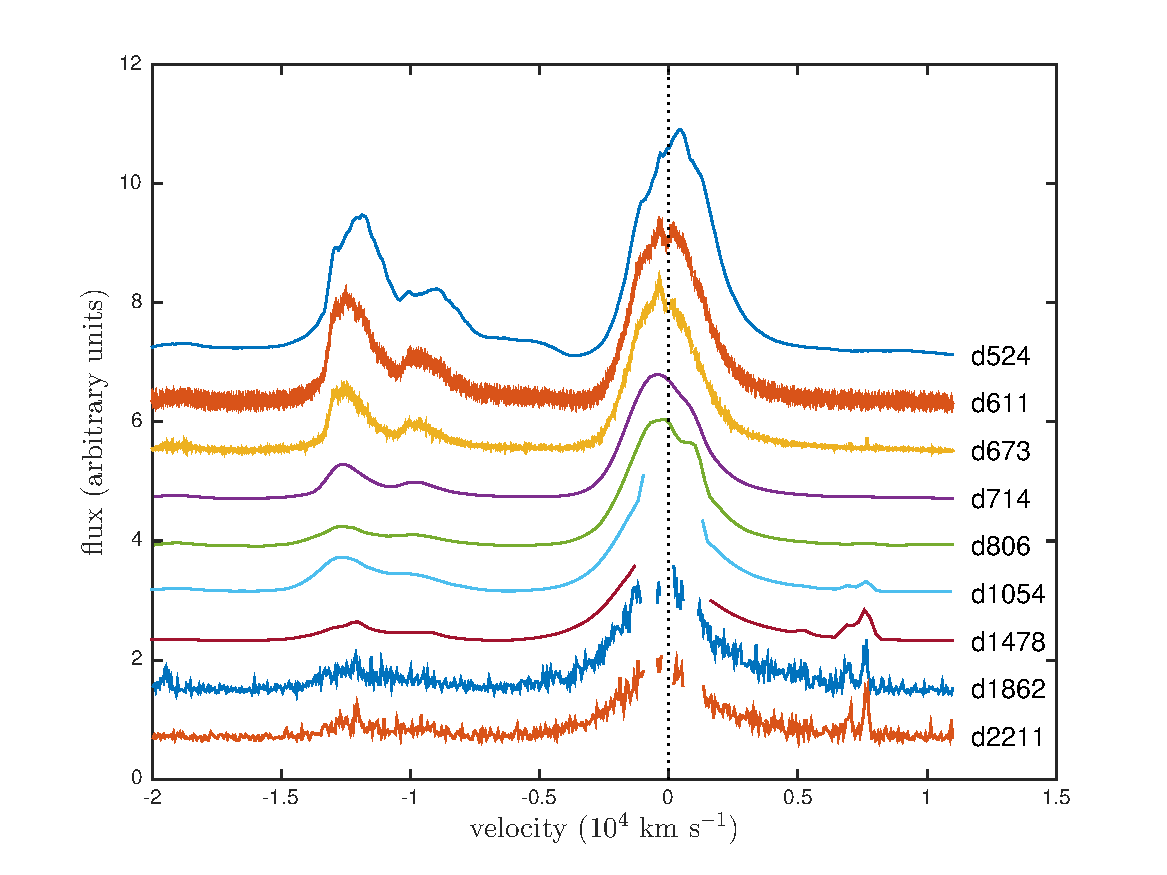
\includegraphics[trim =39 10 45 15,clip=true,scale=0.8]{chapters/chapter5/images/Ha_evol_early_1col2.pdf}
\caption{Archival data showing the evolution of the H$\alpha$ and
[O~{\sc i}] line profiles from SN~1987A at the earlier of the epochs considered. The 
spectral gaps at the last two epochs correspond to where narrow line 
emission from the equatorial ring has been removed. The spectra have been
continuum-subtracted and offsets have ben applied for display purposes.}
\label{Ha_evol_early}
%\end{center}
\end{figure}


Wavelength ranges encompassing the H$\alpha$ line and [O~{\sc 
i}]~$\lambda$6300,6363~\AA\ doublet were selected in order to trace their 
evolution from day 524, near the time of the first indications of dust 
formation \citep{Wooden1993}, to day 8020, near the current era. Optical 
spectroscopy obtained at the AAT using the Faint Object Red Spectrogaph 
(FORS) during the first two years after outburst was kindly supplied by Dr 
Raylee Stathakis \citep{Spyromilio1991, Spyromilio1993, Hanuschik1993} and 
optical spectra from the CTIO were donated by Dr Mark Phillips 
\citep{Suntzeff1991}.

The evolution of the H$\alpha$ and [O~{\sc i}] line profiles is presented 
in Figures \ref{Ha_evol_early} and \ref{Ha_evol_late}.  At later epochs, 
the broad H$\alpha$ profile emitted by the ejecta becomes contaminated by 
narrow line emission from the equatorial ring.  These lines have been 
removed for the purposes of modelling the broad line. A continuum fit has 
been subtracted from each spectrum and a velocity correction has been 
applied for a recession velocity of 287 km~s$^{-1}$ 
\citep{Groningsson2008}.


%FIGURE

\setlength{\tabcolsep}{5pt}
\begin{landscape}
\begin{table*}
	\begin{minipage}{180mm}
	\caption{Details of the archival data for SN 1987A.}
	\label{tb:data}
  	\begin{tabular}{@{} ccccccccl @{}}
    	\hline
	Date & Age & Telescope  & Inst & $\lambda_{min}$ & $\lambda_{max}$ & Res. & Res. & Reference \\
	& (days) & & &(\AA) & (\AA)& (\AA) & Power\\
	\hline
31 Jul 1988 & 524 & AAT & FORS & 5500 & 10190 & 20 & & \citet{Spyromilio1991} \\
26 Oct 1988 & 611 & AAT & UCLES & 6011 & 7336 &  & 30000 & \citet{Hanuschik1993, Spyromilio1993}\\
27 Dec 1988 & 673 & AAT & UCLES & 5702 & 10190 &  & 30000 & \citet{Hanuschik1993, Spyromilio1993}\\
06 Feb 1989 & 714 & CTIO-1.5m & Cass. & 6420 & 10380 & 16 & & \citet{Phillips1990}\\
09 May 1989 & 806 & CTIO-1.5m & Cass. & 6430 & 10330 & 16 & & \citet{Phillips1990}\\
12 Jan 1990 & 1054 & CTIO-4m & RC & 3565 & 10000 & 11 & & \cite{Suntzeff1991} \\
12 Mar 1991 & 1478 & CTIO-4m & RC & 3245 & 9175 & 11 & & \\
30 Mar 1992 & 1862 & HST & STIS & 4569 & 6818 & 4.4 &  & \citet{Wang1996}\\
14 Mar 1993 & 2211 & HST & STIS & 4569 & 6818 & 4.4 &  & \citet{Wang1996}\\
07 Jan 1995 & 2875 & HST & STIS & 4569 & 6818 & 4.4 &  & \citet{Chugai1997}\\
23 Sep 1996 & 3500 & HST & STIS & 4569 & 6818 & 4.4 &  \\ 
05 Jan 1997 & 3604 & HST & STIS & 4569 & 6818 & 4.4 &  \\
10 Dec 2000 & 5039 & VLT & UVES & 4760 & 6840 &  & 50000 & \citet{Groeningsson2006, Groeningsson2007}\\
06 Oct 2002 & 5704 & VLT & UVES & 4760 & 6840 &  & 50000 & \citet{Groeningsson2006, Groeningsson2007, Groningsson2008}\\
21 Mar 2005 & 6601 & VLT & UVES & 4760 & 6840 &  & 50000 &\citet{Groeningsson2006, Groeningsson2007}\\
23 Oct 2007 & 7547 & VLT & UVES & 4760 & 6840 &  & 50000 & \citet{Groeningsson2007}\\
07 Feb 2009 & 8020 & VLT & UVES & 4800 & 6800 &  & 50000 & \citet{Tziamtzis2010}\\
    \hline
  \end{tabular}
\end{minipage}
\end{table*}
\end{landscape}
\setlength{\tabcolsep}{12pt}

\subsection{Contamination of the H$\alpha$ profiles}

The H$\alpha$ profile at day 714 exhibits a very slight inflection visible 
at $V \approx +900$ km~s$^{-1}$.  By day 806, this slight inflection has 
developed into a noticeable shoulder in the line profile of H$\alpha$ (see 
Figure \ref{Ha}).

Although these features are similar in nature to features produced by dust 
absorption in the flat-topped region (as discussed in Section \ref{beta}), 
we conclude that this shoulder is an early appearance of the unresolved 
[NII] $\lambda$6583~\AA\ line from the equatorial ring \citep{Kozma1998b}.  Unresolved nebular [N~{\sc ii}] lines at $\lambda=$ 6583~\AA\ and 
$\lambda=$ 6548~\AA\ either side of the H$\alpha$ rest frame velocity at 
6563~\AA\ are certainly seen by day 1054 
%(see Figure \ref{d1054}) 
and have to be removed in order to consider the evolution of the broad 
H$\alpha$ profile (see Figure \ref{Ha_evol_early}). We do not remove this 
potential contaminant at earlier epochs but try to fit the broad line 
profiles around it.

\begin{figure}
\centering
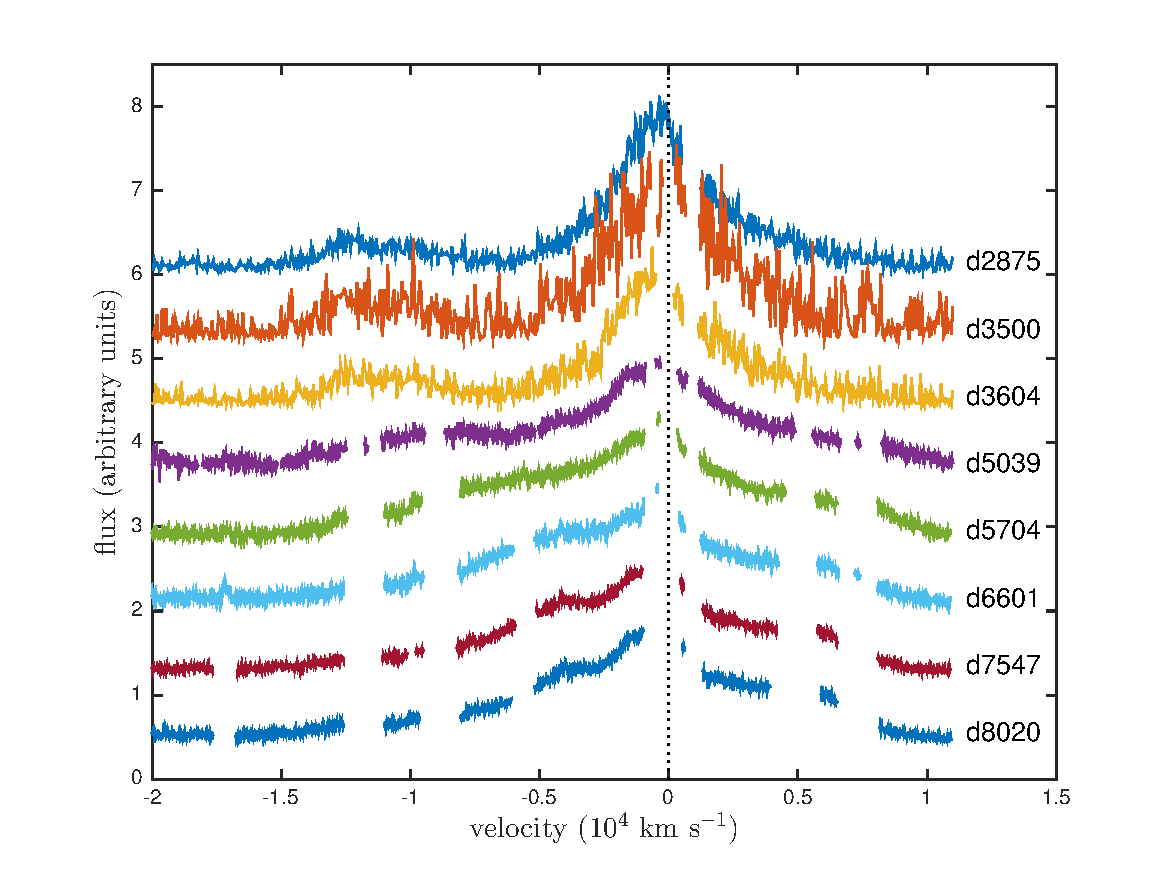
\includegraphics[trim =45 10 45 15,clip=true,scale=0.8]{chapters/chapter5/images/Ha_evol_late_1col.pdf}
\caption{Archival data showing the evolution of the H$\alpha$
line profile from SN~1987A at the later epochs. The spectral gaps 
correspond to where narrow line emission from the equatorial ring has been 
removed. The spectra have been continuum-subtracted and offsets applied 
for display purposes.}
\label{Ha_evol_late}
%\end{center}
\end{figure}

\begin{table}
\centering
\caption{H$\alpha$ full-width half-maxima (FWHM) and the half-width zero 
intensities (HWZI) determined by the zero intensity velocity on the 
blue side of the line.  The tabulated line widths have been corrected for the relevant instrumental resolution.}
\begin{tabular}{c cc}
day & FWHM (\AA) & HWZI (\AA) \\
\hline
524 & 3200 & 3600 \\
611 & 2700 & 3400 \\
673 & 1600 & 3700 \\
714 & 3100 & 4500 \\
806 & 3200 & 5500 \\
1054 & 2100 & 5600 \\
1478 & 1400 & 6600 \\
1862 & 1600 & 6800 \\
2211 & 1400 & 6700 \\
2875 & 2700 & 6700 \\
3500 & 3500 & 7000 \\
3604 & 2100 & 7000

\end{tabular}

\label{FWHM}
\end{table}%


 
By day 1054, all three of the narrow nebular lines are strong.  They 
remain unresolved in the low spectral resolution CTIO data at days 1054 
and 1478 and therefore contaminate the entire central region of the 
H$\alpha$ line profile.  Their presence renders two CTIO H$\alpha$ 
profiles from days 1054 and 1478 unusable for modelling purposes.  The HST 
and VLT H$\alpha$ profiles at later epochs ($\ge$ 1862 days) have a higher 
spectral resolution and it was therefore easier to remove the narrower 
[N~{\sc ii}] and H$\alpha$ lines from the broad H$\alpha$ profiles (for 
example Figures \ref{Ha_evol_early} and \ref{Ha_evol_late}). Although this 
does remove a potentially informative section of the profile ($+500$ 
km~s$^{-1}<v<+1500$ km~s$^{-1}$), we achieve good fits to the overall line 
profiles at these epochs.


\subsection{The evolution of the maximum and minimum velocities}

For a freely expanding medium, the velocity of any fractional radial 
element should not change with time.  The maximum velocity of any 
line-emitting region is therefore expected to be constant.  However, at 
the epochs we consider here, it appears that the maximum velocities of the 
H$\alpha$ line, as determined by the velocity at zero intensity on the 
blue side, generally increase over time (see Table \ref{FWHM}).  We 
attribute this to the start of the freeze-out phase in the outer regions 
of the ejecta, while the hydrogen neutral fraction is still increasing in 
the denser inner regions \citep{Danziger1991,Fransson1993}.

The onset of a fixed ionization structure in the ejecta causes the rate of 
H$\alpha$ flux decline to slow.  Since the outer, faster moving regions 
reach this state at earlier times than the inner, slower moving regions, 
the relative flux contribution of the outer regions is increased.  At 
early epochs ($t<900$ days) the flux contribution from hydrogen in the 
core dominates the overall H$\alpha$ flux, whereas at later epochs ($t > 
900$ days) the flux from the envelope dominates \citep{Fransson1993, 
Kozma1998a}.  This shift likely explains apparent broadening of the line 
with the higher velocity material becoming increasingly noticeable in the 
line profiles.  This may also explain the increase in HWZI velocities at 
these epochs with the relative flux from the very densest regions dropping 
more rapidly relative to the outer line-emitting region. The full-width 
half maximum (FWHM) remains relatively steady (see Table 
\ref{FWHM}). However, the FWHM values presented in Table \ref{FWHM} were difficult 
to determine accurately since the peak of the broad line profile is 
contaminated by narrow line emission from the equatorial ring.

%%%%%%%%%%%%%%%%%%%%   SPECTRA   %%%%%%%%%%%%%%%%%%%%%%%%%%%

\section{Modelling SN~1987A}
\label{results}
\begin{figure}
\centering
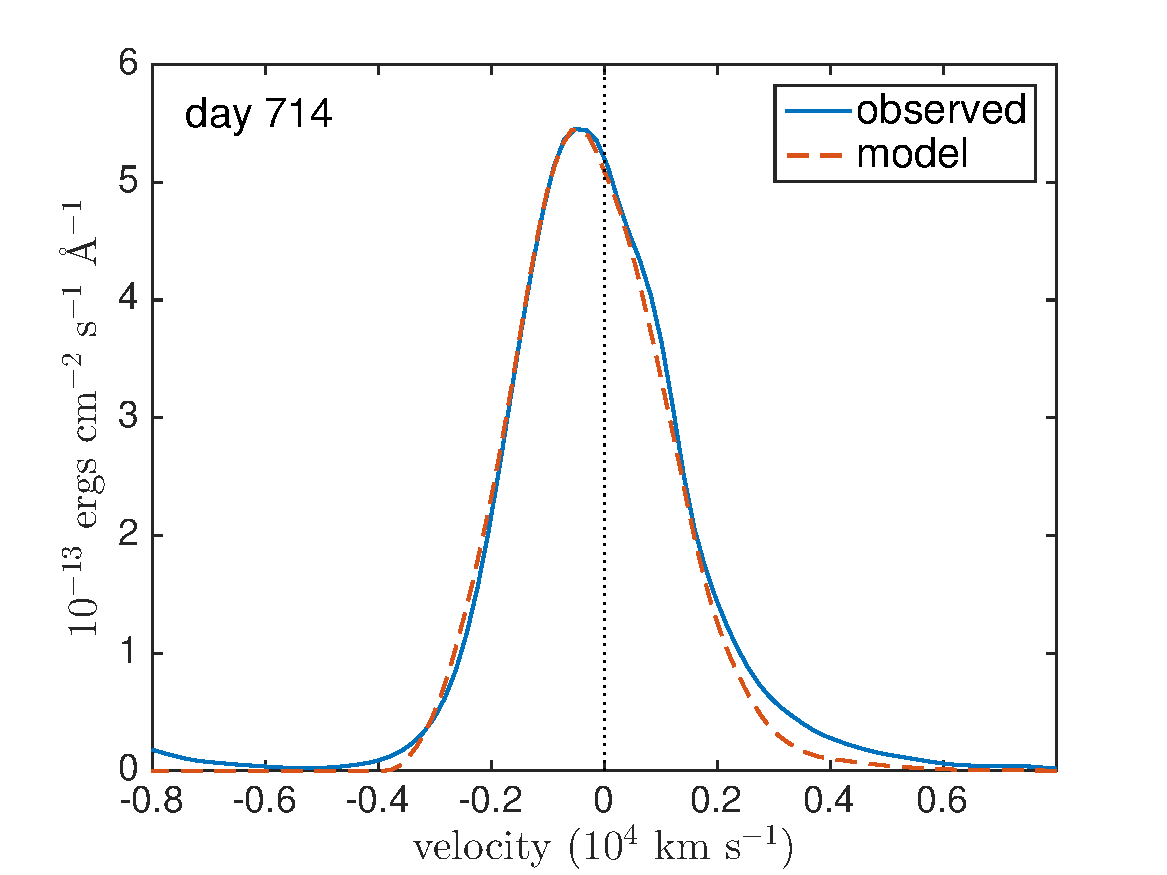
\includegraphics[trim =33 10 45 15,clip=true,scale=0.7]{chapters/chapter5/images/smooth/d714Ha_smooth_amC_MRN.pdf}
\caption{Amorphous carbon smooth dust fit to the day 714 H$\alpha$ 
line of SN~1987A using an MRN size distribution,
illustrating the underestimation of the red scattering wing for small 
grain radii.  Model parameters are the same as the smooth dust fit for 
day 714 (Table \ref{smooth1}) except for the 
grain size distribution and dust mass:  $M_{dust}=8.0 \times 10^{-6} 
M_{\odot}$, $a_{min}=0.005~\mu$m, $a_{max}=0.25~\mu$m and $n(a) \propto 
a^{-3.5}$.}
\label{MRN}

\end{figure}

\begin{figure*}
\centering
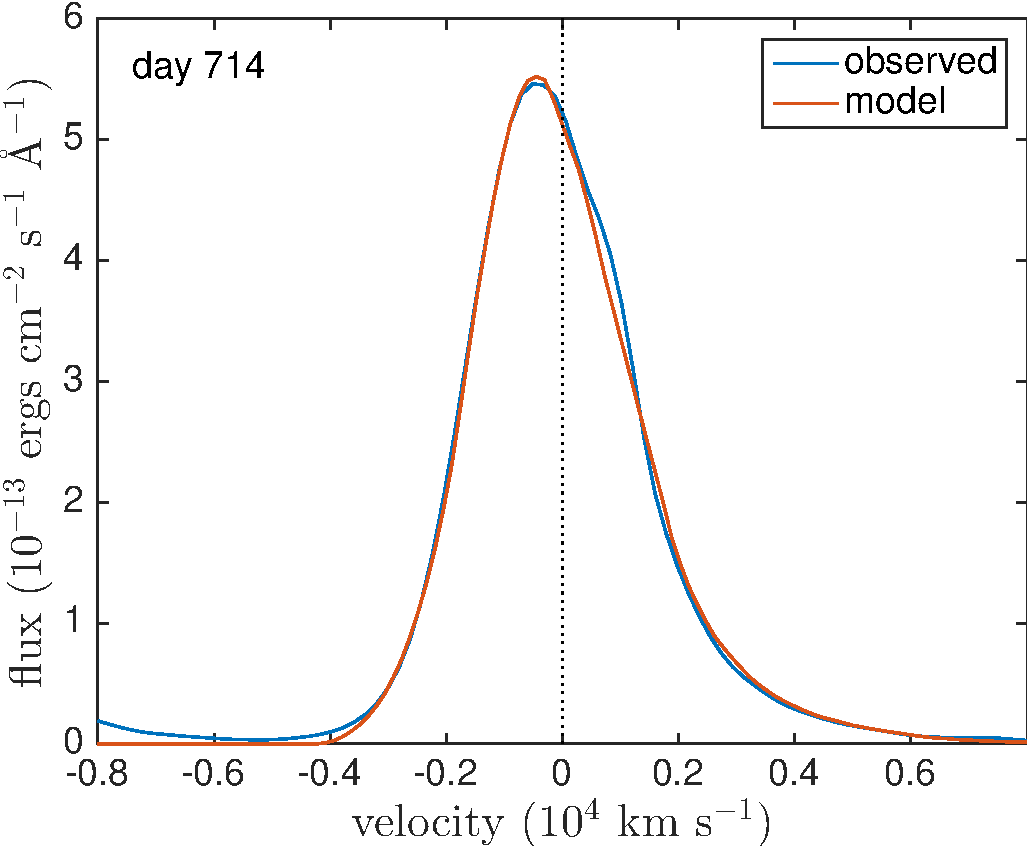
\includegraphics[trim =0 0 0 0,clip=true,scale=0.4]{chapters/chapter5/images/smooth/best_fit/d714Ha_new.pdf}
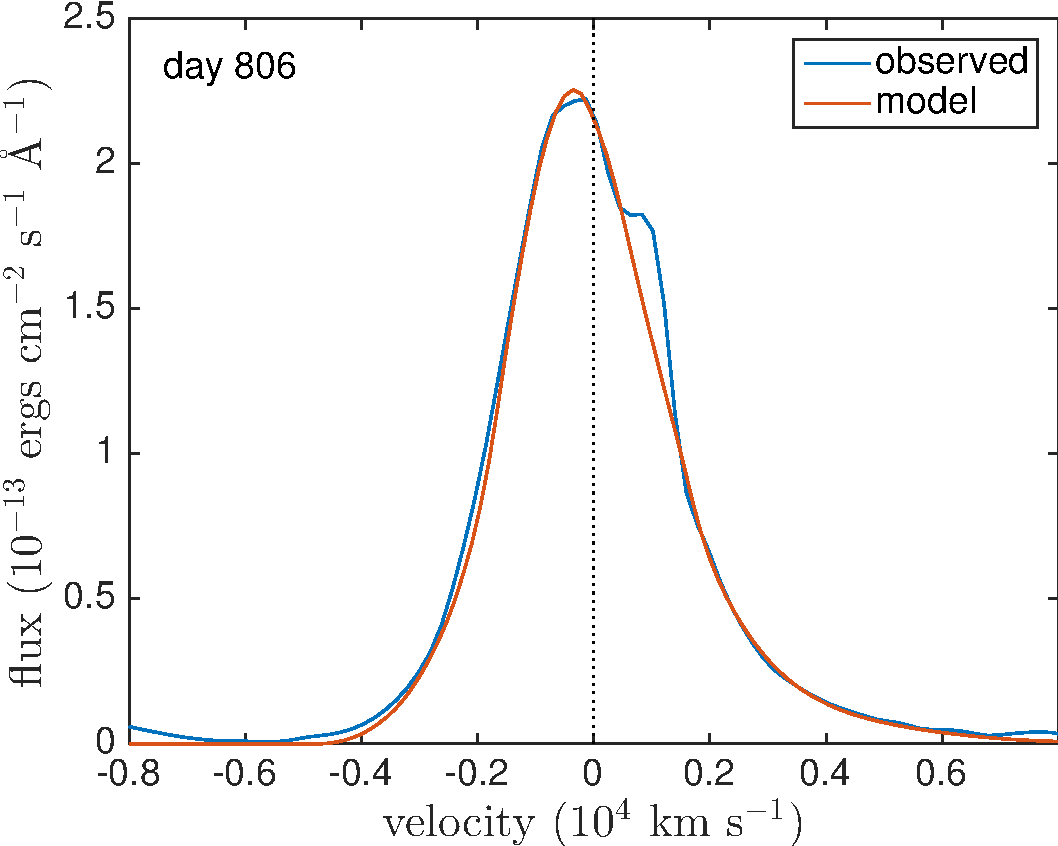
\includegraphics[trim =25 0 0 0,clip=true,scale=0.4]{chapters/chapter5/images/smooth/best_fit/d806Ha_new.pdf}

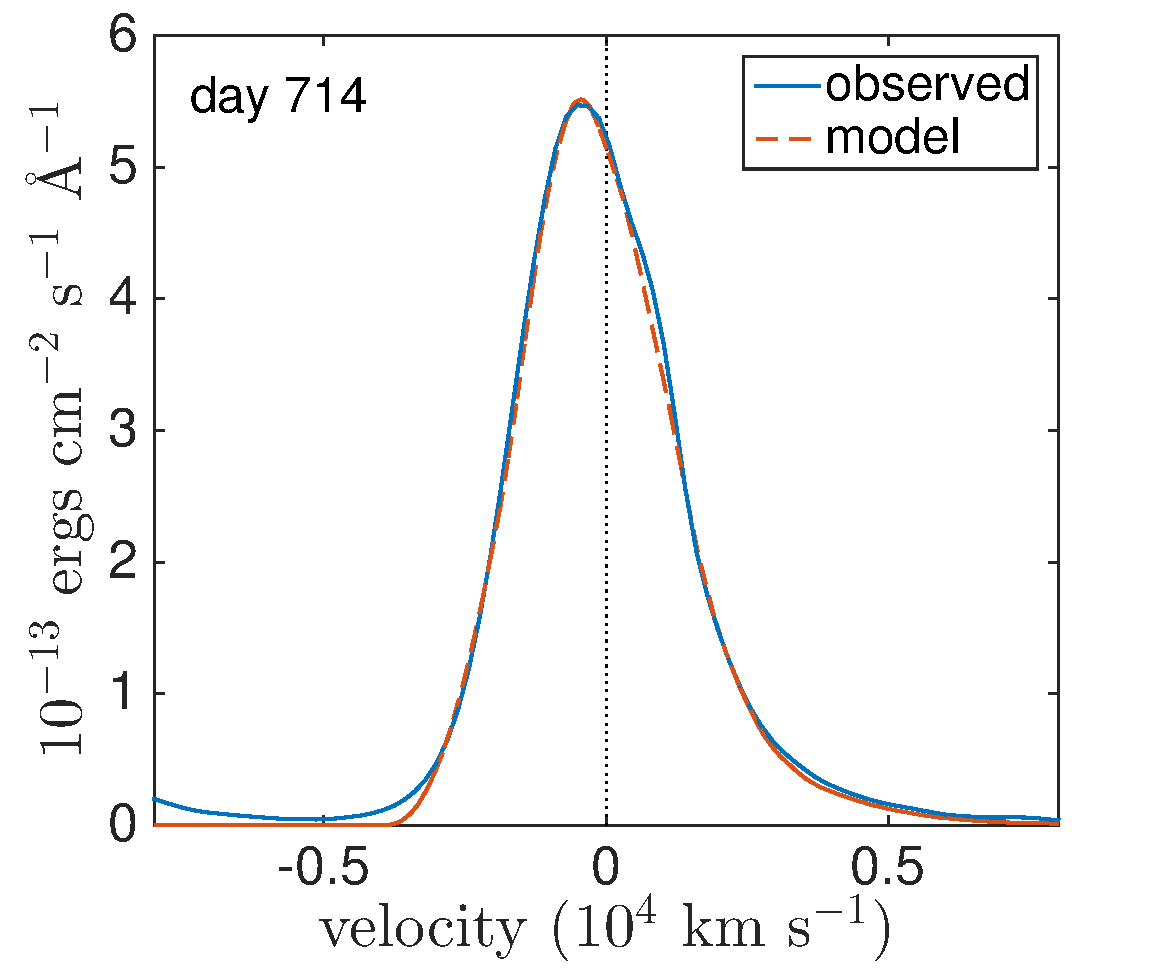
\includegraphics[trim =25 0 0 0,clip=true,scale=0.4]{chapters/chapter5/images/clump_1/best_fit/d714Ha_new.pdf}
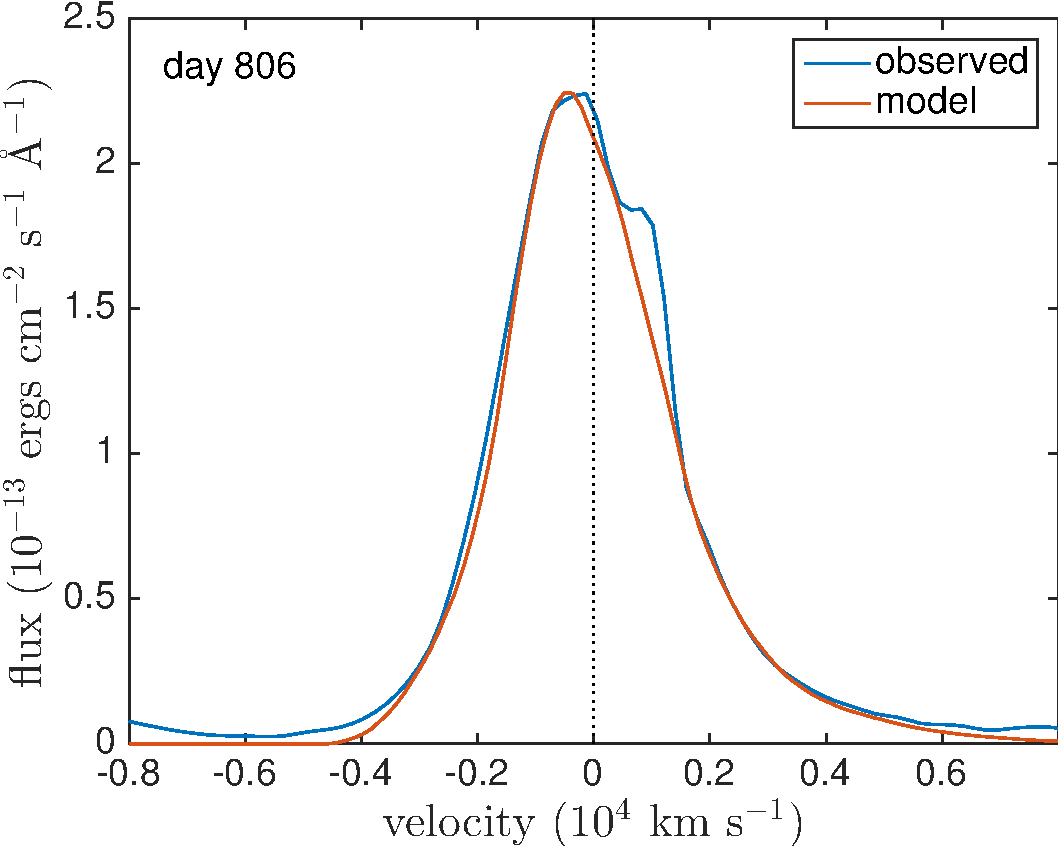
\includegraphics[trim =25 0 0 0,clip=true,scale=0.4]{chapters/chapter5/images/clump_1/best_fit/d806Ha_new.pdf}
\caption{Best model fits to the SN~1987A H$\alpha$ line at day 714 
and day 806 for the parameters detailed in Tables \ref{smooth1} and \ref{clumped1}. The two fits on the top are smooth dust models using amorphous carbon grains of radius $a=0.35~\mu$m and the two fits on the bottom are clumped dust models using amophous carbon grains of radius $a=0.6~\mu$m.}
\label{Ha}

\end{figure*}


We have modelled the H$\alpha$ line of SN~1987A at days 714, 806, 1862, 
2211, 2875, 3500 and 3604, and the [O~{\sc i}]~$\lambda$6300,6363~\AA\ 
doublet at days 714, 806, 1054 and 1478.  After day 3604 the H$\alpha$ 
profile begins to become dominated by emission from the reverse shock and 
the structure of the emitting region may no longer be approximated by a 
single shell model as we do here \citep{Fransson2013}.  The [O~{\sc 
i}]~$\lambda$6300,6363~\AA\ doublet becomes too weak to model after day 
1478 (see Figure \ref{Ha_evol_early}).  We continue to adopt a velocity 
profile $V(r) = \frac{V_{max}}{R_{max}}r$ and treat the variable 
parameters listed at the start of Section \ref{ps}.  Whilst the albedo and 
optical depth are not varied directly, they are altered by adjusting the 
dust mass, $M_{dust}$, and the grain size, $a$, which together determine 
the albedo and optical depth via Mie theory and the optical properties of 
the dust.

\setlength{\tabcolsep}{10pt}
\begin{table}
\caption{Observed luminosities of the H$\alpha$ line and estimated 
electron scattering optical depths from $R_{in}$ to $R_{out}$ for the 
radii detailed in Tables \ref{smooth1} to \ref{clumped1} based on an 
assumed gas temperature of 10,000~K.}
\centering
\begin{tabular}{@{}cccccc@{}}
\hline
& \multicolumn{2}{c}{H$\alpha$} &  \multicolumn{2}{c}{[O~{\sc i}]}  \\
day &  $L_{obs}$ & $L_{undep}$/  &  $L_{obs}$ & $L_{undep}$/   & $\tau_e$ \\
& (10$^{37}$ erg s$^{-1}$) &$L_{obs}$& (10$^{37}$ erg s$^{-1}$) & $L_{obs}$& ($10^{-2}$) \\
\hline
714 & 1.36 & 1.65 &0.313&3.57& 1.44  \\
806 & 0.57 & 1.77 &0.0942&3.57& 0.840 \\
1054 &&&0.0242 & 3.23\\
1478 &&& 0.00185&2.70 \\
1862 & 0.0063 & 2.06 &&& 0.159  \\
2211 & 0.0041 & 2.07 &&& 0.0378  \\
2875 & 0.0019 & 2.84 & & &0.0219  \\
3500 & 0.00079 & 3.16 & &&0.0125  \\
3604 & 0.00098 & 3.27 &&&0.0149  \\

\hline
\end{tabular}

\label{tau_e}
\end{table}%
\setlength{\tabcolsep}{8pt}


In all models, the ejecta occupies a shell with inner radius $R_{in}$ and 
outer radius $R_{out}$.  Packets are emitted according to a smooth density 
profile assuming recombination or collisional excitation such that $i(r) 
\propto \rho(r)^2 \propto r^{-2\beta}$.  Initially the dust is considered 
to have a smooth density distribution and is assumed to be coupled to the 
gas so as to follow the same radial profile.  A clumped distribution of 
dust is considered later (see Section \ref{clumped_models}).

We estimate the electron scattering optical depths assuming an electron 
temperature of 10,000~K between $R_{in}$ and $R_{out}$ based on the 
observed fluxes of the H$\alpha$ line.  A temperature of 10,000~K is 
likely too high at the epochs considered but we adopt it in order
not to underestimate electron scattering optical depths.  The values 
we calculate from the observed H$\alpha$ luminosities are listed in Table 
\ref{tau_e}.  Since the electron scattering optical depths at these epochs 
are negligibly small we therefore do not include electron scattering in 
the models.




There is rarely a unique set of parameters that provide the best fit to 
the data.  However, the majority of the parameters of interest can be well 
constrained from our modelling by considering different elements of the 
shape of the profile.  In particular, by constructing fits to the data 
using minimum and maximum limits for the grain radius, credible lower and 
upper bounds on the dust mass formed within the ejecta may be derived.  
We present here fits to the data obtained using both small and large 
values of the grain radius $a$ since it is the grain size which has the 
most significant effect on the overall dust mass required to reproduce the 
line profile (see Section \ref{params}).


All of our models are of a dusty medium composed solely of amorphous 
carbon grains. We use the optical constants from the BE sample presented 
by \citet{Zubko1996}.  Although previous SED modelling of SN~1987A  
limited the fraction of silicates present in the dusty ejecta to a maximum 
of 15\% (\citet{Ercolano2007}, W15), the recent work of \citet{Dwek2015} has suggested that a large mass of mostly silicate dust may have formed at early epochs ($\sim$ 615 days).  It is therefore useful to consider the effects 
on our models of using silicate dust.  We discuss this in detail in 
Sections \ref{species} and \ref{dwek}.

For each profile, the maximum velocity is initially identified from the 
data as the point where the emission vanishes on the blue side and is then 
varied throughout the modelling in order to produce the best fit.  The 
equivalent point on the red side is indeterminate from observations due to 
the effects of dust scattering.  We determine the approximate value of 
$V_{min}$ by examining the width of the profile near its peak. On the red side the theoretical minimum velocity often 
falls at a similar velocity to the 6583\AA\ line so any dust-induced 
features near this wavelength that would allow a more accurate 
determination of $V_{min}$ can be overwhelmed by the nebular line.  
Having determined the minimum and maximum velocities, the ratio of the 
inner and outer radii of the supernova ejecta can be determined since 
$R_{in}/R_{out}=V_{min}/V_{max}$.  The outer radius is calculated from the 
epoch and the maximum velocity.

The only parameters that  remain to be determined are the exponent of 
the density profile $\beta$, the mean grain radius and the total dust 
mass.  The shape of the blue wing is solely a product of the density 
profile and the dust mass; the height and shape of the red wing is a 
product of these and also of the scattering efficiency of the grains (the 
albedo $\omega$); the extent and shape of the asymmetry in the flat-topped 
portion of the profile is a function of only the total dust optical depth 
determined by the dust mass and the grain radius.  By iterating over these 
three parameters, an excellent fit to the data can usually be 
obtained.

Models are produced in the same manner for the [O~{\sc 
i}]~$\lambda$6300,6363~\AA\ doublet as for the single H$\alpha$ line, with 
each component of the doublet being modelled independently and the 
resulting profiles added according to a specified ratio.  Although the 
theoretical intrinsic flux ratio is 3.1 for optically thin emission \citep{Storey2000}, the 
actual ratio between the two components can be affected by self-absorption 
\citep{Li1992} and we therefore left it as a free parameter.  The deduced 
doublet ratios are listed in Tables \ref{smooth1}, \ref{clumped1} and 
\ref{clumped2}.


\begin{figure*}
\centering
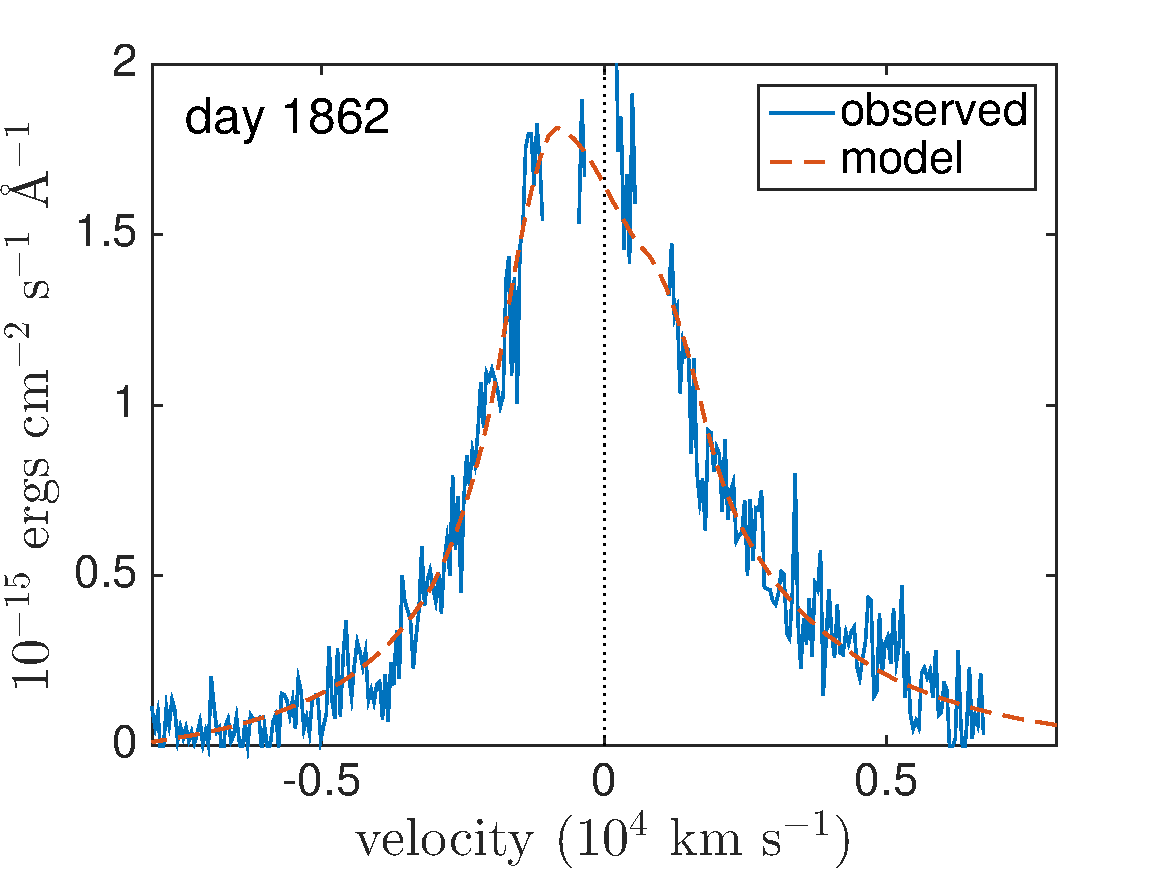
\includegraphics[trim =0 0 0 0,clip=true,scale=0.4]{chapters/chapter5/images/smooth/best_fit/d1862Ha.pdf}
\hspace{2mm}
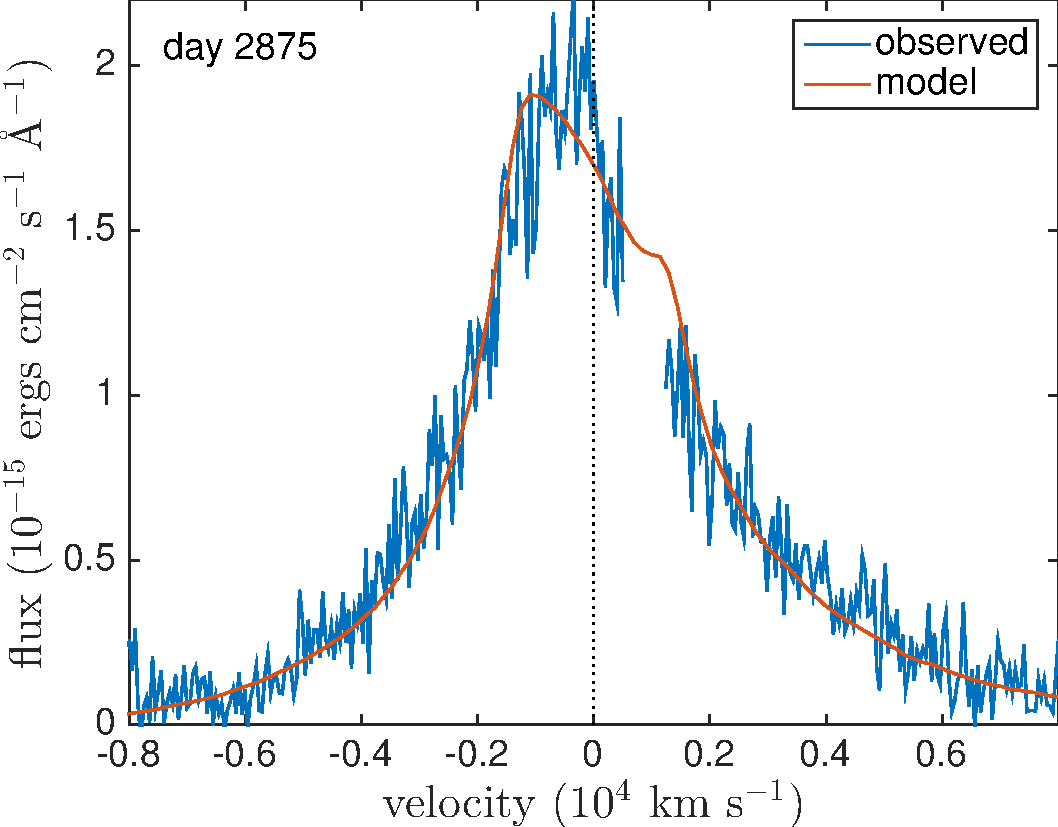
\includegraphics[trim =25 0 0 0,clip=true,scale=0.4]{chapters/chapter5/images/smooth/best_fit/d2875Ha.pdf}

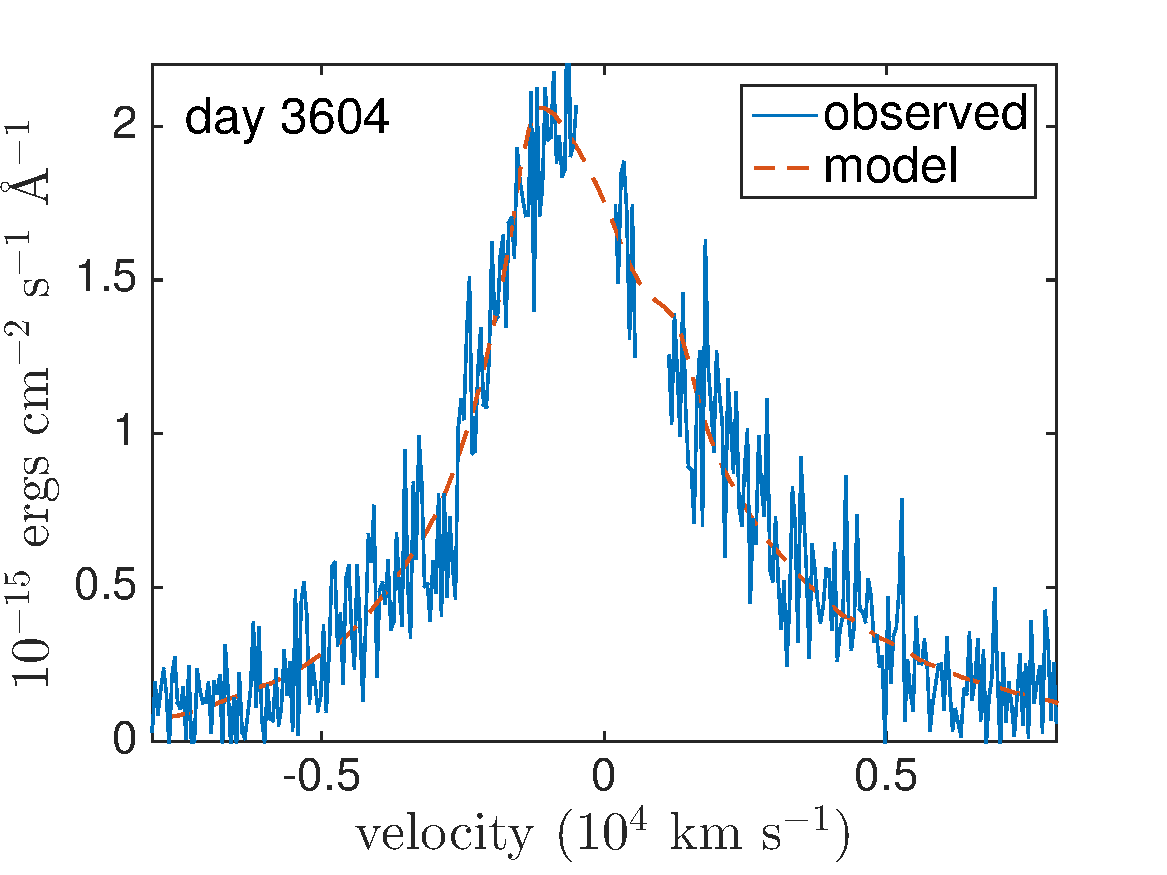
\includegraphics[trim =0 0 0 -30,clip=true,scale=0.4]{chapters/chapter5/images/smooth/best_fit/d3604Ha.pdf}
\caption{Best model fits to the SN~1987A H$\alpha$ line at days 1862, 2875 and 
3604 for the parameters detailed in Tables \ref{smooth1}, \ref{clumped1} and \ref{clumped2}.  On the top row are smooth model fits with amorphous carbon grains of radius $a=0.35~\mu$m.  On the middle and bottom rows are clumped model fits with amorphous carbon grains of radii $a=0.6~\mu$m and $a=3.5~\mu$m respectively.}
\label{}
\end{figure*}

\begin{figure*}
\centering
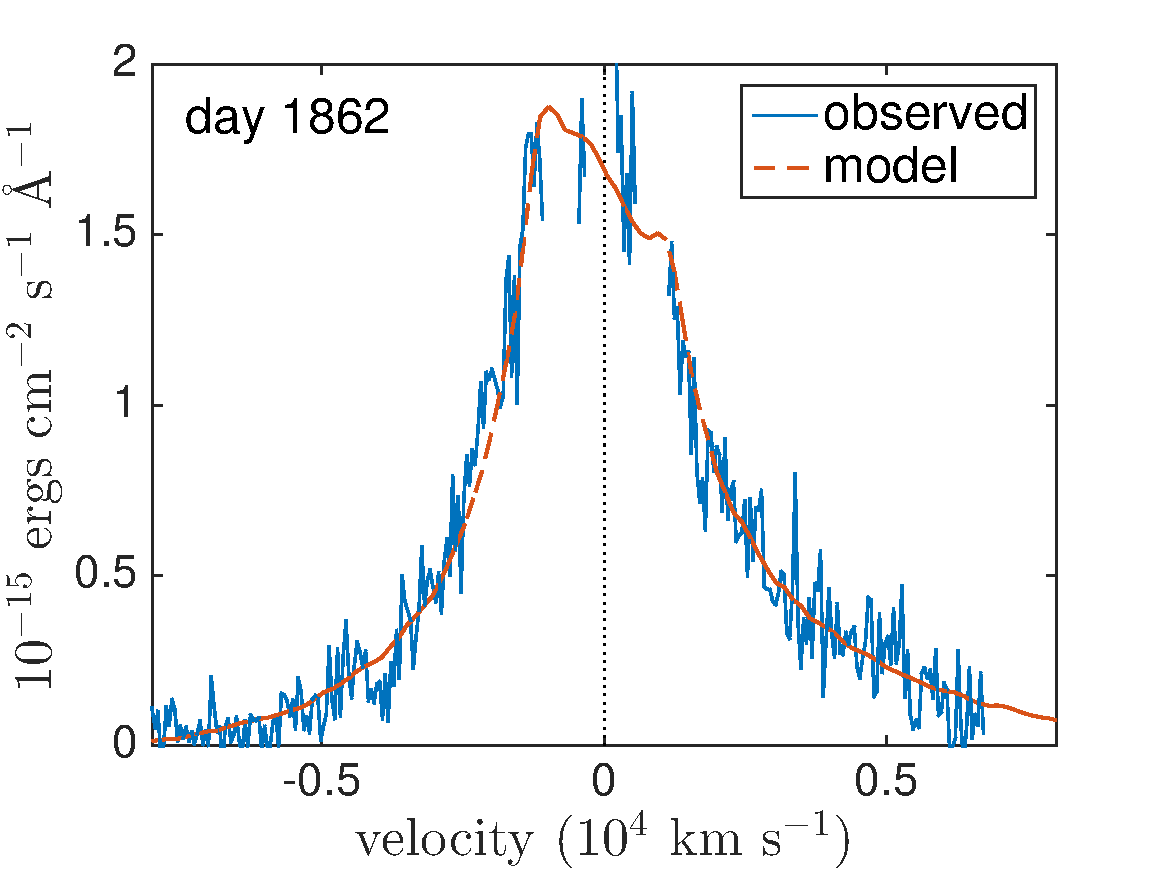
\includegraphics[trim =0 25 0 -20,clip=true,scale=0.4]{chapters/chapter5/images/clump_1/best_fit/d1862Ha.pdf}
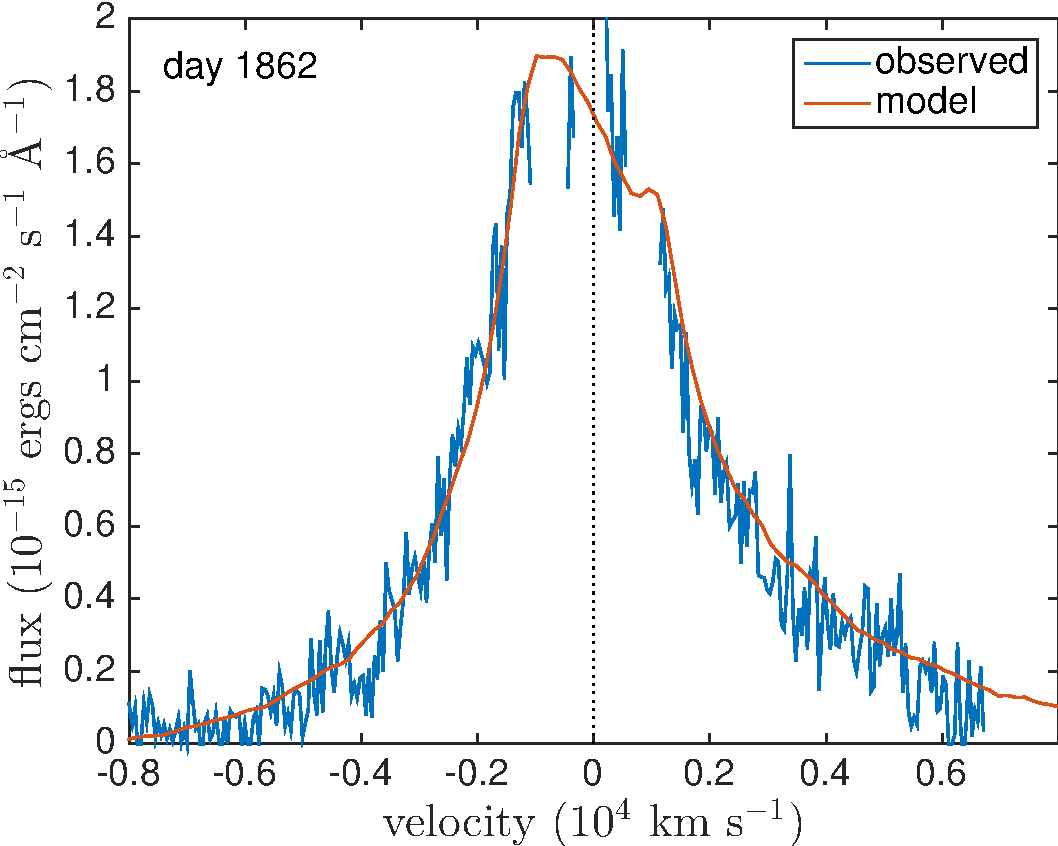
\includegraphics[trim =25 25 0 -20,clip=true,scale=0.4]{chapters/chapter5/images/clump_1/maximum/d1862Ha.pdf}

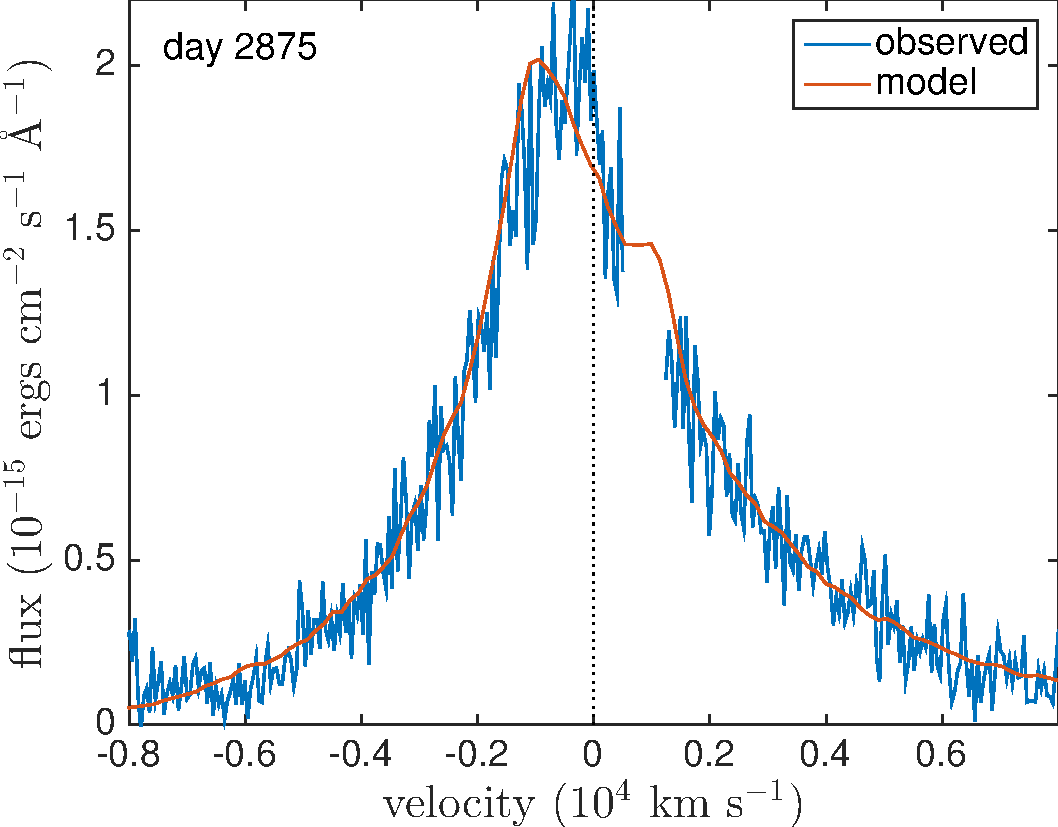
\includegraphics[trim =0 25 0 -20 ,clip=true,scale=0.4]{chapters/chapter5/images/clump_1/best_fit/d2875Ha.pdf}
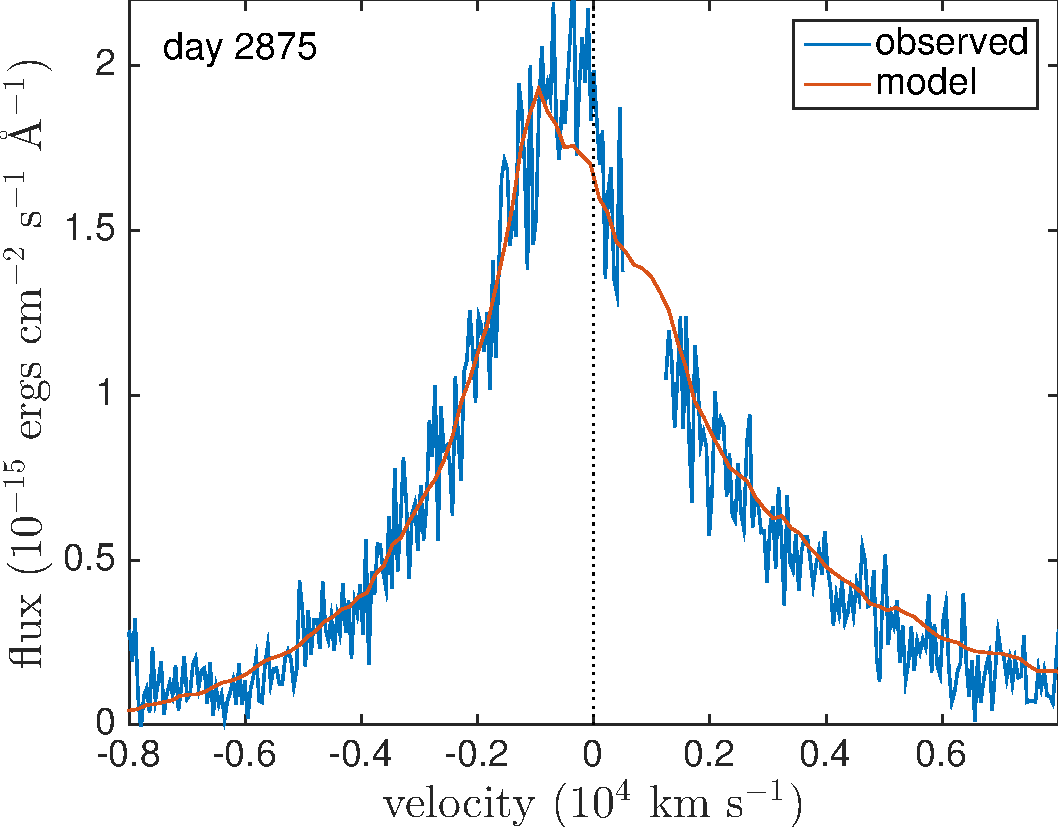
\includegraphics[trim =25 25 0 -20,clip=true,scale=0.4]{chapters/chapter5/images/clump_1/maximum/d2875Ha.pdf}

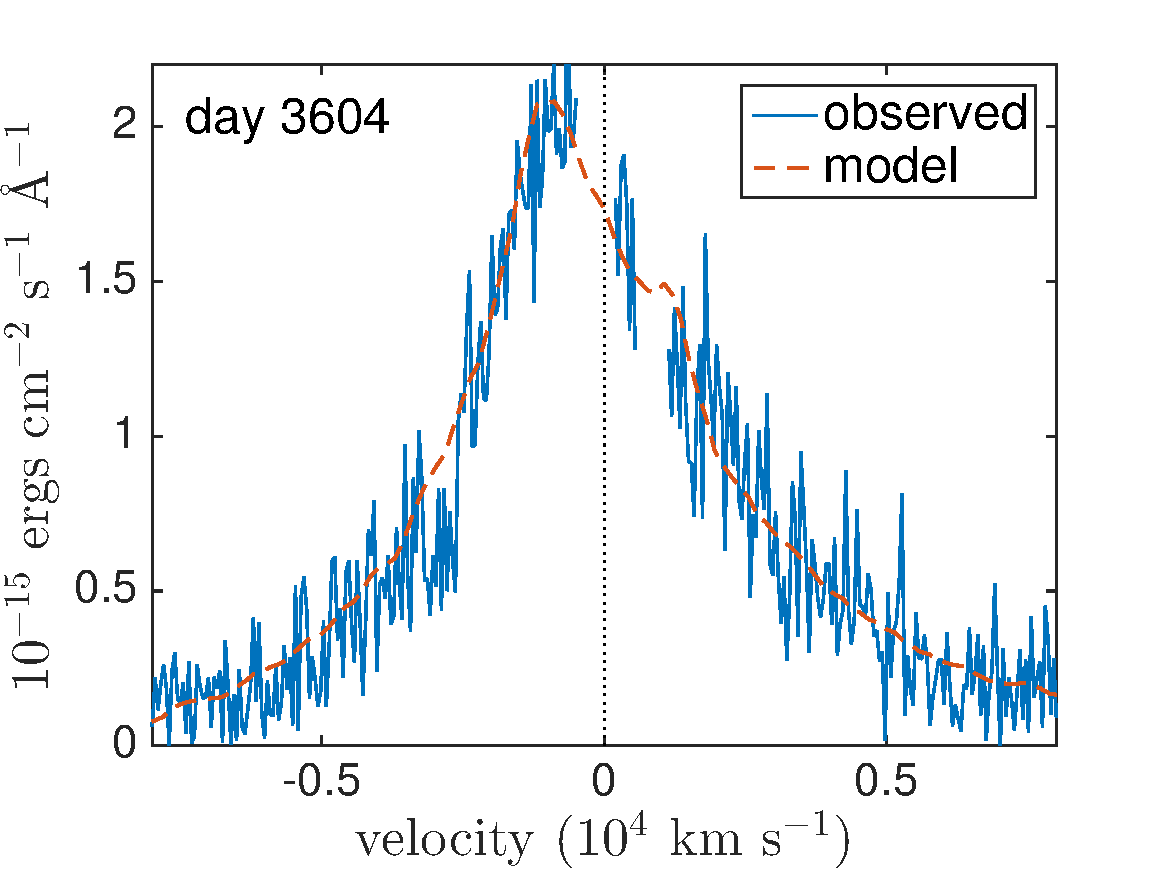
\includegraphics[trim =0 0 0 -20,clip=true,scale=0.4]{chapters/chapter5/images/clump_1/best_fit/d3604Ha.pdf}
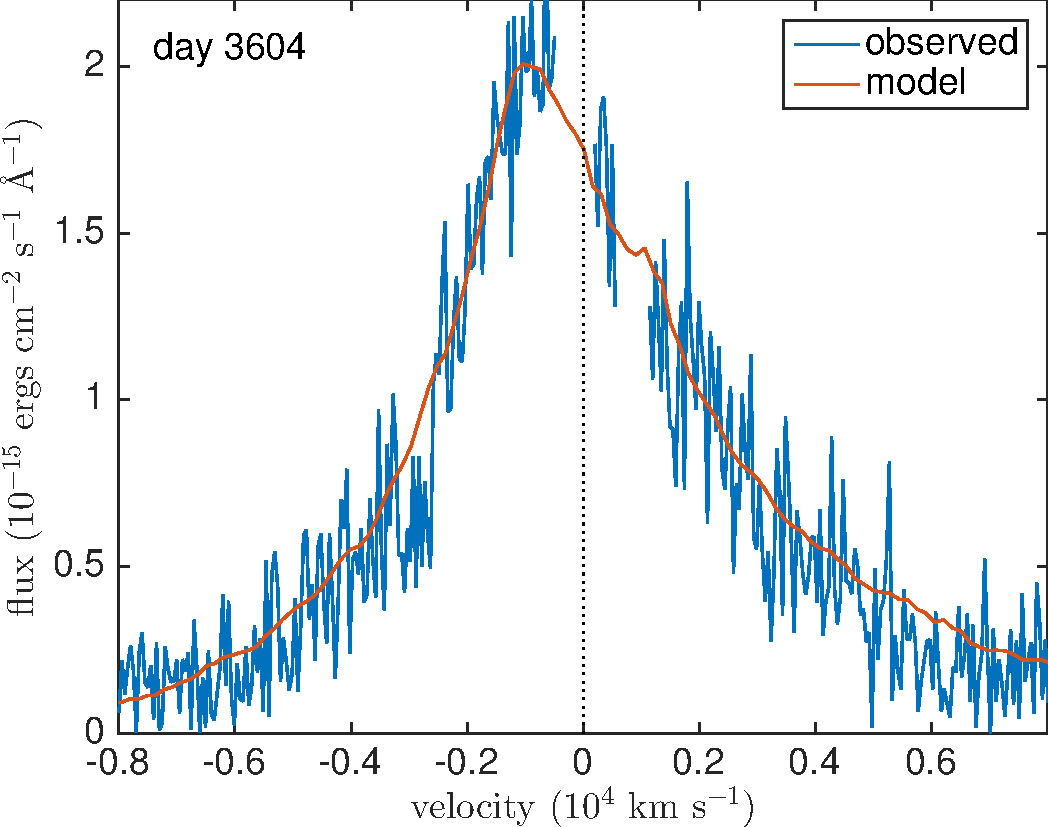
\includegraphics[trim =25 0 0 -20,clip=true,scale=0.4]{chapters/chapter5/images/clump_1/maximum/d3604Ha.pdf}
\vspace{8mm}
\caption{Best model fits to the SN~1987A H$\alpha$ line at days 1862, 2875 and 
3604 for the parameters detailed in Tables \ref{smooth1}, \ref{clumped1} and \ref{clumped2}.  On the top row are smooth model fits with amorphous carbon grains of radius $a=0.35~\mu$m.  On the middle and bottom rows are clumped model fits with amorphous carbon grains of radii $a=0.6~\mu$m and $a=3.5~\mu$m respectively.}
\label{d1862_3604}

\end{figure*}

For all lines, though particularly at very late epochs, even small 
fluctuations in the adopted value of the continuum level can have a 
substantial effect on the fit to the resulting profile.  Since it is not 
feasible to establish the level of the continuum so precisely, the value 
of the continuum has been left as a free parameter that may be adjusted 
(to within sensible margins) in order to allow for the widest possible 
dust mass range to be determined.  We generally find it is necessary to 
assume a continuum level that is slightly lower where the dust mass is 
higher.  The [O~{\sc i}]$\lambda$6300,6363~\AA\ doublets at days 1054 and 
1478 are weak relative to the continuum and are also blended with the 
wings of other lines making it difficult to fit their wings accurately.  
We aim to fit the lines between approximately -3000 km s$^{-1}$ and +5000 
km s$^{-1}$ but present a wider velocity range for context (for example 
see Figure \ref{OI_smooth}).


Fits to the H$\alpha$ line profile at days 2211 and 3500 are omitted for 
the sake of space but are very similar to those of days 1862 to 3604.  
All profiles have been smoothed to approximately the same resolution as 
the observed profiles using a moving-average procedure.  Parameters for 
the models at all epochs including days 2211 and 3500 are detailed in 
Tables \ref{smooth1} to \ref{clumped2}.


\subsection{Smooth Density Models for SN 1987A}
\label{smooth_models}

Even at the earliest epochs there is a substantial wing on the red side of 
the H$\alpha$ line profile that cannot be fitted by scattering from moving 
grains with a low albedo.  The minimum required albedo is approximately 
$\omega \approx 0.5$ implying relatively large grain radii.  As previously 
discussed, the larger the grain size the larger the mass of dust required 
to reproduce the same optical depth.  Figure \ref{MRN} illustrates the fit 
for the day 714 H$\alpha$ profile for the case where a classic MRN 
\citep{Mathis1977} grain size distribution is adopted, with $a_{min}=0.005 
\mu$m, $a_{max}=0.25~\mu$m and $n(a) \propto a^{-3.5}$.  It can be seen 
clearly that the extended red wing is significantly underestimated.  
Since the albedo of amorphous carbon grains varies significantly with 
grain radius (see Figure \ref{albedo_grain}) we can establish a strong 
lower bound to the mean dust grain radius, which we estimate to be $a \ge 
0.35~\mu$m.  This is the smallest grain size that is still capable of 
reproducing the red scattering wing at all epochs and we therefore use 
this lower limit value throughout our smooth density modelling.


The inner and outer radii of the ejecta are calculated at each epoch from 
the maximum velocity used, the day number and the specified ratio 
$R_{in}/R_{out}$.  The radii generated are consistent with those used in 
previous models of SN 1987A (\citet{Ercolano2007}, W15) and the 
minimum velocities for both the [O~{\sc i}] and H$\alpha$ line emitting 
regions are relatively consistent with those obtained by \citet{Kozma1998b} 
who estimate that  hydrogen extends into the core to a depth of 
$\lesssim 700$~km~s$^{-1}$ and the oxygen reaches down to $\sim 
400$~km~s$^{-1}$.  They are also consistent with predictions from 3D 
explosion models at the time of shock-breakout that predict the oxygen to 
reach to a depth of $\sim 200$~km~s$^{-1}$ 
\citep{Hammer2010,Wongwathanarat2015}. Figures \ref{Ha} and 
\ref{d1862_3604} show the best fits to the data for days 714 to 3604 
whilst Table \ref{smooth1} details the parameters used.

It can be seen from Tables \ref{smooth1} to \ref{clumped2} that, in order 
to reproduce the blueshifts seen in the [O~{\sc 
i}]~$\lambda$6300,6363~\AA\ doublet, considerably larger dust masses are 
required than to fit the H$\alpha$ line at the same epoch.  Although the 
same maximum velocities and therefore outer radii are used in our [O~{\sc 
i}] and H$\alpha$ models, the inner radii for the [O~{\sc i}] models are 
significantly smaller and the density distribution much steeper.  This 
implies that [O~{\sc i}] is concentrated towards the centre of the 
ejecta whereas H$\alpha$ is more diffuse.  This is broadly in 
agreement with 3D explosion dynamics models that suggest that a few hours 
after the explosion the heavier elements will, in comparison to hydrogen, 
be located more centrally in the ejecta with ``bullets" of heavier 
material reaching the outer edges \citep{Hammer2010}.  If dust is forming 
in the inner regions of the ejecta then the majority of the [O~{\sc i}] 
emission must travel through the newly formed dust whereas the more 
diffuse H$\alpha$ emission has a greater chance of escaping unaffected.  
This may explain the difference between the dust masses needed for the 
[O~{\sc i}] and H$\alpha$ models.


\begin{landscape}

\begin{table*}
\centering
	\begin{minipage}{180mm}
	\caption{The parameters used for the best fitting 
smooth models of SN~1987A with amorphous carbon grains of radius $a=0.35~\mu$m.  Optical depths are given from $R_{in}$ to $R_{out}$ at $\lambda = 6563$~\AA\ for H$\alpha$ and $\lambda = 6300$~\AA\ for [O~{\sc i}]. Values of $\tau_V$ are very close to the quoted values of $\tau_{H\alpha}$.}
	\label{smooth1}
	\centering
  	\begin{tabular}{@{} cccccccccccc @{}}
    	\hline
 & day & $V_{max}$ & $V_{min}$ & $R_{in}/R_{out}$ & $\beta$ & $M_{dust}$ & $R_{out}$ & $R_{in}$ & [O~{\sc i}] ratio & $\tau_{\lambda}$   \\
	&& (km~s$^{-1} $)& (km~s$^{-1} $) & & & ($M_{\odot}$) & (cm) & (cm) \\
	\hline


[O~{\sc i}]  & 714 & 3250 & 228 & 0.07  & 2.9 & 9.65$\times 10^{-5}$ & 2.00$\times 10^{16}$ & 1.40$\times 10^{15}$ & 2.6 & 3.60  \\ \relax
[O~{\sc i}]  & 806 & 4000 &  240 & 0.06 & 2.4 & 1.50$\times 10^{-4}$ & 2.79$\times 10^{16}$ & 1.67$\times 10^{15}$ & 2.3 & 2.86 \\ \relax
[O~{\sc i}]  & 1054 & 4300 & 215& 0.05  & 2.1 & 2.35$\times 10^{-4}$ &   3.92$\times 10^{16}$ & 1.96$\times 10^{15}$ & 2.7 & 2.23  \\ \relax
[O~{\sc i}]  & 1478 & 4500 & 180 & 0.04  & 1.7 & 2.95$\times 10^{-4}$ &   5.75$\times 10^{16}$ & 2.30$\times 10^{15}$ & 3.0 & 1.30 \\
H$\alpha$ & 714 & 3250 & 813 & 0.25  & 1.2 & 2.10$\times 10^{-5}$ &   2.00$\times 10^{16}$ & 5.01$\times 10^{15}$ & & 0.61\\
H$\alpha$ & 806 & 4000  & 880 & 0.22 & 1.9 & 3.80$\times 10^{-5}$ &   2.79$\times 10^{16}$ & 6.13$\times 10^{15}$ & & 0.59 \\
H$\alpha$ & 1862 & 8500 &  1275 & 0.15  & 1.9 & 5.00$\times 10^{-4}$ &   1.37$\times 10^{17}$ & 2.05$\times 10^{16}$ & & 0.35\\
H$\alpha$ & 2211 & 9000 & 1260& 0.14 & 1.9 & 9.25$\times 10^{-4}$ &   1.72$\times 10^{17}$ & 2.41$\times 10^{16}$ & & 0.42\\
H$\alpha$ & 2875 & 9500 & 1330 & 0.14 & 1.9 & 1.50$\times 10^{-3}$ &   2.36$\times 10^{17}$ & 3.30$\times 10^{16}$ & & 0.36 \\

H$\alpha$ & 3500 & 10000 & 1400 & 0.14 & 1.9 & 3.35$\times 10^{-3}$  & 3.02$\times 10^{17}$ & 4.23$\times 10^{16}$ && 0.49   \\

H$\alpha$ & 3604 & 10250 & 1333 & 0.13 & 1.9 & 4.20$\times 10^{-3}$ &   3.19$\times 10^{17}$ & 4.15$\times 10^{16}$ & & 0.55 \\ 

    \hline
  \end{tabular}

\end{minipage}
\end{table*}
\end{landscape}

\begin{landscape}
\begin{table*}
\centering
	\begin{minipage}{180mm}
	\caption{The parameters used for the best fitting  
clumped models of SN~1987A with amorphous carbon grains of radius $a=0.6~\mu$m. Optical depths are given from $R_{in}$ to $R_{out}$ at $\lambda = 6563$~\AA\ for H$\alpha$ and $\lambda = 6300$~\AA\ for [O~{\sc i}]. Values of $\tau_V$ are very close to the quoted values of $\tau_{H\alpha}$.}
	\label{clumped1}
\centering
  	\begin{tabular}{@{} ccccccccccccc @{}}
    	\hline
 & day & $V_{max}$ & $V_{min}$ & $R_{in}/R_{out}$ & $\beta$ & $M_{dust}$ & $R_{out}$ & $R_{in}$ &  [O~{\sc i}] ratio & $\tau_{\lambda}$    \\
	&& (km~s$^{-1} $) & (km~s$^{-1} $)& & & ($M_{\odot}$) & (cm) & (cm)   \\
	\hline
[O~{\sc i}]  & 714 & 3250 & 228& 0.07 & 2.7 & 2.00$\times 10^{-4}$ & 2.00$\times 10^{16}$ & 1.40$\times 10^{15}$ & 2.3 & 3.84   \\ \relax
[O~{\sc i}]  & 806 & 4000 & 240&0.06 & 2.3 & 4.00$\times 10^{-4}$ & 2.79$\times 10^{16}$ & 1.67$\times 10^{15}$ & 2.0 & 4.02  \\ \relax
[O~{\sc i}]  & 1054 & 4300 & 215&0.05 & 2.3 & 7.50$\times 10^{-4}$ &   3.92$\times 10^{16}$ & 1.96$\times 10^{15}$ & 2.3 & 3.85  \\ \relax
[O~{\sc i}]  & 1478 & 4500 & 180&0.04 & 2.0 & 1.10$\times 10^{-3}$ &   5.75$\times 10^{16}$ & 2.30$\times 10^{15}$ & 2.8 & 2.65  \\
H$\alpha$ & 714 & 3250 & 813&0.25 & 1.4 & 5.50$\times 10^{-5}$ &   2.00$\times 10^{16}$ & 5.01$\times 10^{15}$ & & 0.87  \\
H$\alpha$ & 806 & 4000 & 880&0.22 & 1.8 & 9.00$\times 10^{-5}$ &   2.79$\times 10^{16}$ & 6.13$\times 10^{15}$ & & 0.76 \\
H$\alpha$ & 1862 & 8500 & 1190&0.14 & 1.9 & 1.20$\times 10^{-3}$ &   1.37$\times 10^{17}$ & 1.91$\times 10^{16}$ & & 0.46  \\

H$\alpha$ & 2211 & 9000 & 1260&0.14 & 1.9 & 3.00$\times 10^{-3}$ &   1.72$\times 10^{17}$ & 2.41$\times 10^{16}$ & & 0.73 \\

H$\alpha$ & 2875 & 9500 & 1140&0.12 & 2 & 8.00$\times 10^{-3}$ &   2.36$\times 10^{17}$ & 2.83$\times 10^{16}$ & & 1.05  \\

H$\alpha$ & 3500 & 10000 & 1200&0.12 & 2 & 1.35$\times 10^{-2}$  & 3.02$\times 10^{17}$ & 3.63$\times 10^{16}$ && 1.08   \\

H$\alpha$ & 3604 & 10250 & 1230&0.12 & 2 & 1.70$\times 10^{-2}$ &   3.19$\times 10^{17}$ & 3.83$\times 10^{16}$ & & 1.22 \\ 

    \hline
  \end{tabular}

\end{minipage}
\end{table*}
\end{landscape}

\begin{landscape}
\begin{table*}
\centering
	\begin{minipage}{180mm}
	\caption{The parameters used for the best fitting 
clumped models of SN~1987A with amorphous carbon grains of radius $a=3.5~\mu$m. Optical depths are given from $R_{in}$ to $R_{out}$ at $\lambda = 6563$~\AA\ for H$\alpha$ and $\lambda = 6300$~\AA\ for [O~{\sc i}]. Values of $\tau_V$ are very close to the quoted values of $\tau_{H\alpha}$.}
	\label{clumped2}
\centering
  	\begin{tabular}{@{} cccccccccccccc @{}}
    	\hline
 & day & $V_{max}$ & $V_{min}$ & $R_{in}/R_{out}$ & $\beta$ & $M_{dust}$  & $R_{out}$ & $R_{in}$ & [O~{\sc i}] ratio & $\tau_{\lambda}$ \\
	&& (km~s$^{-1} $) &  (km~s$^{-1} $) & & & ($M_{\odot}$)  & (cm) & (cm)  \\
	\hline
[O~{\sc i}]  & 714 & 3250 &228& 0.07 & 2.9 & 1.50$\times 10^{-3}$ & 2.00$\times 10^{16}$ & 1.40$\times 10^{15}$ & 2.3 & 4.20   \\ \relax
[O~{\sc i}]  & 806 & 4000 &240& 0.06 & 2.3 & 2.70$\times 10^{-3}$ & 2.79$\times 10^{16}$ & 1.67$\times 10^{15}$ & 2.1 & 3.95   \\ \relax
[O~{\sc i}]  & 1054 & 4300 &215& 0.05 & 2.3 & 5.50$\times 10^{-3}$ &   3.92$\times 10^{16}$ & 1.96$\times 10^{15}$ & 2.5 & 4.12  \\ \relax
[O~{\sc i}]  & 1478 & 4500 &180& 0.04 & 1.9 & 8.00$\times 10^{-3}$ &   5.75$\times 10^{16}$ & 2.30$\times 10^{15}$ & 2.8 & 2.81  \\
H$\alpha$ & 1862 & 8500 &1190& 0.14 & 1.9 & 1.00$\times 10^{-2}$  & 1.37$\times 10^{17}$ & 1.91$\times 10^{16}$ && 0.55   \\
H$\alpha$ & 2211 & 9000 &1260& 0.14 & 1.9 & 2.40$\times 10^{-2}$ &   1.72$\times 10^{17}$ & 2.41$\times 10^{16}$ & & 0.85\\
H$\alpha$ & 2875 & 9500 &1140& 0.12 & 2 & 6.00$\times 10^{-2}$  & 2.36$\times 10^{17}$ & 2.83$\times 10^{16}$ && 1.15   \\
H$\alpha$ & 3500 & 10000 &1200& 0.12 & 2 & 1.15$\times 10^{-1}$  & 3.02$\times 10^{17}$ & 3.63$\times 10^{16}$ && 1.34   \\
H$\alpha$ & 3604 & 10250 &1230& 0.12 & 2 & 1.25$\times 10^{-1}$  & 3.19$\times 10^{17}$ & 3.83$\times 10^{16}$ && 1.31   \\ 

    \hline
  \end{tabular}

\end{minipage}
\end{table*}
\end{landscape}

\subsection{Clumped Dust Models for SN 1987A}
\label{clumped_models}

A number of investigators have presented arguments for the material in the 
ejecta of SN~1987A being clumped \citep{Lucy1991,Li1992,Kozma1998b} and so 
we consider clumped models for the ejecta dust to be more realistic than 
smoothly distributed dust models. It has been shown through the modelling 
of optical-IR SEDs that when dust is assumed to have a clumped 
distribution then the derived dust masses can be significantly larger than 
for the case of dust that is distributed smoothly between the inner and 
outer radii (e.g. \citet{Ercolano2007,Owen2015}). We present two sets of 
fits to the line profile based on the clumped dust modelling of W15, one 
set with a minimum grain size and one set with a maximum grain size.  
Each fit is based on the best fitting smooth model such that the photon 
packets are emitted assuming a smooth radial density profile.  However, 
the dust is no longer coupled to the gas but instead is located entirely 
in clumps of size $R_{out}/25$.  The clumps are distributed stochastically 
between $R_{in}$ and $R_{out}$ with the probability of a given grid cell 
being a clump proportional to $r^{- \beta }$ where $i(r) \propto r^{-2 
\beta}$.  The number of clumps used is determined by the clump filling 
factor $f$ which is kept constant at $f=0.1$.  All properties are fixed 
from the smooth models with the exception of the grain radius, density 
profile exponent ($\beta$) and the total dust mass.

Models were again constructed using the smallest possible grain radius (a=0.6~$\mu$m in the clumped case) in order to derive minimum dust masses 
for clumped distributions.  By considering the extent of the red 
scattering wing, upper limits to the grain size were also derived with the 
purpose of limiting the maximum dust mass at each epoch.  By steadily 
reducing the grain radius from an initial value of 5~$\mu$m (motivated by 
the maximum possible grain size derived by W15 for their day 8515 model), 
we produced a set of models with a maximum grain radius of $a=3.5~\mu$m.  

The increase in grain size from the smooth case to the clumped case is 
necessary in order to have a slightly larger albedo.  Grains of radius 
$a=0.35~\mu$m do not reproduce the red side of the profiles well for a 
clumped medium.  This is because when the dust is located in clumps the 
radiation is subject to less scattering as well as to less absorption.  
The reduction in scattering appears not to be compensated for by the 
increased dust mass and a larger grain radius is therefore required, 
particularly at day 714.

For all but the H$\alpha$ line at days 714 and 806 a similar fit could be 
obtained with either a grain radius of $a=0.6~\mu$m or $a=3.5~\mu$m (see 
Figures \ref{Ha} and \ref{d1862_3604}).  However, for H$\alpha$ 
at days 714 and 806 even a small change to the grain radius from 0.6~$\mu$m resulted in a 
significantly poorer fit, either over- or under-estimating the red wing. 
We therefore conclude that the dust mass estimates produced for the 
H$\alpha$ lines at days 714 and 806 for a grain radius of $a=0.6~\mu$m are 
the best H$\alpha$-based estimates of the dust mass at this epoch.

\begin{figure}
\centering
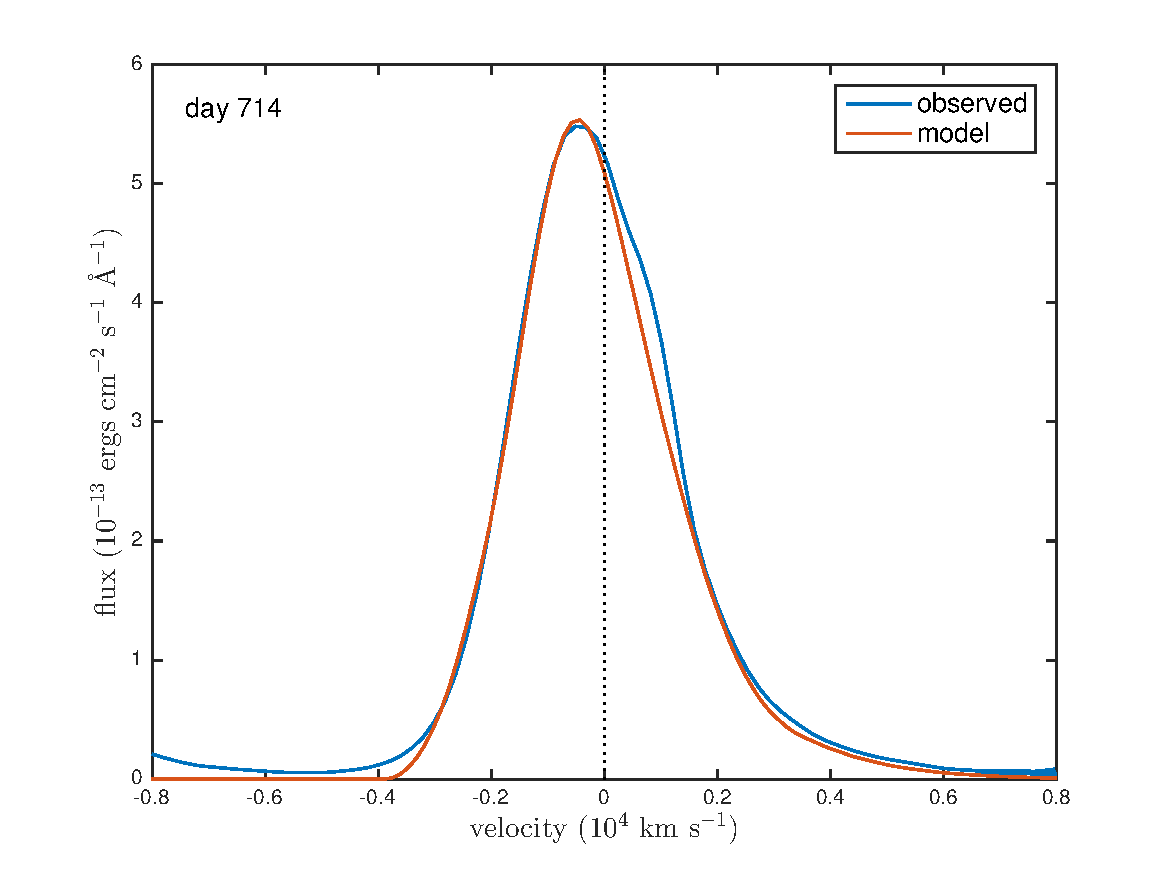
\includegraphics[scale=0.42,clip=true,trim=40 0 40 20]{chapters/chapter5/images/HaOImod_Ha.pdf}
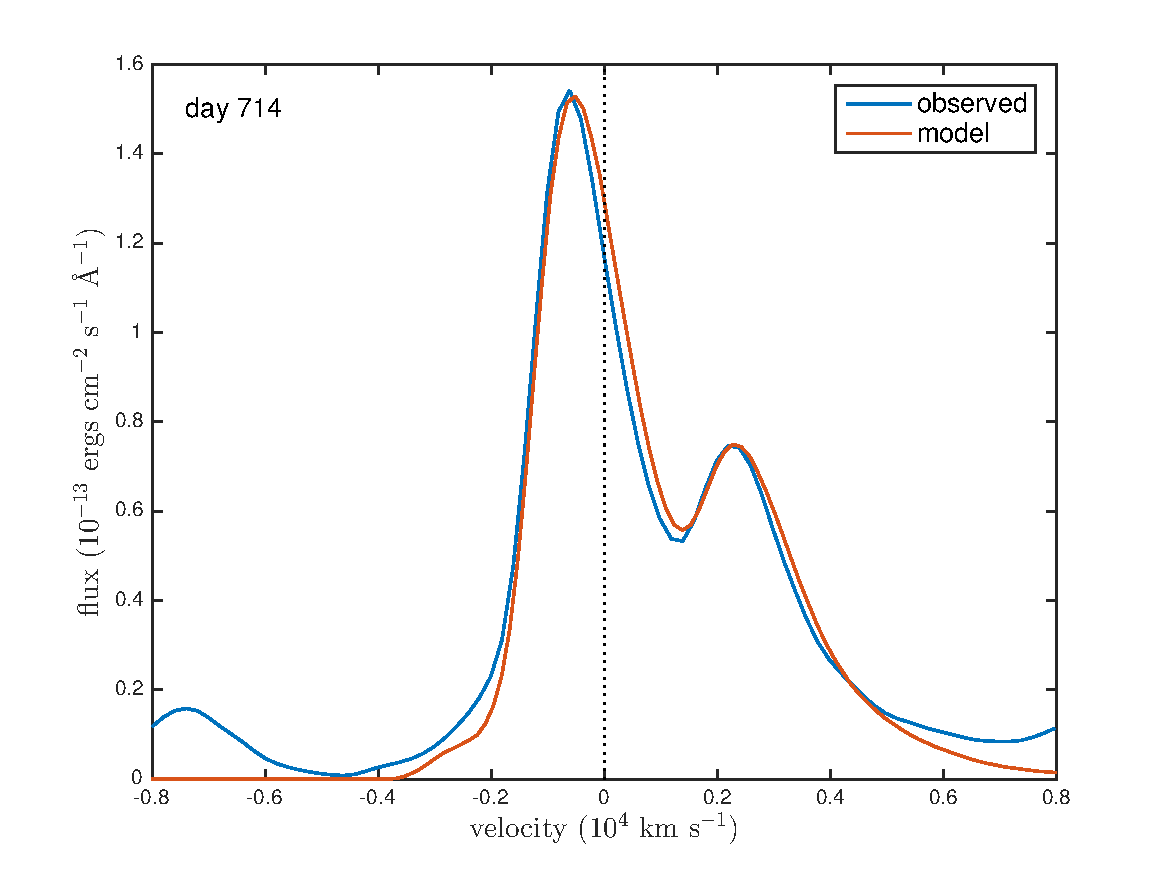
\includegraphics[scale=0.42, clip=true,trim=20 0 40 20]{chapters/chapter5/images/HaOImod_OI.pdf}
\caption{Fits to the H$\alpha$ and [O~{\sc i}]$\lambda$6300,6363~\AA\ lines at day 714 using the more complex dust model described in Section \ref{complex} with a dust mass of  $2.3 \times 10^{-4}$M$_{\odot}$.}
\label{HaOImod}
\end{figure}

In our subsequent analyses, we adopt the values derived from our clumped 
models.  Details of the parameters used are presented in 
Tables \ref{clumped1} and \ref{clumped2} and the fits are presented in Figures 
\ref{Ha} and \ref{d1862_3604}.

\begin{figure*}
\centering

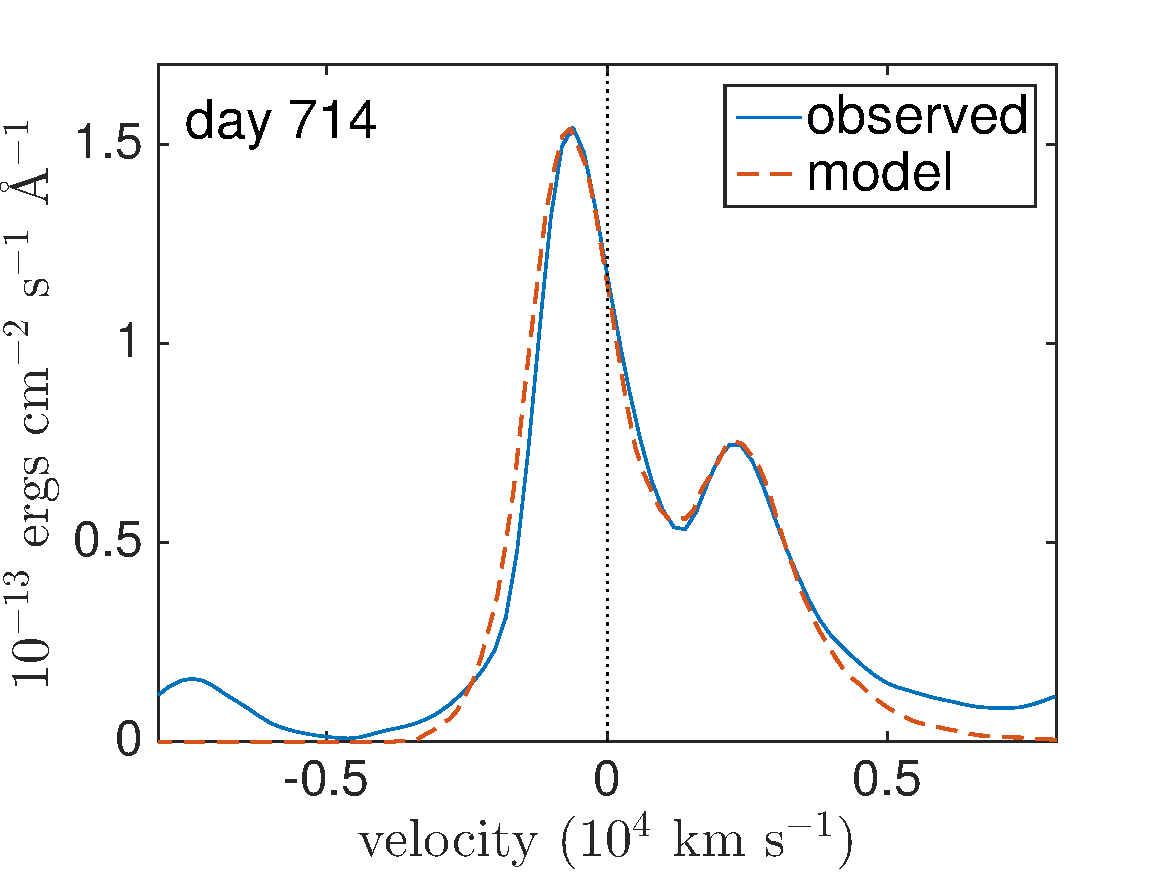
\includegraphics[trim =0 25 0 0,clip=true,scale=0.4]{chapters/chapter5/images/smooth/best_fit/d714OI.pdf}
\hspace{1mm}
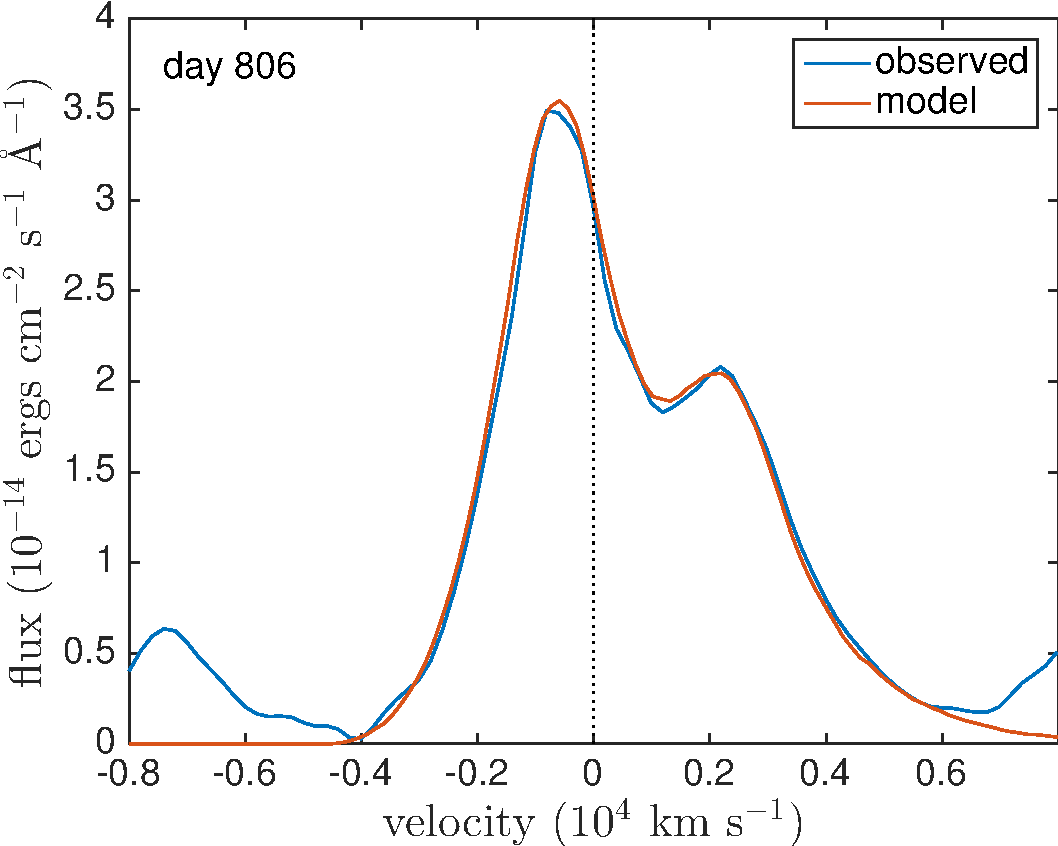
\includegraphics[trim =25 25 0 0,clip=true,scale=0.4]{chapters/chapter5/images/smooth/best_fit/d806OI_ext.pdf}

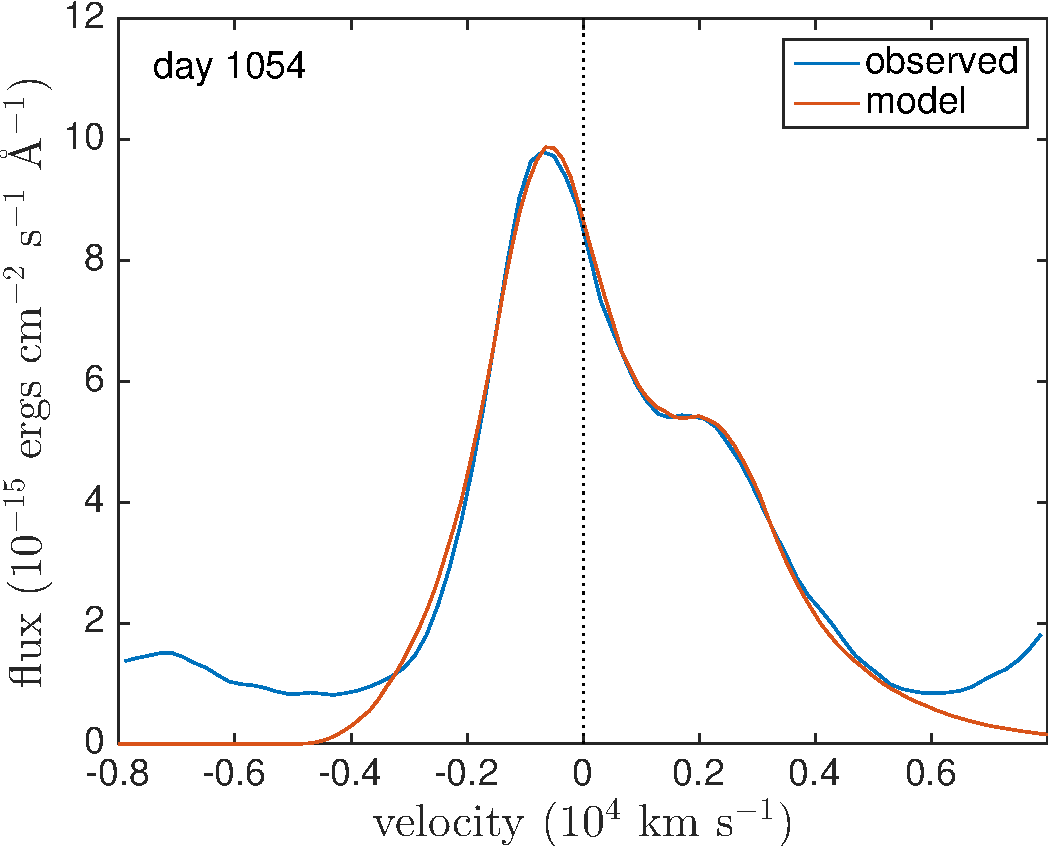
\includegraphics[trim =0 0 0 -20,clip=true,scale=0.4]{chapters/chapter5/images/smooth/best_fit/d1054OI.pdf}
\hspace{1mm}
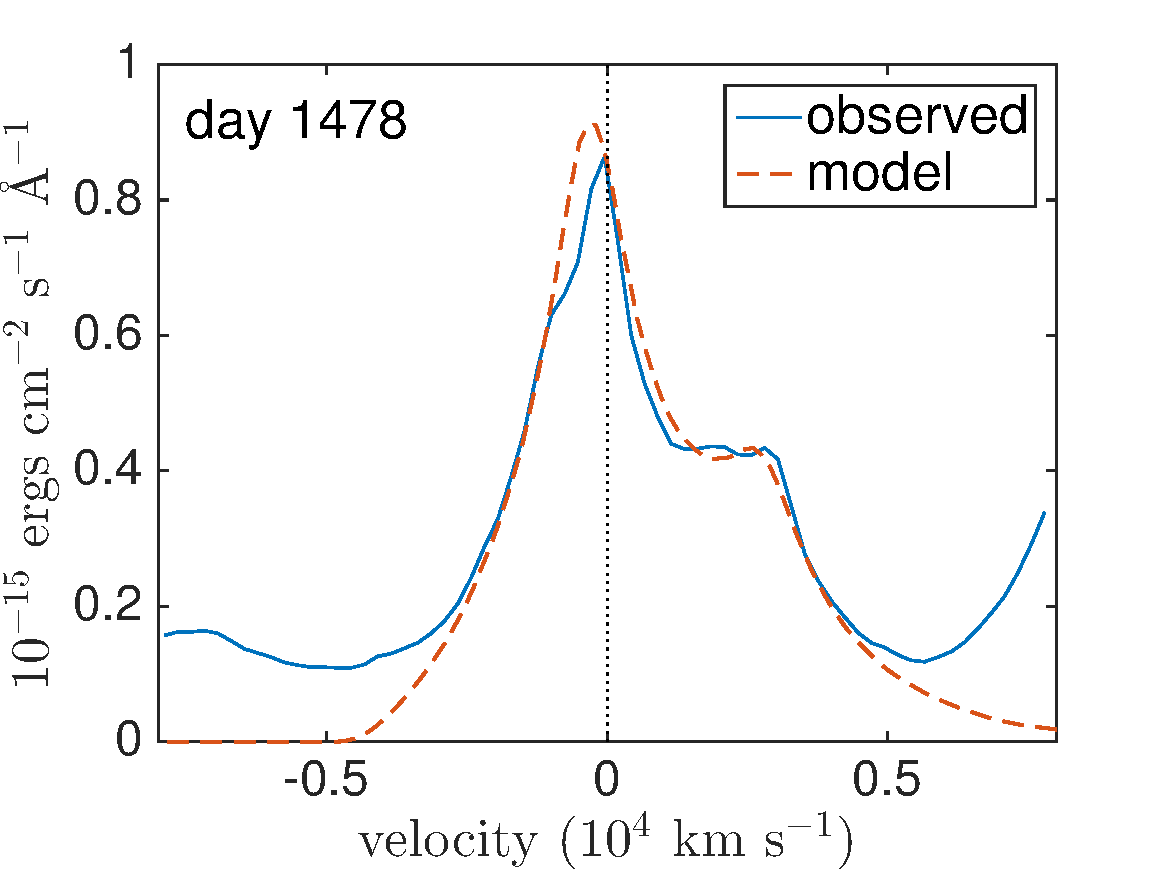
\includegraphics[trim =25 0 0 -20,clip=true,scale=0.4]{chapters/chapter5/images/smooth/best_fit/d1478OI.pdf}


\caption{Best smooth dust fits to the SN~1987A [O~{\sc i}]~$\lambda$6300,6363~\AA\ doublet at days 714, 806, 1054 and 1478 for the parameters detailed in Tables \ref{smooth1}, \ref{clumped1} and \ref{clumped2}.  On the top row are smooth dust fits with amorphous carbon grains of radius $a=0.35 \mu$m.  On the middle and bottom rows are clumped dust fits with amorphous carbon grains of radii $a=0.6 \mu$m and $a=3.5 \mu$m respectively.}
\label{OI_smooth}

\end{figure*}
\begin{figure*}
\centering

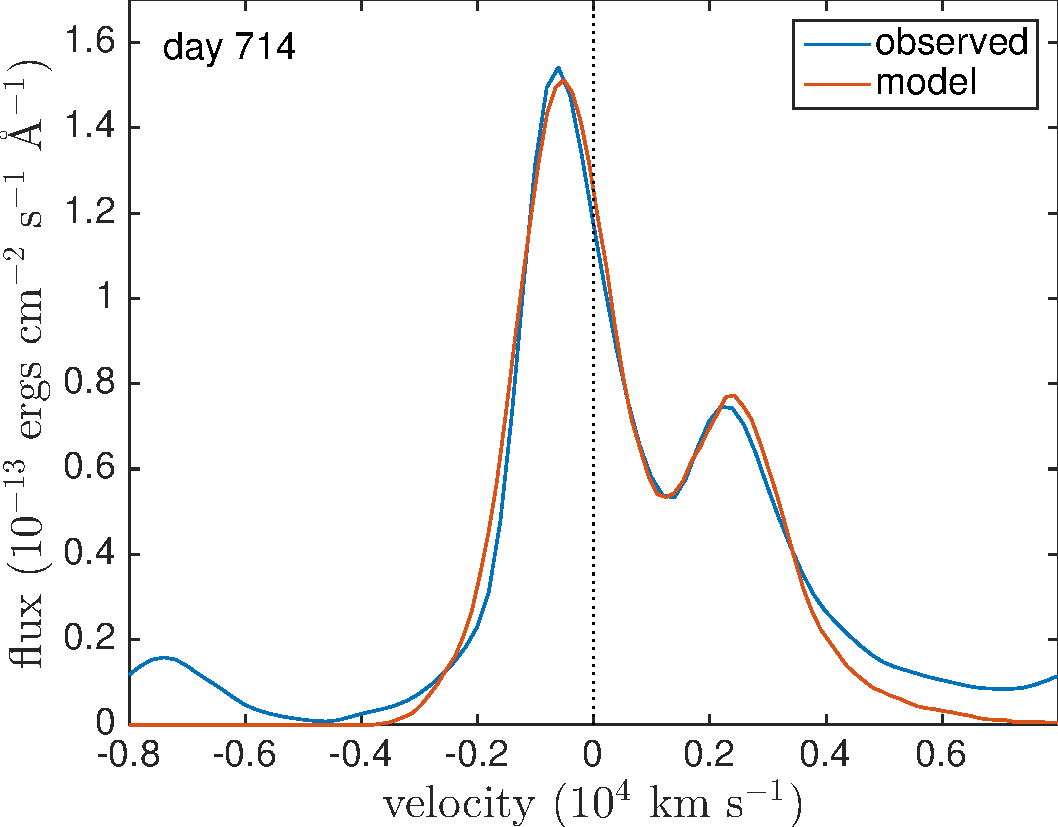
\includegraphics[trim =0 25 0 0,clip=true,scale=0.4]{chapters/chapter5/images/clump_1/best_fit/d714OI_ext.pdf}
\hspace{1mm}
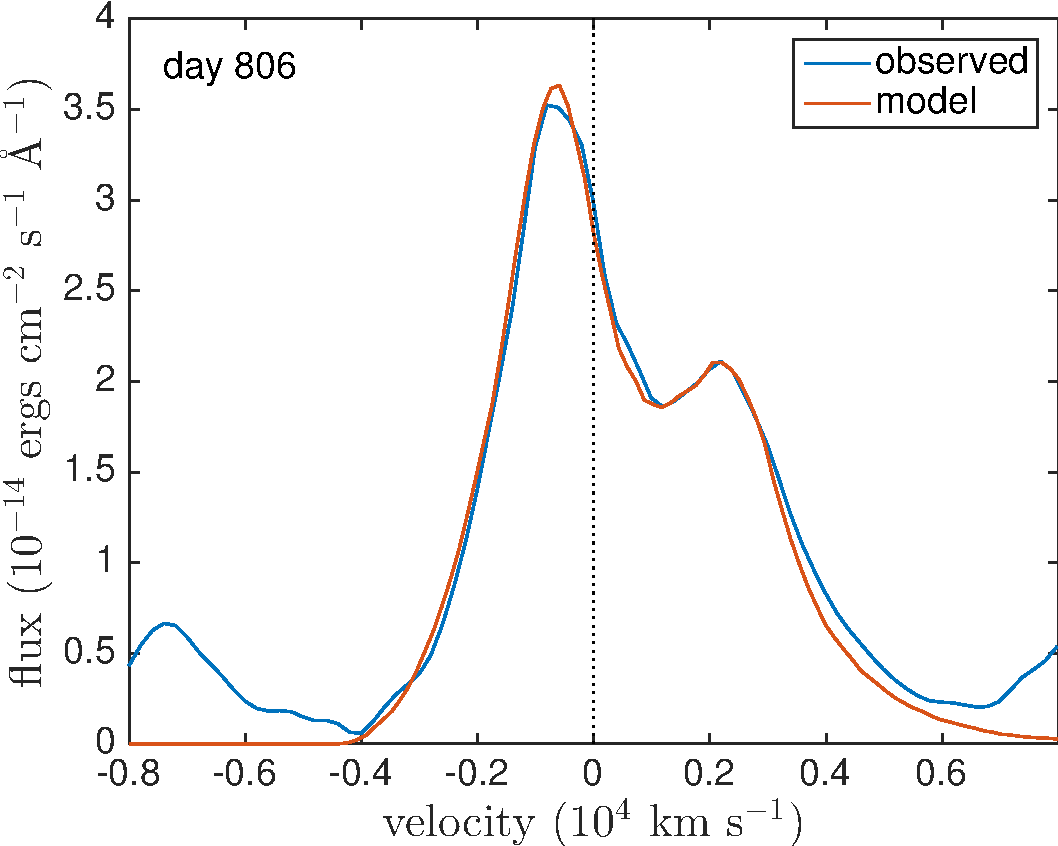
\includegraphics[trim =25 25 0 0,clip=true,scale=0.4]{chapters/chapter5/images/clump_1/best_fit/d806OI_ext.pdf}

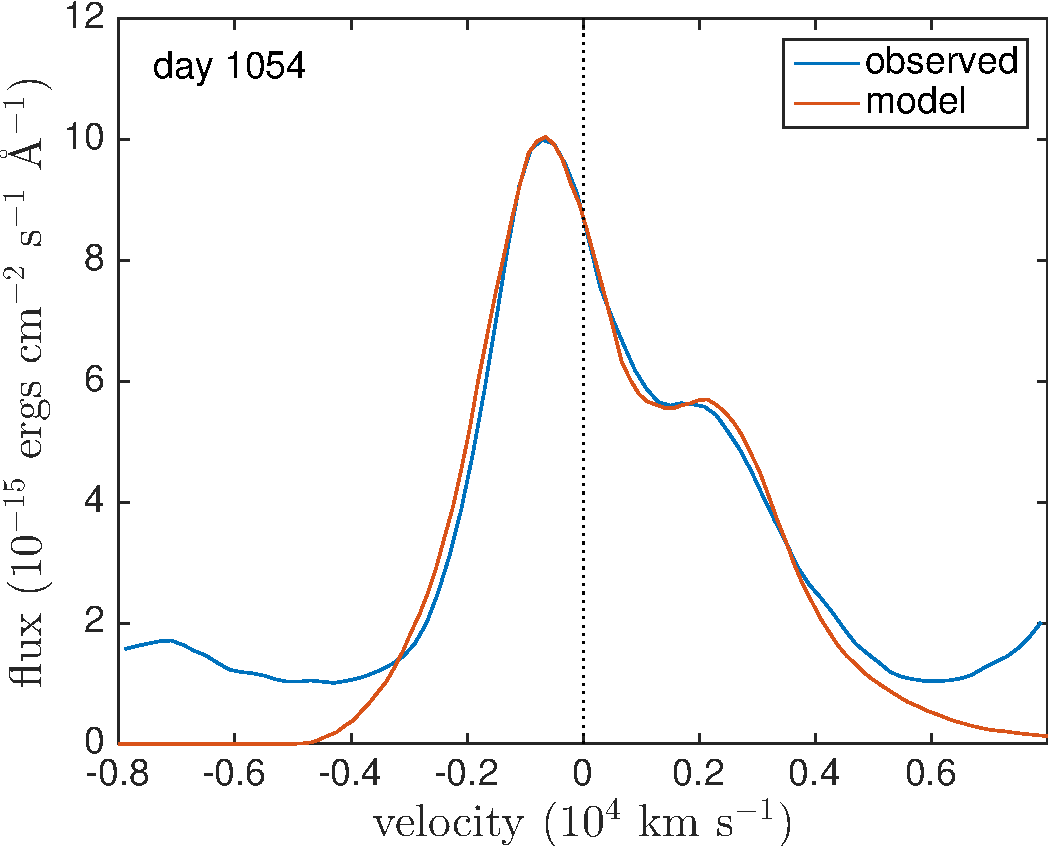
\includegraphics[trim =0 25 0 0,clip=true,scale=0.4]{chapters/chapter5/images/clump_1/best_fit/d1054OI.pdf}
\hspace{1mm}
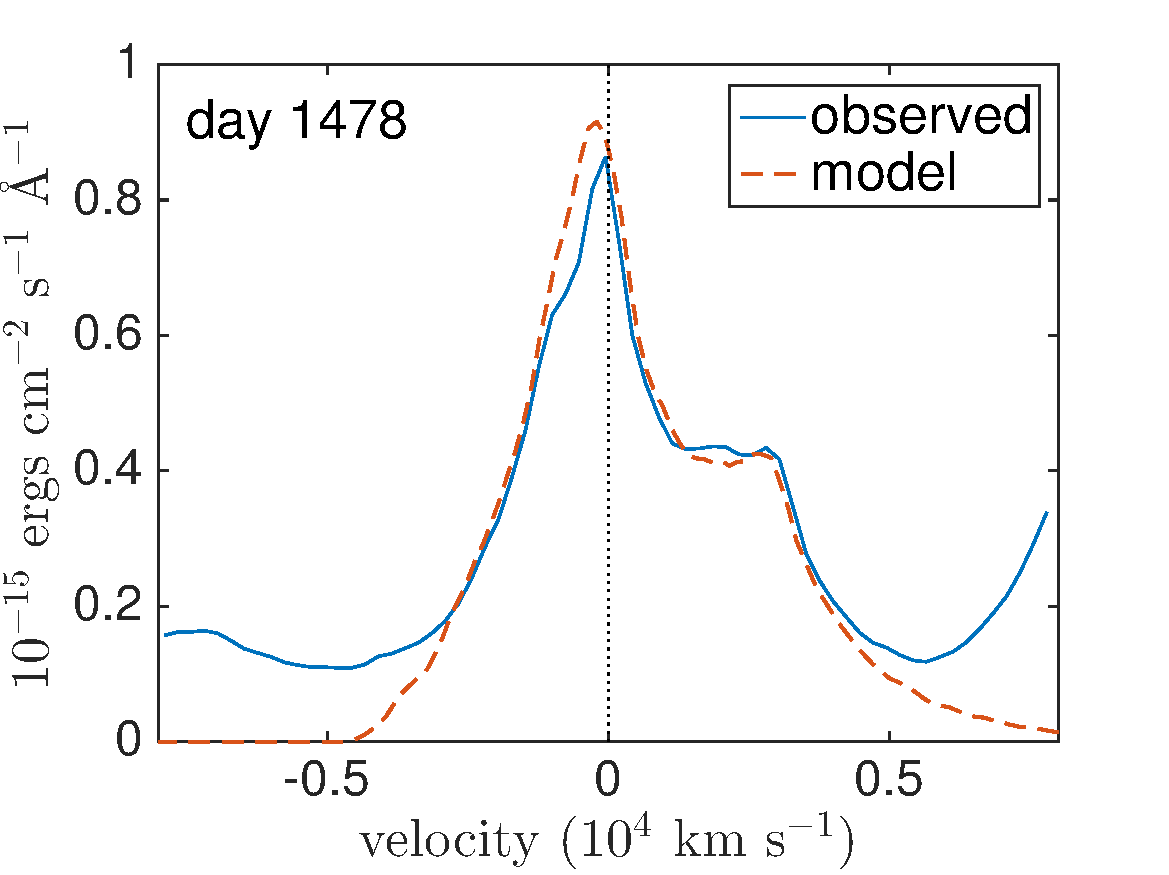
\includegraphics[trim =25 25 0 0,clip=true,scale=0.4]{chapters/chapter5/images/clump_1/best_fit/d1478OI.pdf}

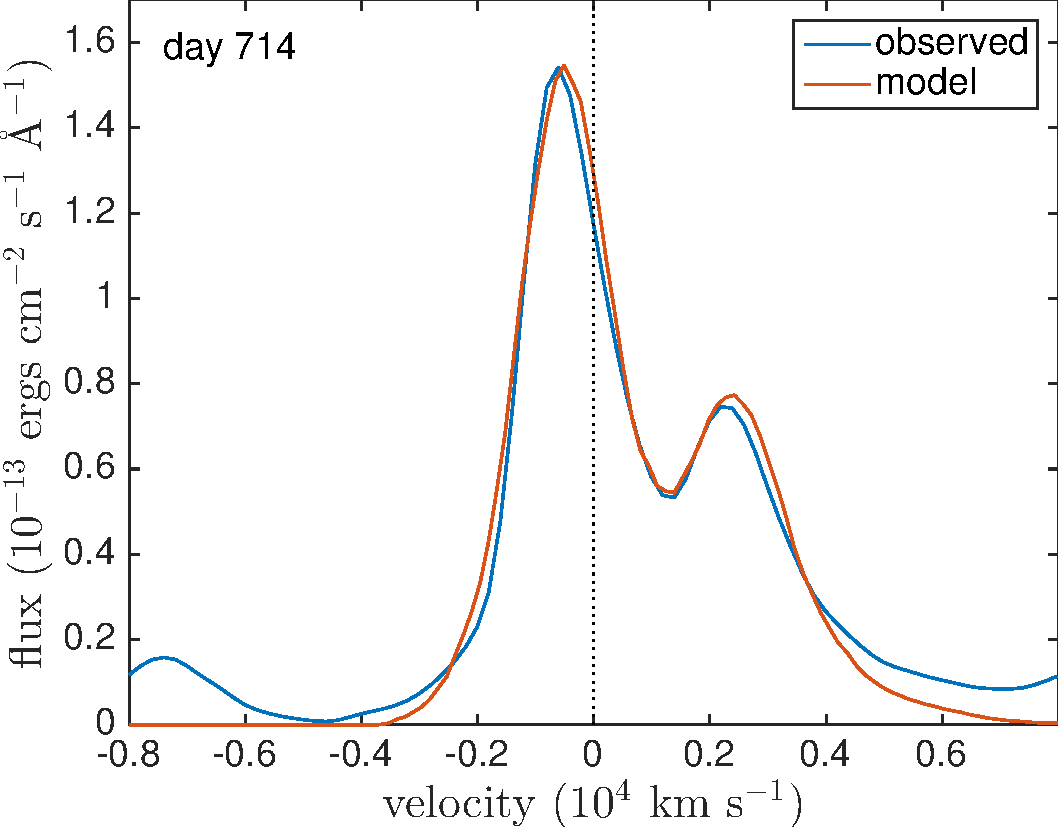
\includegraphics[trim = 0 25 0 0,clip=true,scale=0.4]{chapters/chapter5/images/clump_1/maximum/d714OI_ext.pdf}
\hspace{1mm}
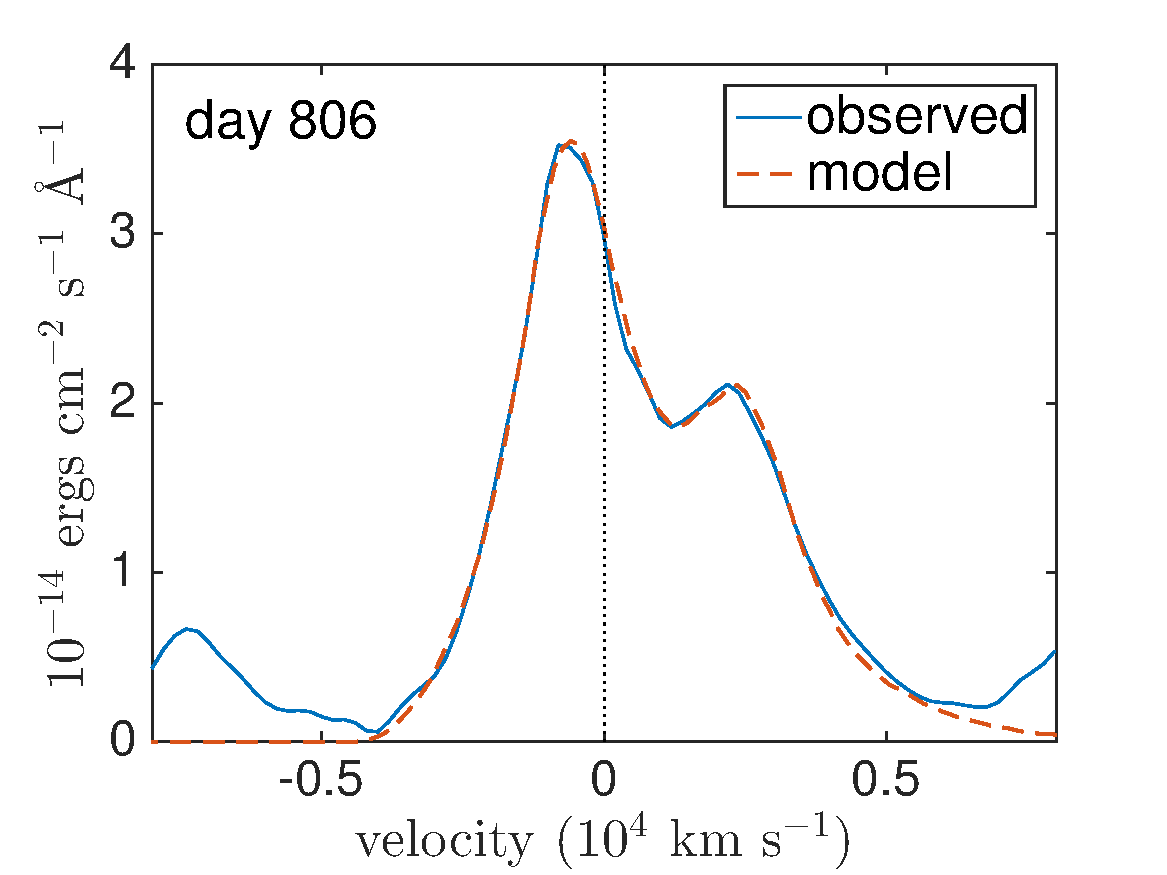
\includegraphics[trim =25 25 0 0,clip=true,scale=0.4]{chapters/chapter5/images/clump_1/maximum/d806OI_ext.pdf}

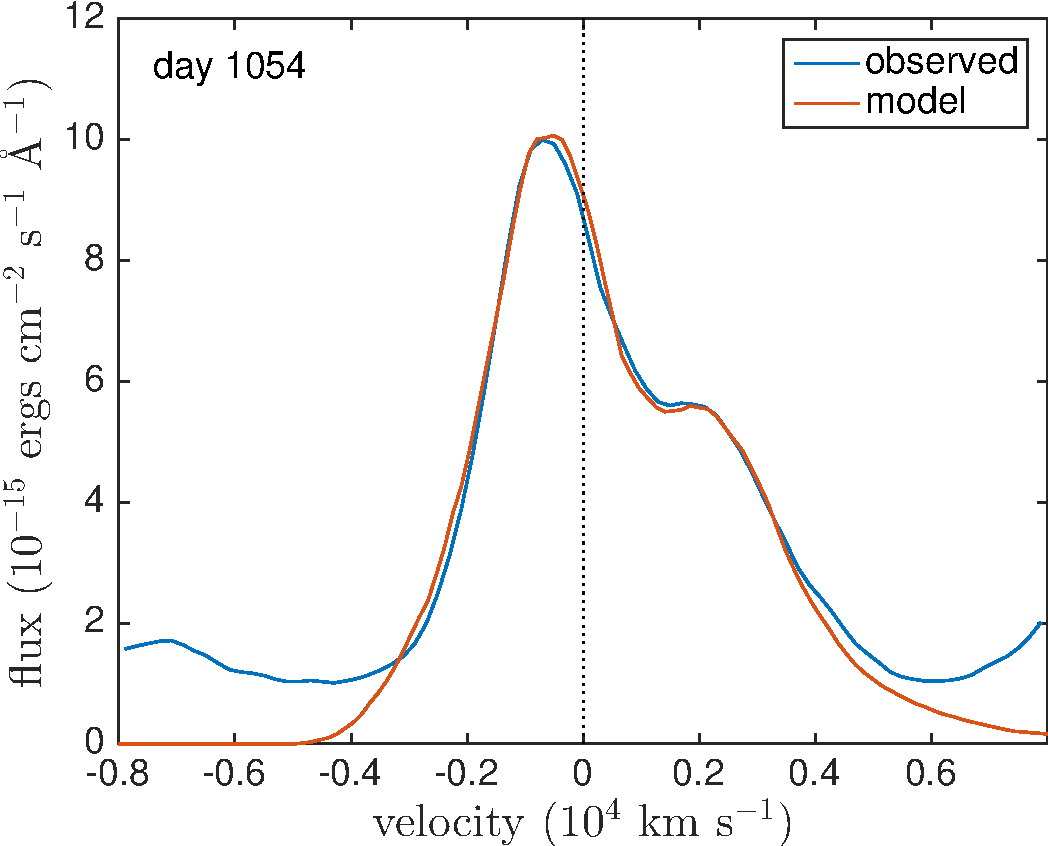
\includegraphics[trim =0 25 0 0,clip=true,scale=0.4]{chapters/chapter5/images/clump_1/maximum/d1054OI.pdf}
\hspace{1mm}
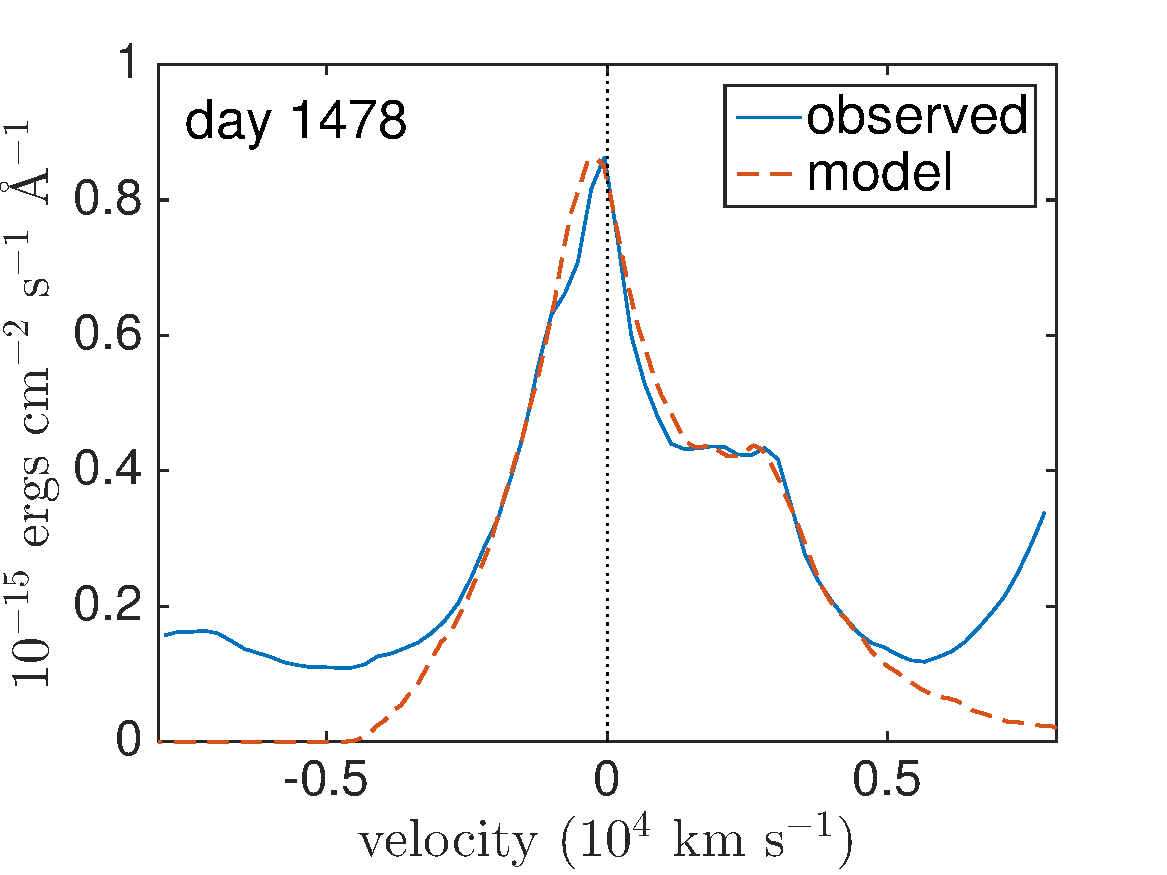
\includegraphics[trim =25 25 0 0,clip=true,scale=0.4]{chapters/chapter5/images/clump_1/maximum/d1478OI_new.pdf}


\caption{Best smooth dust fits to the SN~1987A [O~{\sc i}]~$\lambda$6300,6363~\AA\ doublet at days 714, 806, 1054 and 1478 for the parameters detailed in Tables \ref{smooth1}, \ref{clumped1} and \ref{clumped2}.  On the top row are smooth dust fits with amorphous carbon grains of radius $a=0.35 \mu$m.  On the middle and bottom rows are clumped dust fits with amorphous carbon grains of radii $a=0.6 \mu$m and $a=3.5 \mu$m respectively.}
\label{OI_smooth}

\end{figure*}



\subsection{The effects of clumping}

As in the case of SED radiative transfer models, the dust masses required 
to reproduce the observations in the clumped scenario are considerably 
higher than for the smooth scenario.  The dust masses differ between our 
smooth models for $a=0.35~\mu$m and clumped models for $a=0.6\mu$m by a 
factor of approximately 3.  The dust mass estimates are even larger when
comparing clumped $a=0.6~\mu$m models to clumped $a=3.5~\mu$m models at 
later epochs. This does not take into account the increase in grain radius 
between the two cases however.  This increase accounts for a reasonable 
fraction of this difference. We estimate the effects of clumping alone to 
increase the required dust mass by a factor of approximately 1.5-2.0 from 
the smooth case.


\subsection{More complex models}
\label{complex}

Where blue-shifted lines are observed in the spectra of CCSNe it is often the case that the Balmer lines of HI are less affected than the [O~{\sc i}] lines \citep{Milisavljevic2012}.  This may be due to a difference in the location or distribution of the emitting elements; if the neutral hydrogen was diffusely distributed throughout the envelope but the oxygen was co-located with the dust in the core and in clumps then this could result in [O~{\sc i}] emission undergoing greater attenuation than H$\alpha$.  This geometry would be in line with previous models of SN~1987A that suggested that the dust-forming regions are likely to include those which are oxygen-rich \citep{Kozma1998a}.  Clearly, any model of dust formation in the ejecta of a CCSN must consistently reproduce all of the line profiles at a given epoch.  The models presented in this paper thus far have coupled the gas and dust distributions for a fixed clump volume filling factor and clump size.  The H$\alpha$ and [O~{\sc i}] models therefore require different dust masses with the [O~{\sc i}] models usually requiring a dust mass $\sim4$ times larger than the H$\alpha$ models. 

We now present a model that reconciles this difference by additionally varying the clump filling factor, clump size and emissivity distribution.  We assume that neutral hydrogen is likely diffuse throughout the ejecta and so maintains a smoothly distributed power-law emissivity distribution between $R_{in}$ and $R_{out}$ for H$\alpha$.  However, we now assume that dust mostly forms in dense regions of high metallicity and so restrict the [O~{\sc i}]$\lambda$6300,6363~\AA\ emission to originate largely from the dusty clumps with only a small fraction emitted from the inter-clump medium.  As previously discussed, the greater the covering factor of the dust the greater the albedo required in order to reproduce the H$\alpha$ red scattering wing. In order to obtain both the strong blue-shifting of the [O~{\sc i}] line and the extended red scattering wing observed in H$\alpha$ a small number of dense clumps were required along with a small mass of diffusely distributed highly scattering dust in the inter-clump medium.


In order to fit both line profiles simultaneously we required a very high albedo ($\omega > 0.8$) that demanded the inclusion of some fraction of silicate dust. Amorphous carbon grains alone are incapable of producing this level of scattering for any grain size.  We adopted a grain radius of $a=0.6\mu$m, the same as that used in our initial clumped models and we varied the relative proportions of amorphous carbon and MgSiO$_3$ in order to achieve the necessary albedo.  The adopted grain densities were $\rho_c=1.85$~g~cm$^{-3}$ for amorphous carbon grains and $\rho_s = 2.71$~g~cm$^{-3}$ for MgSiO$_3$.  The resulting dust model for day 714 used 75\% MgSiO$_3$ and 25\% amorphous carbon by cross-sectional area with a volume filing factor $f_V=0.1$ and a clump size $R_{out}/5$.  90\% of the dust mass was located in clumps with the remaining 10\% emitted smoothly between $R_{in}$ and $R_{out}$ according to a power law $\rho \propto r$. Clumps were distributed stochastically with probability $\propto r^{-8}$ compared to $r^{-2.7}$ in our standard models discussed earlier. Equal numbers of [O~{\sc i}] packets were emitted from each clump. H$\alpha$ was distributed smoothly according to a density power law $\rho(r) \propto r^{-1.3}$.  $R_{out}$ was the same for all components (i.e. clumped dust, diffuse dust, [O~{\sc i}] emission and H$\alpha$ emission) and was calculated using a maximum velocity of 3250~km~s$^{-1}$.  The inner radius was $R_{in} = 0.07 R_{out}$ for all components except the smooth H$\alpha$ emission which was emitted between $R_{in}=0.25R_{out}$ and $R_{out}$.  

The total dust mass used was $M_{dust}=2.3 \times 10^{-4}$~M$_{\odot}$.  This dust mass is very similar to that derived from our original clumped models of [O~{\sc i}] using amorphous carbon grains of radius $a=0.6\mu$m.  The slight increase over our amorphous carbon dust mass of $1.5 \times 10^{-4}$~M$_{\odot}$ is largely due to the higher grain density of MgSiO$_3$.  At this grain radius amorphous carbon and MgSiO$_3$ have similar extinction efficiencies and so the change in species and geometry does not substantially alter the dust mass. We therefore adopt the [O~{\sc i}] dust masses in our further analyses and consider the differences in our derived dust masses between H$\alpha$ and [O~{\sc i}] to be the result of the clumped emission of [O~{\sc i}].


Fits to both the [O~{\sc i}]$\lambda$6300,6363~\AA\ and H$\alpha$ lines for day 714 using these parameters are presented in Figure \ref{HaOImod}.

%%%%%%%ADDITIONAL CONTENT%%%%%%%%%%%%%%%%%

\subsection{The effect of a grain size distribution}
\label{gs_distn}

It is important to consider the potential effect on the dust mass of 
modelling a grain size distribution instead of a single grain size.  For a 
grain size distribution the overall extinction cross section, $C_{ext}$, 
at a given wavelength is

\begin{equation}
 C_{ext}=\int^{a_{max}}_{a_{min}} Q_{ext}(a) n(a) \pi a^2 da 
 \end{equation}

where $Q_{ext}(a)$ is the extinction efficiency for a grain size $a$ and 
$n(a)$ is the number of grains with size $a$. The overall extinction 
efficiency is then

\begin{equation}
 Q_{ext} = \frac{C_{ext}}{ \int^{a_{max}}_{a_{min}} n(a) \pi a^2 da} 
 \end{equation}
 
The scattering cross-section $Q_{sca}$ is similarly calculated.  As a 
result of these calculations, there is rarely a single grain size that has 
the same albedo and extinction efficiency as a size distribution.  
Modelling a size distribution may therefore alter the deduced dust mass.  
Since the models are only sensitive to the overall optical depth and 
albedo, it is not possible to deduce the grain size range or distribution 
and only single grain sizes are investigated (as presented above).

Whilst this apparently limits the scope of the results, it is useful to 
consider the extent to which different grain size distributions would 
alter the derived dust masses.  By considering a number of grain radius 
ranges and adopting a power law distribution with a variable exponent, we 
may gain some insight into the effects of adopting a distribution rather 
than a single size.  As discussed in Section \ref{smooth_models}, a classical MRN power law ($n(a) \propto 
a^{-3.5}$) with a wide grain radius range ($a_{min} = 0.001~\mu$m to 
$a_{max} = 4.0~\mu$m) the derived albedo is much too small to reproduce 
the required wing seen at early epochs.  We therefore adopt an approach 
whereby, for a number of grain size ranges, we adjust the exponent of the 
distribution until the overall albedo is the same as that seen for the 
best fitting single grain radius for the clumped distributions.  We may 
then approximately calculate the required dust mass as

\begin{equation}
\label{distn_conv}
M_{d}= \frac{M_s Q_{ext,s}(a_s)}{a_s} \times \frac{\int^{a_{max}}_{a_{min}} n(a) a^3 da}{\int^{a_{max}}_{a_{min}} Q_{ext}(a) n(a) a^2 da}
\end{equation}

where the subscript $s$ represents the single grain size quantities and 
the $d$ subscript represents quantities for the grain size distribution.


We calculate the required dust masses for the clumped H$\alpha$ model on 
day 714 for a selection of distributions with varying $a_{min}$.  These 
are presented in Table \ref{tb_distn}.  It can be seen that in all cases, 
a larger dust mass is required for grain size distributions in order to reproduce the same profile as a 
single grain size.  The conversion factors presented in the table are 
valid for any model with grain size $a=0.6~\mu$m and may therefore also be 
applied to the models for day 806.  We repeated the process for 
$a=3.5~\mu$m but found that, in order to reproduce the required albedo, the 
distribution had to be heavily weighted towards the larger grains and that 
the value of $a_{min}$ had no effect on the required dust mass.  
Increasing the value of $a_{min}$ to larger values ($>2~\mu$m) does not 
have a significant effect either.  This is because both extinction 
efficiency and albedo tend to a constant value with increasing grain 
radius and the adoption of different grain size ranges and distributions 
above a certain threshold results in only insignificant variations in 
these quantities.
\setlength{\tabcolsep}{12pt}
\begin{table}
	%\begin{minipage}{180mm}
	\caption{Dust masses for day 714 clumped models of the H$\alpha$ 
line using different grain size distributions and 100\% amorphous carbon. The final column shows the factor of increase over the dust mass for the single size model ($M=7 \times 10^{-5} M_{\odot}$ with $a=0.6~\mu$m) and $p$ is the exponent of the grain size distribution $n(a) \propto a^{-p}$.}
	\label{tb_distn}
	\begin{center}
  	\begin{tabular}{@{} ccccc @{}}
    	\hline
$a_{min}$ & $a_{max}$ & $p$ & $M$ & $M/M_{0.6}$  \\%& $Q_{ext}$ \\
($\mu$m) & ($\mu$m) & & ($M_{\odot}$) & \\
\hline
0.001 & 4.0 & 2.45 & 1.93 $\times 10^{-4}$ & 2.76 \\%& 2.13 \\
0.01 & 4.0 & 2.45 & 1.93 $\times 10^{-4}$ & 2.76 \\%& 2.32 \\
0.05 & 4.0 & 2.52 & 1.84 $\times 10^{-4}$ & 2.62 \\%& 2.44 \\
0.1 & 4.0 & 2.72 & 1.61 $\times 10^{-4}$ & 2.3\\ %& 2.53 \\
0.5 & 4.0 & 8.20 & 7.23 $\times 10^{-5}$ & 1.03 \\%& 2.61 \\

    \hline
  \end{tabular}
  \end{center}
%\end{minipage}
\end{table}
\setlength{\tabcolsep}{7pt}


We conclude that if a distribution of grain sizes is indeed present, the 
deduced single size dust masses are likely to under-estimate the true mass 
of newly formed dust.

\subsection{The effect of different grain species}
\label{species}

In our analyses so far we have considered only amorphous carbon as the 
species of interest.  This was motivated by previously published early epoch optical 
and IR SED analyses that found that the silicate mass fraction must be  limited to $\leq$15\% (\citet{Ercolano2007}, W15).  The recent suggestion by 
\citet{Dwek2015} that large masses of the  glassy silicate MgSiO$_3$ 
may have formed at early epochs is discussed further in the next 
subsection.  The parameters that affect the quantity of dust required by 
our models are the mean albedo and optical depth of the dust.  There could 
be multiple combinations of grain species and sizes that result in a good 
fit to the data.

We can evaluate the required change in dust mass when a medium of 100\% 
silicates is used instead of amorphous carbon. Using the astronomical 
silicate optical constants of \cite{Draine1984}, which are `dirtier' (with 
lower albedos) than the glassy pure MgSiO$_3$ sample of \citet{Jager2003}. 
In a similar manner to the approach detailed in Section \ref{gs_distn}, we 
can calculate the mass of DL silicate that gives a fit equivalent to that 
for a single carbon grain radius.  We consider the albedo for the grain 
radius needed for the best fit amorphous carbon model, calculate the 
equivalent grain radius for DL silicate that gives the same albedo and 
then calculate a new dust mass by allowing for the change in the 
extinction cross-section:

\begin{equation}
M_{sil} = M_{amc} \Big( \frac{Q_{amc}}{Q_{sil}} \Big) \Big(\frac{a_{sil}}{a_{amc}}\Big) \Big(\frac{\rho_{sil}}{\rho_{amC}}\Big)
\end{equation}

Because of the nature of the variation of albedo with grain radius for the 
\citet{Draine1984} astronomical silicate (see Figure \ref{albedo_grain}), 
there is often more than one silicate grain radius that will give rise to 
the same albedo at a given wavelength.  Some of the possibilities and the 
resulting mass conversion factors are given in Table \ref{tb_sil}.  For 
our best fitting amorphous carbon models with $a=0.6~\mu$m (the first two 
entries in Table \ref{tb_sil}), using any fraction of silicates with 
either $a=0.6~\mu$m or $a=3.5~\mu$m would increase the dust mass.  
However, 
for the case of an amorphous carbon grain radius of $a=3.5~\mu$m (the last 
three entries), using silicate dust would reduce the dust mass by a factor 
of about two relative to our amorphous carbon values.

\begin{table}
	%\begin{minipage}{180mm}
	\caption{Dust mass conversion factors for single size models using  
grains of 100\% Zubko BE amorphous carbon or 100\% Draine \& Lee silicate 
at $\lambda \sim 656$~nm. $f$ is the factor by which the dust mass 
changes on going from amorphous carbon to silicates.}
	\label{tb_sil}
	\begin{center}
  	\begin{tabular}{@{} cccccccc @{}}
    	\hline
	\multicolumn{3}{c}{\textit{carbon}} && \multicolumn{3}{c}{\textit{silicates}} & \\
$a$ &$\omega$ &  $Q_{ext}$ & &$a$&$\omega$ & $Q_{ext}$ & M$_{sil}$/M$_{amc}$ \\
($\mu$m) &&&&($\mu$m)\\
\hline
0.6 & 0.56 & 2.61 & &0.0583 & 0.58 &0.08 & 5.37 \\
0.6 &0.56 & 2.61 & &4.00 & 0.56 & 2.18 & 13.0 \\
 \\
3.5 & 0.62 &2.21 & &0.0641 & 0.64 & 0.10 & 0.65 \\
3.5 & 0.62 &2.21 & &1.020 & 0.63 & 2.15 & 0.49 \\
3.5 & 0.62 & 2.21 & &1.376 & 0.62 & 2.35 & 0.61 \\


    \hline
  \end{tabular}
  \end{center}
%\end{minipage}
\end{table}

\begin{landscape}
\begin{figure*}
\centering
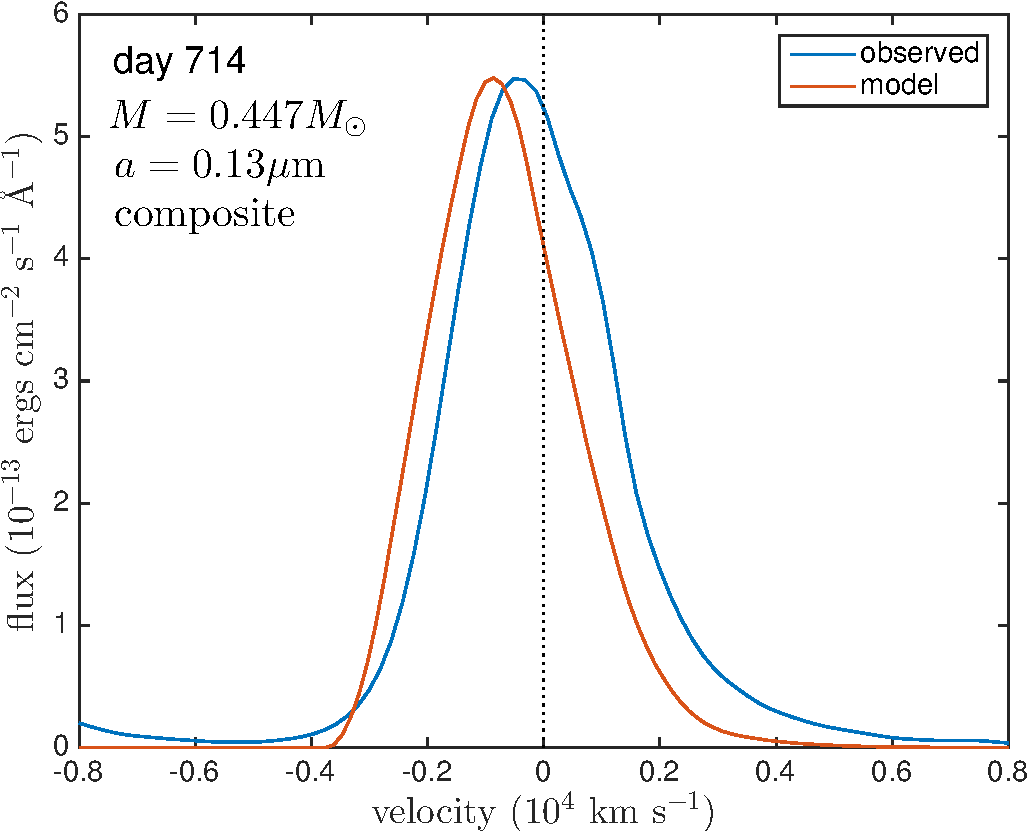
\includegraphics[trim =0 20 0 0,clip=true,scale=0.33]{chapters/chapter5/images/silicates_take2/composite_Dwek_Ha.pdf}
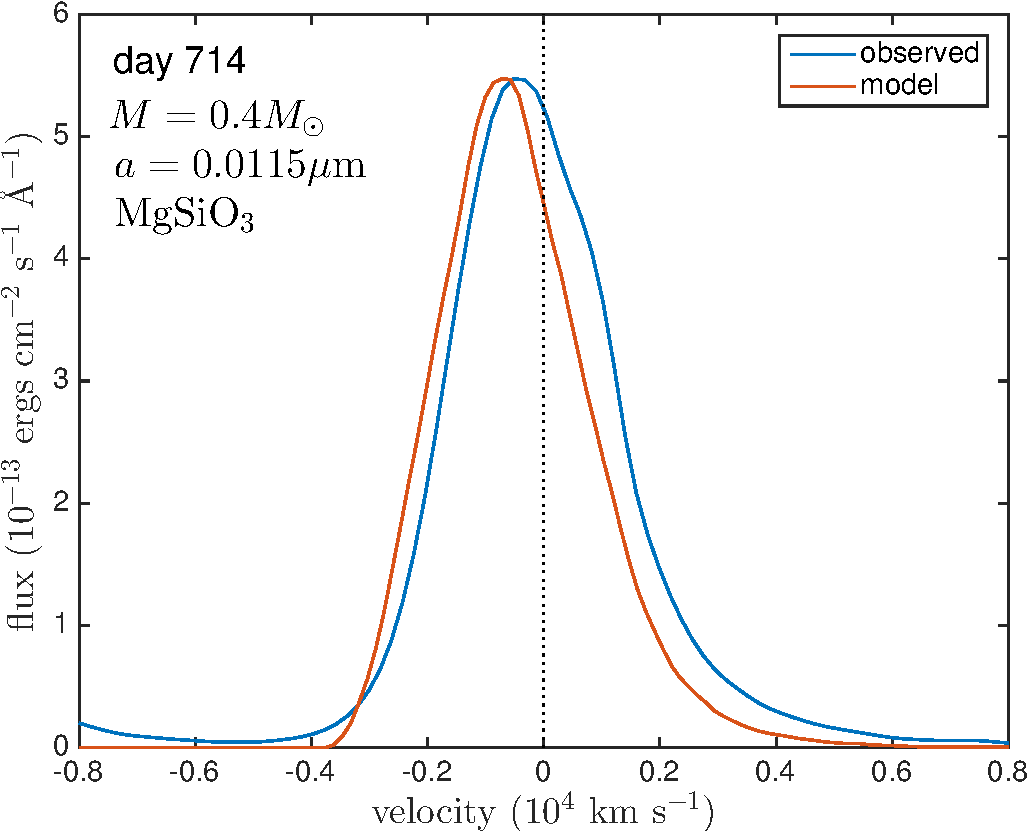
\includegraphics[trim =24 20 0 0,clip=true,scale=0.33]{chapters/chapter5/images/silicates_take2/MgSiO3_Dwek_Ha.pdf}
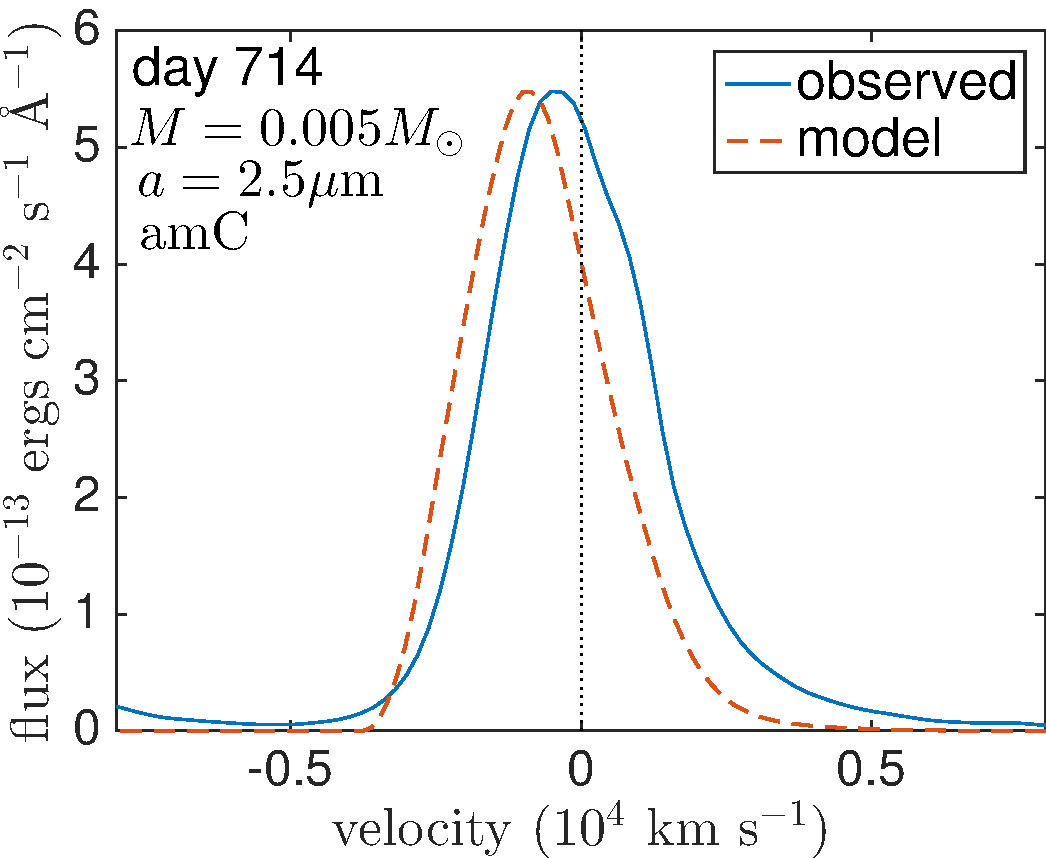
\includegraphics[trim =24 20 0 0,clip=true,scale=0.33]{chapters/chapter5/images/silicates_take2/AmC_Dwek_Ha.pdf}
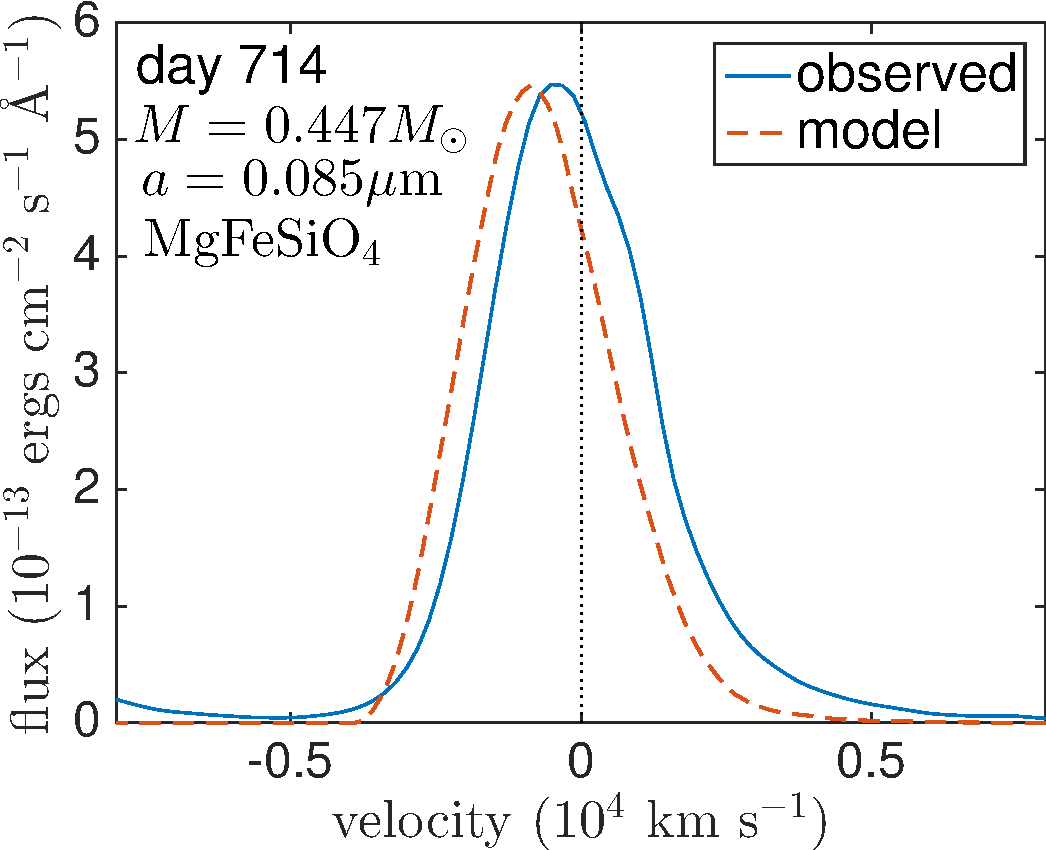
\includegraphics[trim =24 20 0 0,clip=true,scale=0.33]{chapters/chapter5/images/silicates_take2/MgFeSiO4_Dwek_Ha.pdf}

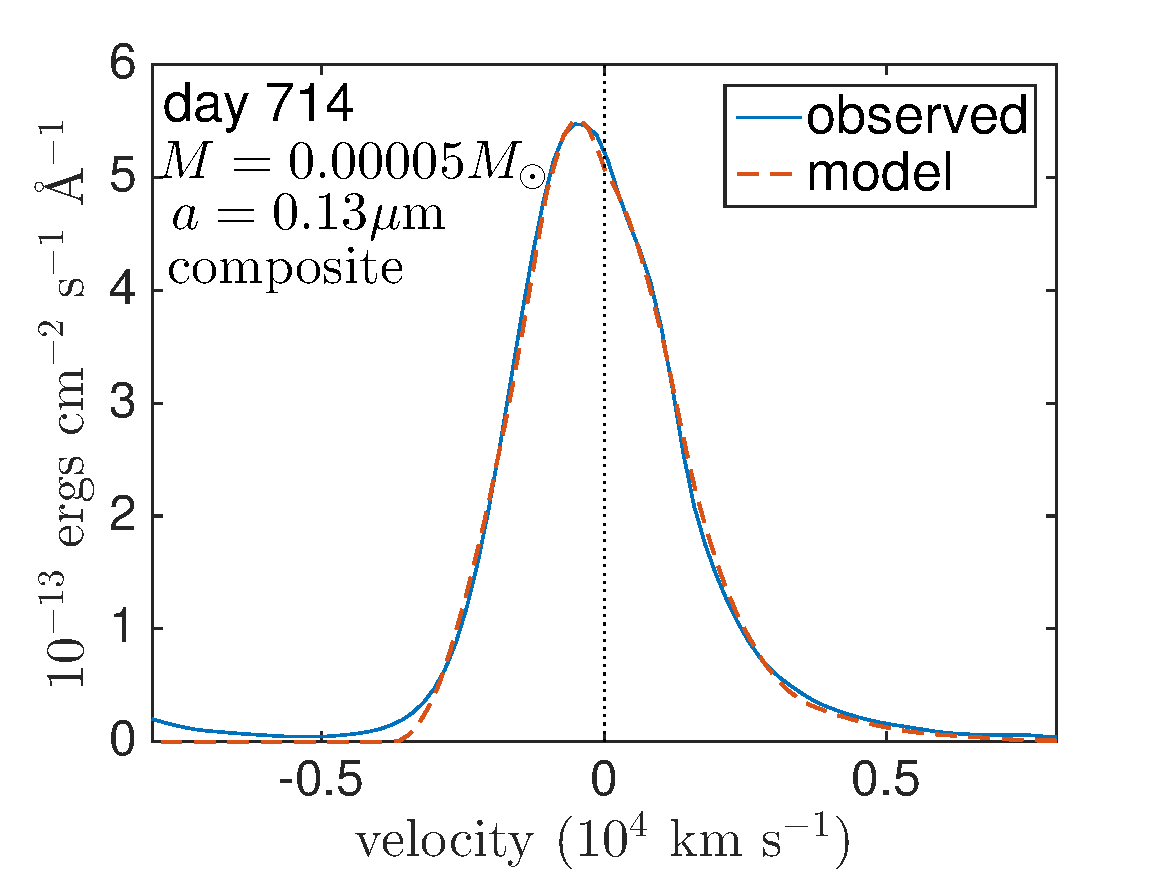
\includegraphics[trim =0 0 0 -10,clip=true,scale=0.33]{chapters/chapter5/images/silicates_take2/composite_bestfit_Ha.pdf}
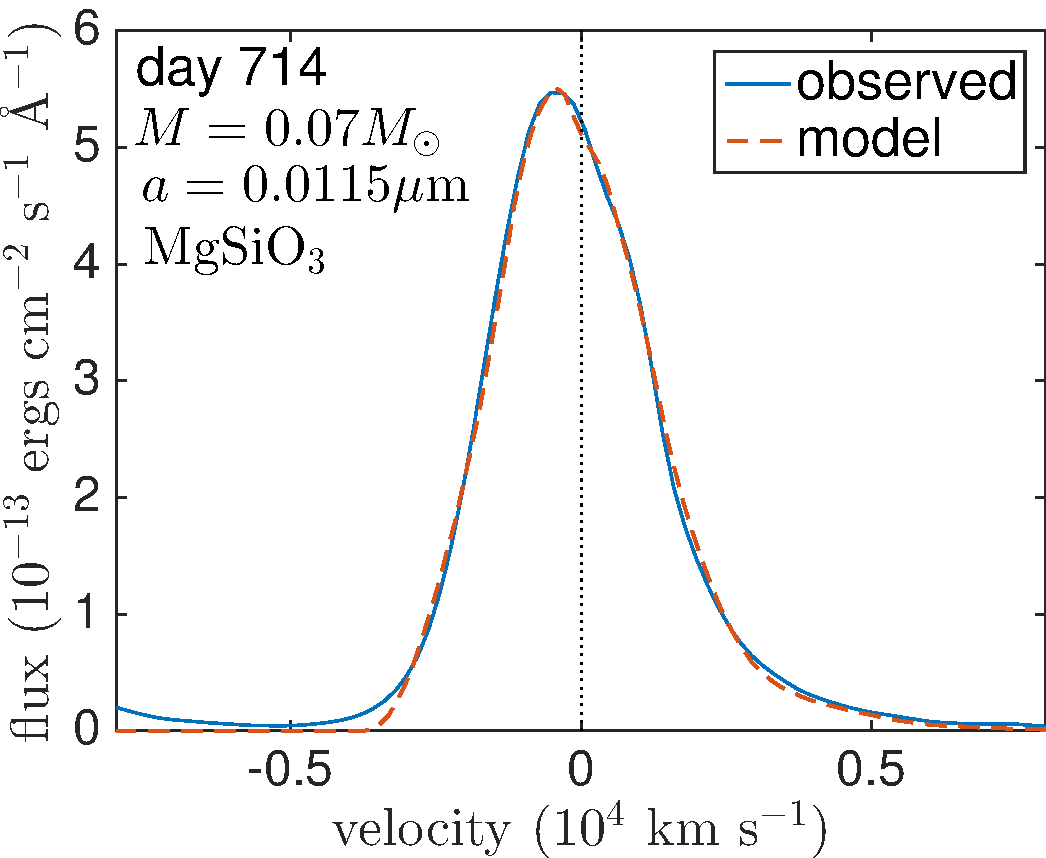
\includegraphics[trim =24 0 0 -10,clip=true,scale=0.33]{chapters/chapter5/images/silicates_take2/MgSiO3_bestfit_Ha.pdf}
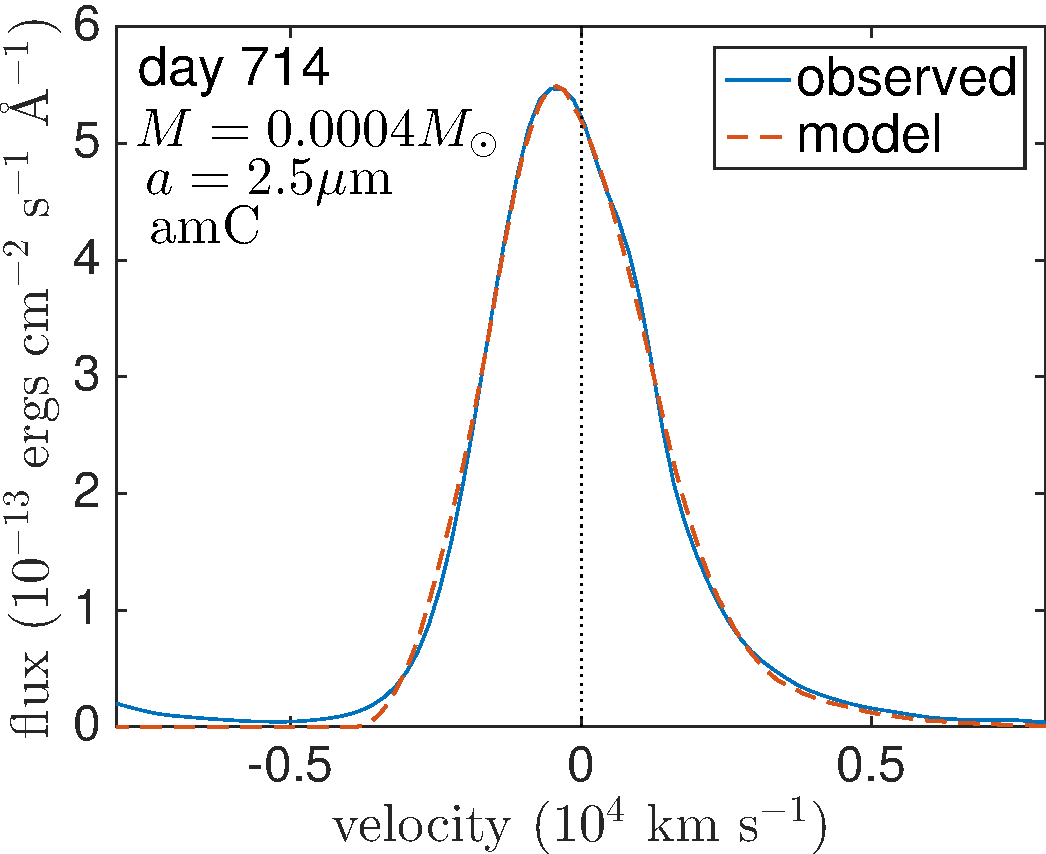
\includegraphics[trim =24 0 0 -10,clip=true,scale=0.33]{chapters/chapter5/images/silicates_take2/AmC_bestfit_Ha.pdf}
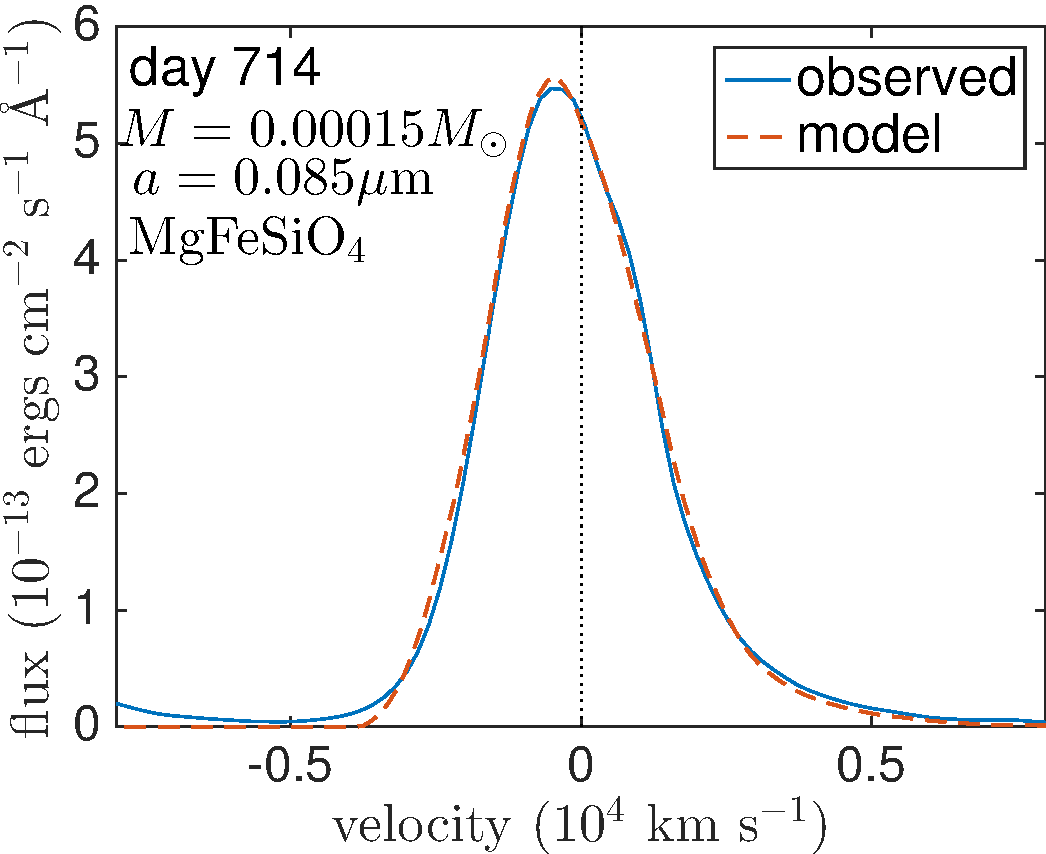
\includegraphics[trim =24 0 0 -10,clip=true,scale=0.33]{chapters/chapter5/images/silicates_take2/MgFeSiO4_bestfit_Ha.pdf}
\caption{H$\alpha$ models using different grain species and dust masses.   
Models for the dust masses presented by \citet{Dwek2015} are on the top and models 
using our minimum required dust masses are on the bottom.  From left to 
right the dust species are composite grains (82\% MgSiO$_3$ and 18\% 
amorphous carbon by volume), pure MgSiO$_3$, pure amorphous carbon and pure 
MgFeSiO$_4$. A density distribution with $\beta=2.3$ was adopted with a 
filling factor $f=0.09$ and an effective clump radius 
$R_{eff}/R_{out}=0.044$.  All other parameters are the same as in Table 
\ref{clumped1}.}
\label{Dwek_models_Ha}
\end{figure*}
\end{landscape}

\subsection{Modelling large masses of dust at early epochs: comparison 
with the results of \citet{Dwek2015}}
\label{dwek}

In a recent analysis of infrared SED data, \citet{Dwek2015} (hereafter 
DA15) suggested that it may be possible for a large mass (0.4~M$_\odot$) of 
MgSiO$_3$ silicate dust to have been present in SN~1987A even at 
relatively early epochs ($t\sim615$ days), since that species has very low 
IR emissivities.  Up to this point we have constructed models using 
\citet{Zubko1996} BE amorphous carbon dust but in the previous section we 
discussed the effect on derived dust masses of instead using 
\citet{Draine1984} astronomical silicate,, which has higher optical and IR 
emissivities than the glassy MgSiO$_3$ species considered by DA15. Our 
clumping structure in our models was based on that used by W15.

We now consider models for day 714 based on the grain types
used by DA15.  We adopt a clumped structure equivalent to the 
preferred model of DA15 who considered 1000 clumps with a filling factor of 
0.09 and a negligible dust mass in the inter-clump medium.  We calculate 
the effective spherical radius of our clumps by equating the volume of our 
cubic clumps to a sphere of radius $R_{eff}$.  Clumps of width 
$R_{out}/14$ generate the desired $R_{eff}/R_{out}=0.044$ equivalent to 
that of DA15.  In our code, using a filling factor of 0.09 then generates 
1034 clumps, similar to the number used by DA15.  We ran a series of models 
(presented in Figures \ref{Dwek_models_Ha} and \ref{Dwek_models_OI}) for 
both the H$\alpha$ and [O~{\sc i}]$\lambda$6300,6363~\AA\ line profiles.  
In each case we modelled the lines using a dust grain mixture as described 
by DA15 such that the medium comprised 18\% amorphous carbon and 82\% 
MgSiO$_3$ by volume.  We adopted the same optical constants as used in 
their work (i.e. \citet{Jager2003} for MgSiO$_3$ grains and 
\citet{Zubko1996} for amorphous carbon) and the same grain mass densities as DA15, 
$\rho_s=3.2$~g~cm$^{-3}$ and $\rho_c=1.8$~g~cm$^{-3}$.  In addition to 
modelling their composite grain case, we also considered three single 
species models, using Zubko BE amorphous carbon, MgSiO$_3$, and 
MgFeSiO$_4$ (in the latter two cases the optical constants were taken from 
\citet{Jager1994} and \citet{Dorschner1995}). For each species we 
adopted the smallest single grain size that has an albedo of $\omega 
\approx 0.6$. The ejecta 
parameters were as listed in Table \ref{clumped1}, with the exception of 
the density distribution which we took to be $\rho(r) \propto r^{-1.3}$ 
for H$\alpha$ and $\rho(r) \propto r^{-2.3}$ for [O~{\sc i}] in order to 
improve the fits.

For each species, two models are presented.  The first adopts the minimum 
possible dust mass that provides a reasonable fit to the observed line 
profiles and the second uses the dust mass derived by DA15 for that 
specific species ($M=0.4~M_{\odot}$ for MgSiO$_3$ and $M=0.047~M_{\odot}$ 
for amorphous carbon giving a total composite dust mass of 
$M=0.447~M_{\odot}$).  We treated MgFeSiO$_4$ as we do the composite 
grains and adopted a dust mass of $M=0.447~M_{\odot}$ for it.  Results 
from the models are presented in Figures \ref{Dwek_models_Ha} and 
\ref{Dwek_models_OI}.


\begin{landscape}
\begin{figure*}
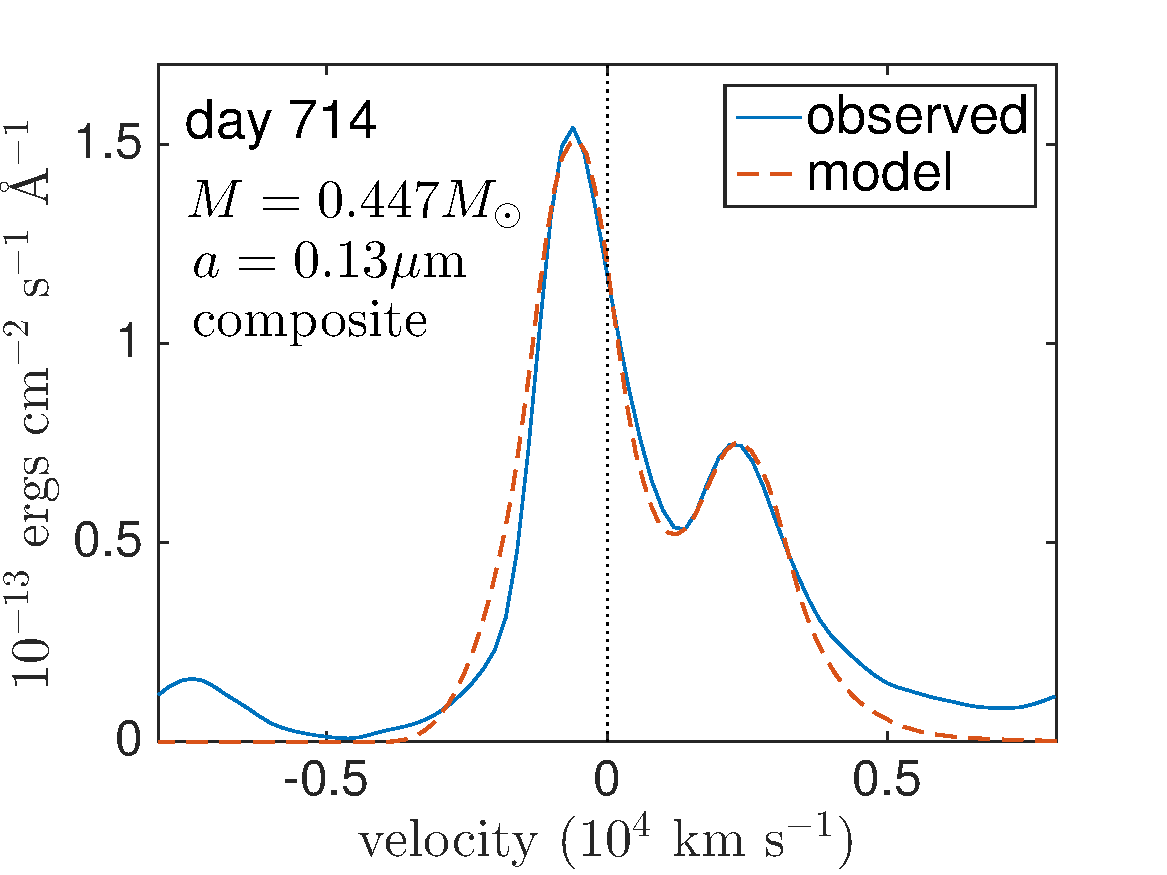
\includegraphics[trim =0 20 0 0,clip=true,scale=0.33]{chapters/chapter5/images/silicates_take2/OI/composit_Dwek.pdf}
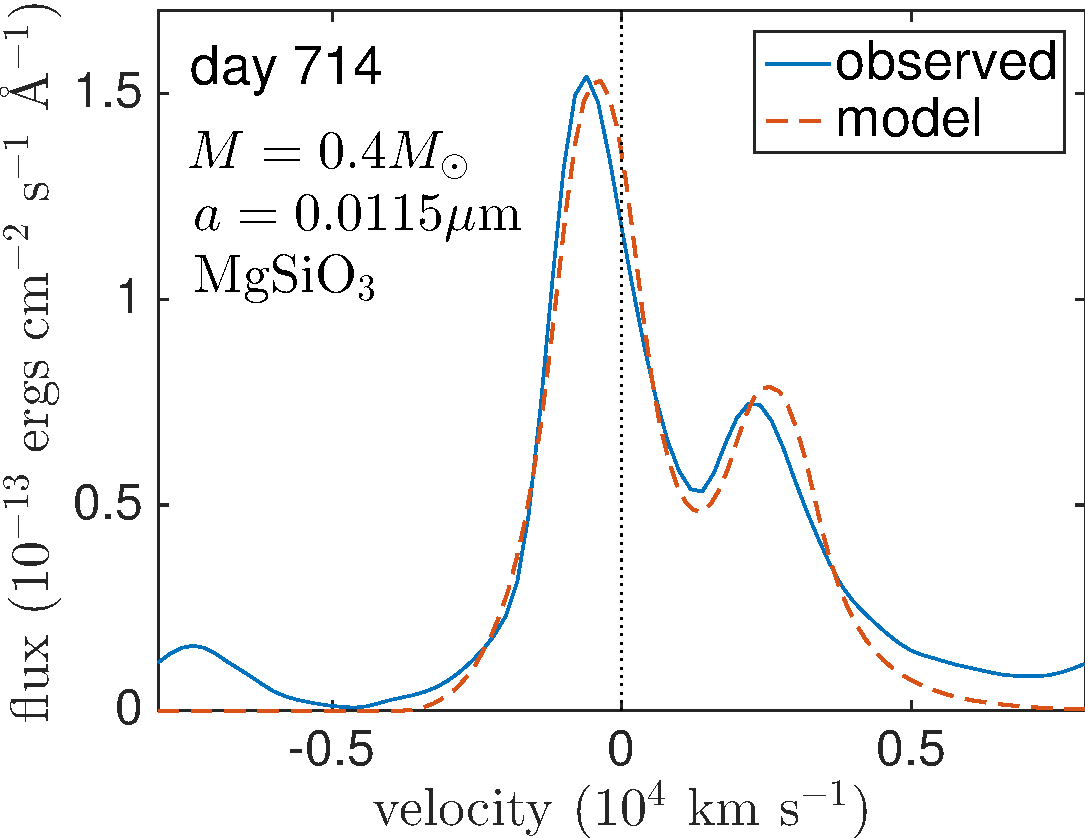
\includegraphics[trim =25 20 0 0,clip=true,scale=0.33]{chapters/chapter5/images/silicates_take2/OI/MgSiO3_Dwek.pdf}
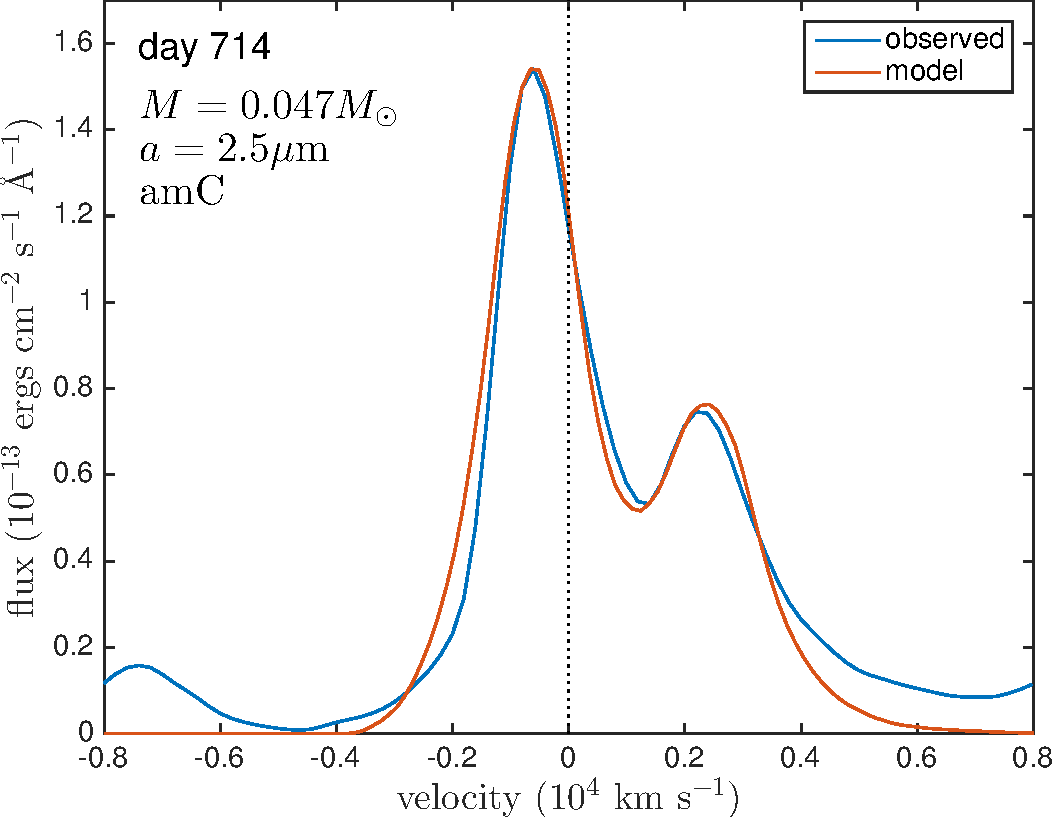
\includegraphics[trim =25 20 0 0,clip=true,scale=0.33]{chapters/chapter5/images/silicates_take2/OI/AmC_Dwek.pdf}
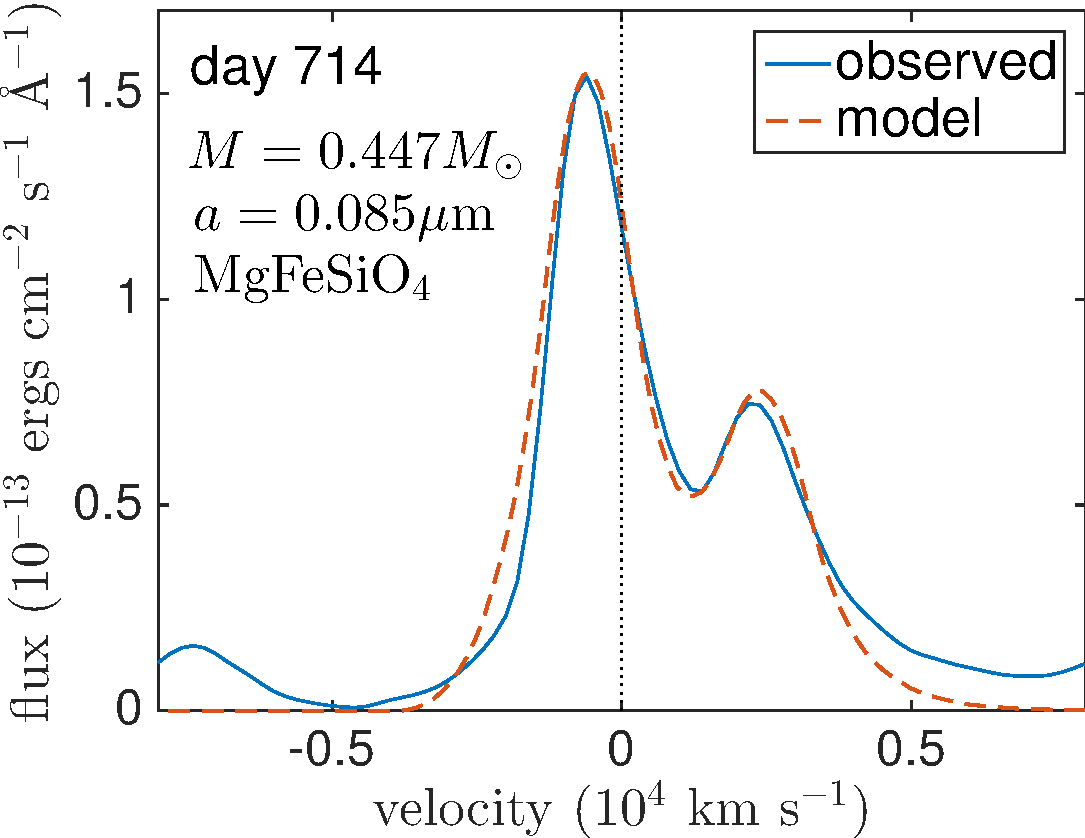
\includegraphics[trim =25 20 0 0,clip=true,scale=0.33]{chapters/chapter5/images/silicates_take2/OI/MgFeSiO4_Dwek.pdf}

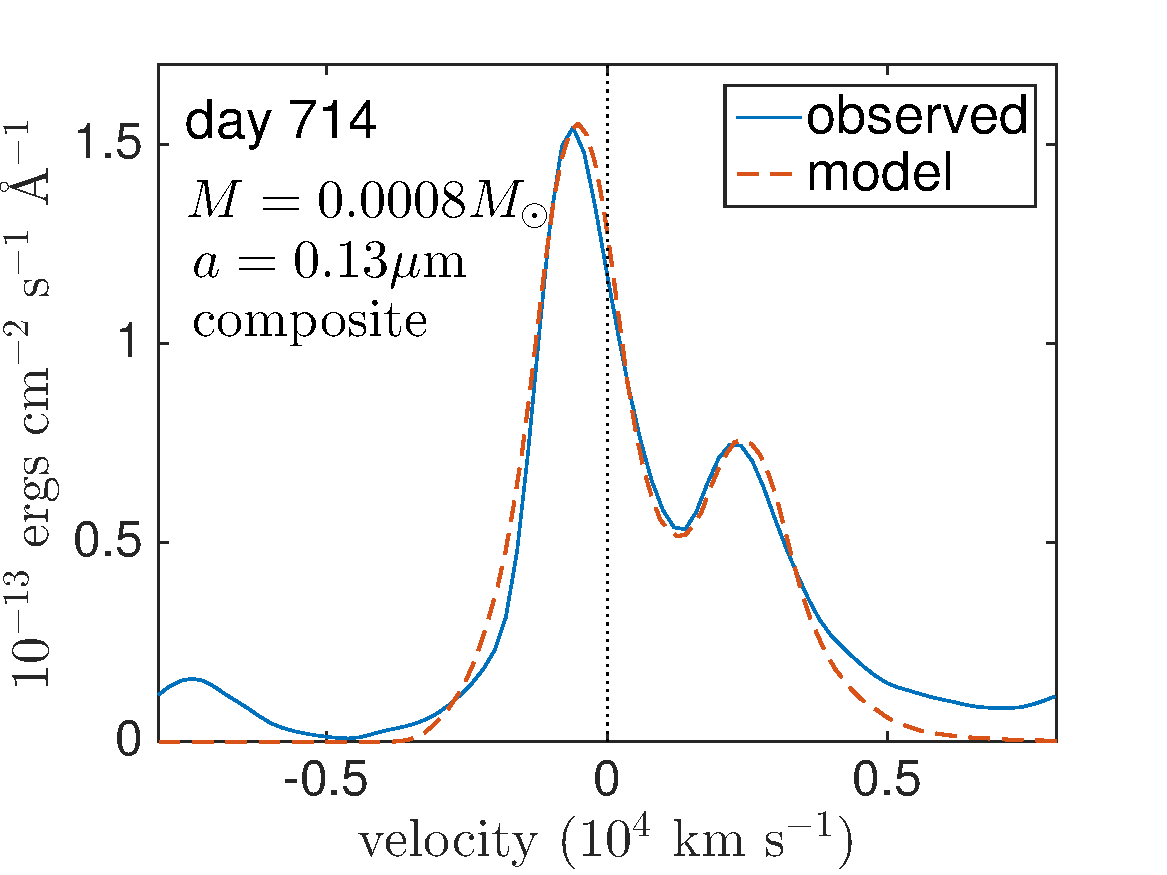
\includegraphics[trim =0 0 0 -25,clip=true,scale=0.33]{chapters/chapter5/images/silicates_take2/OI/composit_bestfit.pdf}
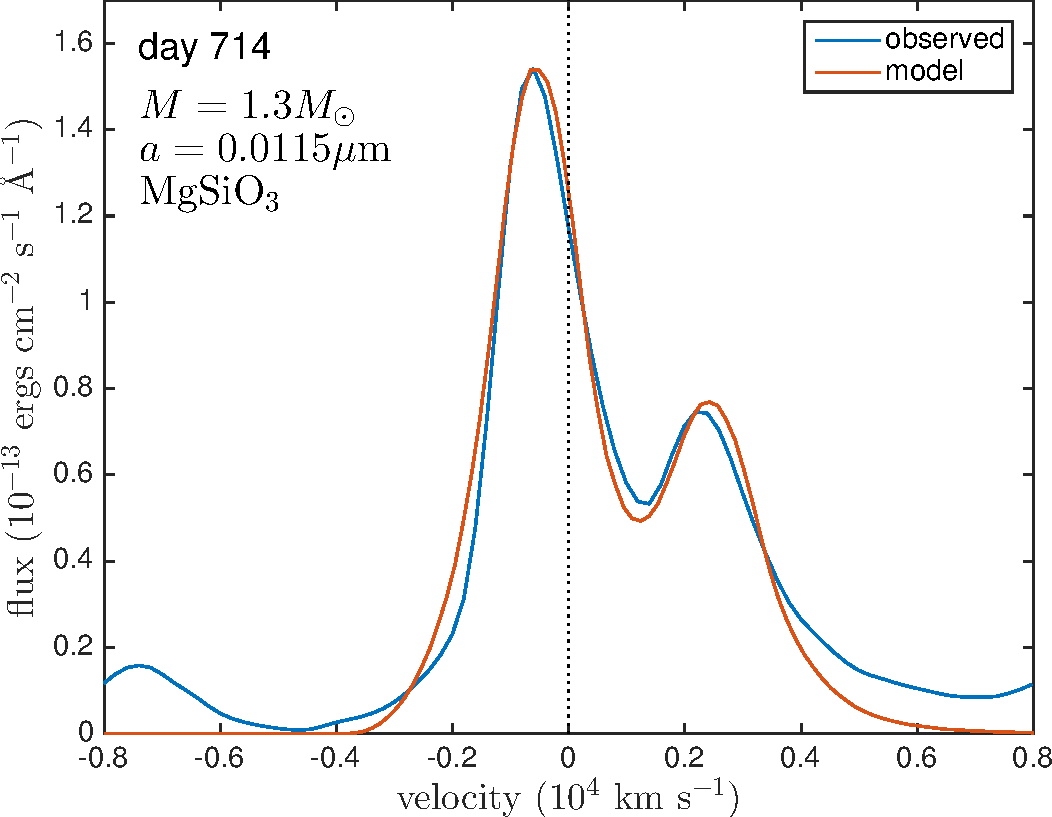
\includegraphics[trim =25 0 0 -25,clip=true,scale=0.33]{chapters/chapter5/images/silicates_take2/OI/MgSiO3_bestfit.pdf}
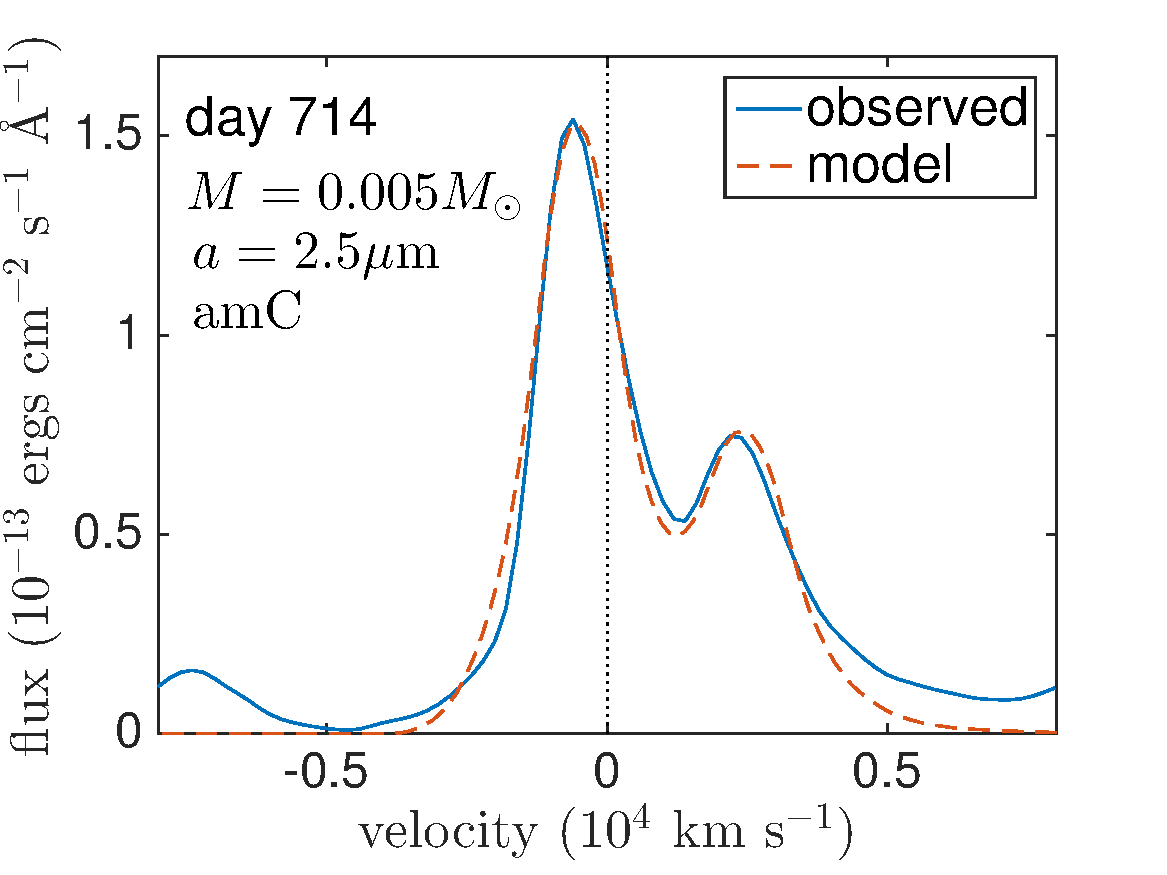
\includegraphics[trim =25 0 0 -25,clip=true,scale=0.33]{chapters/chapter5/images/silicates_take2/OI/AmC_bestfit.pdf}
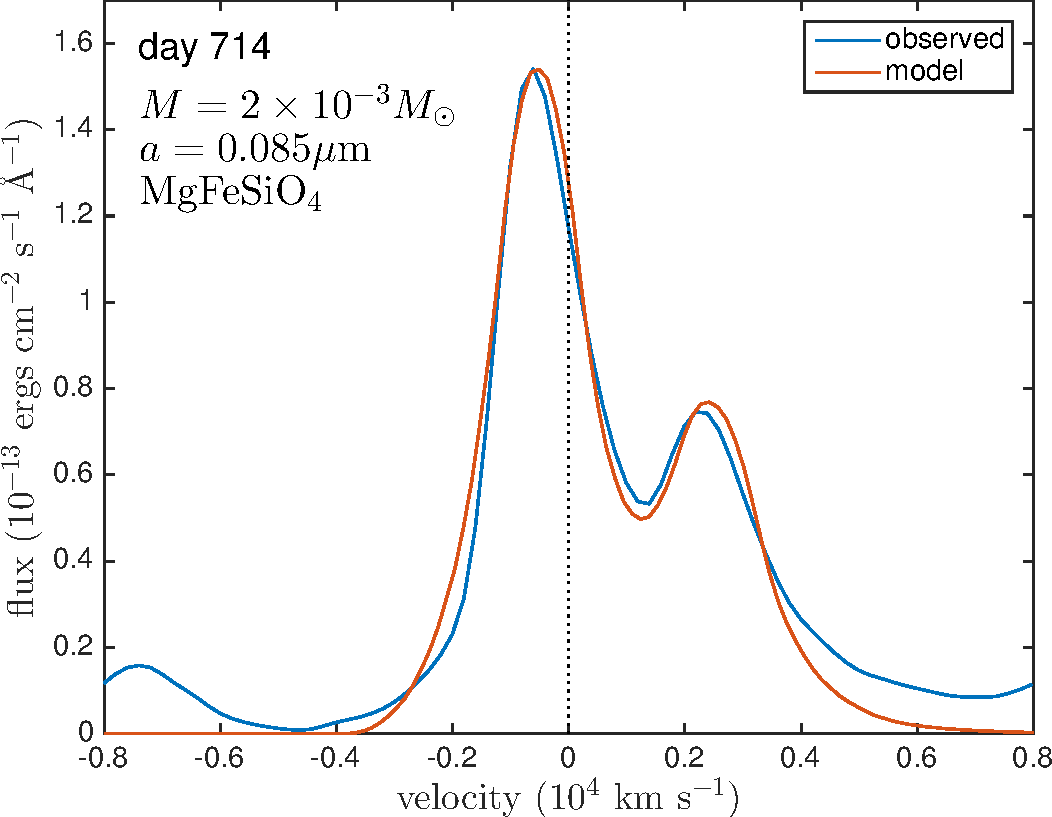
\includegraphics[trim =25 0 0 -25,clip=true,scale=0.33]{chapters/chapter5/images/silicates_take2/OI/MgFeSiO4_bestfit.pdf}

\caption{[O~{\sc i}]$\lambda$6300,6363~\AA\ models using different grain 
species and dust masses.  Models using the dust masses presented by DA15 
are on the top and models using our minimum required dust masses are on 
the bottom.  From left to right the species are composite grains (82\% 
MgSiO$_3$ and 18\% amorphous carbon by volume), pure MgSiO$_3$, pure 
amorphous carbon and pure MgFeSiO$_4$.  A density distribution with 
$\beta=1.3$ was adopted with a filling factor $f=0.09$ and an effective 
clump radius $R_{eff}/R_{out}=0.044$. The ratio between the 
doublet components was 2.2. All other parameters are the same as in 
Table \ref{clumped1}.}
\label{Dwek_models_OI}
\end{figure*}
\end{landscape}
The [O~{\sc i}] models can display similar profiles for substantially 
different dust masses.  This is a result of the relatively high optical 
depths within the clumps themselves. If a clump is optically thick then 
the majority of radiation that hits it will be absorbed and the profile 
becomes insensitive to how much dust is actually contained within the 
clump.  For our [O~{\sc i}] minimum dust mass models, the optical depths 
within a clump over an effective clump radius $R_{eff}$ at 6300\AA\ are 
around $\tau_{clump} \approx 0.4$.  Over the entire nebula optical depths 
are very high and $\sim$72\% of the total flux is absorbed.  Increasing the 
total dust mass therefore has only a small effect on the emergent line 
profile and once $\tau_{clump}>1$ then the line profile remains unchanged 
for increasingly large dust masses.  It is because of this fact that we 
present only the smallest dust mass capable of reproducing the [O~{\sc i}] 
profiles seen in Figure \ref{Dwek_models_OI}.  The insensitivity of the 
[O~{\sc i}] profiles to dust mass is not the case for the H$\alpha$ 
profile models (where $\tau_{clump} < 0.05$ for all of our models) and the 
H$\alpha$-fit dust masses presented in Figure \ref{Dwek_models_Ha} 
therefore represent the most sensitive diagnostic of the dust mass for 
each grain type.  All of our models discussed in previous sections have 
significantly smaller clump optical depths ($\tau_{clump}<0.1$), making 
them sensitive to dust mass variations.

For all the [O~{\sc i}] line profile models, except for those using pure 
MgSiO$_3$ or pure Mg$_2$SiO$_4$ dust, the required dust masses are 
significantly less than those proposed by DA15. The [O~{\sc i}] profile 
obtained using DA15's very large MgSiO$_3$ dust mass of 0.4~M$_{\odot}$ 
provides a reasonable fit, but the same dust mass significantly 
overestimates the blueshifting of the H$\alpha$ line 
(Figure~\ref{Dwek_models_Ha}). We can place an upper limit on the 
mass of pure MgSiO$_3$ on day 714 of 0.07~M$_\odot$, as this 
is the highest mass for which a fit to the observed H$\alpha$ profile can 
be obtained (Figure~\ref{Dwek_models_OI}).

Pure MgSiO$_3$ is extremely glassy, with very high albedos in the optical 
for a wide range of grain radii.  At grain radii small enough to reduce 
the albedo to $\omega \approx 0.6$, in order to fit the observed line 
profiles, the extinction efficiency in the optical becomes extremely low 
(see Figure \ref{albedo_grain}), with large masses of dust therefore 
required in order to produce even a small amount of line absorption. 
However, for a given albedo, the extinction efficiencies increase by large 
factors if either carbon or iron is included in the grain. In the 
composite grain model the amorphous carbon component dominates the overall 
extinction due to its much larger extinction efficiency at small grain 
radii. Similarly, for MgFeSiO$_4$ (or Mg$_{0.5}$Fe$_{0.5}$SiO$_3$) grains
the iron component leads to much larger optical and IR extinction
efficiencies and much lower dust mass upper limits.
If the dust that formed at early epochs contained some fraction of 
elements such as carbon, iron or aluminium, yielding `dirtier' silicate 
grains or composite grains, then fits to the observed blue-shifted line 
profiles imply low dust masses. We conclude that for dust masses as large
as 0.07~M$_\odot$ to have been present in SN~1987A's ejecta as early as 
days 600-1000 then the dust would have to have been formed of glassy pure 
magnesium silicates.


%%%%%%%ADDITIONAL CONTENT%%%%%%%%%%%%%%%%%
\subsection{Unattenuated line fluxes}

The evolution of the SN~1987A H$\alpha$ and [O~{\sc 
i}]$\lambda$6300,6363~\AA\ line fluxes over time has been discussed 
previously by, for example, \citet{Li1992}, \citet{Xu1992} and 
\citet{Kozma1998b}. We may use our clumped models to predict the 
unattenuated 
emitted line fluxes and consider their evolution through time.  For each 
model, the fraction of the total line energy absorbed by the dust was 
predicted.  We determined the total flux for each observed line profile 
and used the absorbed fraction from our clumped models for $a=3.5\mu$m to 
predict the undepleted flux of the line before attenuation by the dust.  
Gaps in the observed data due to contamination by narrow line emission 
were interpolated over in order to estimate the flux of the broad line 
component. The observed H$\alpha$ luminosities and predicted undepleted 
luminosities are given in Table \ref{tau_e} along with the energy fraction 
absorbed by the dust in each model. No correction has been made for 
interstellar extinction along the sightline to SN~1987A.
There is very little change in 
these values if we adopt the models with $a=0.6~\mu$m instead of 
$a=3.5~\mu$m.  Plots of the observed and undepleted line luminosities are 
given for all modelled epochs of H$\alpha$ and [O~{\sc i}] in Figure 
\ref{undep}.

We also present power-law fits to the time evolution of the unattenuated 
H$\alpha$ and [O~{\sc i}] line fluxes.  For H$\alpha$, we find that 
$L_{H\alpha}(t) \propto t^{-4.15}$ between days 714 and 3604.  We can 
compare this value to the theoretical time dependence of the flux of a 
recombination line based on the dynamics of the ejecta.  For an 
environment in a Hubble-type flow $r=vt$.  For a frozen-in ionization 
structure, the mean intensity of a recombination or collisionally-excited 
line per unit volume is locally proportional to the product of the 
densities of the recombining species i.e. $J_{H\alpha} \propto n_e n_p 
\propto n_e^2$.  The total luminosity of the line is therefore dependent 
on the volume $V$ as $L_{H\alpha} \propto 1/V $.  Assuming a constant 
maximum expansion velocity, the luminosity should vary with time as 
$L_{H\alpha}(t) \propto t^{-3}$.

This relationship is only true for an constant ionization fraction.  This 
``freeze-out" phase is estimated to have begun at $\sim 800$ days and 
first sets in at lower density high velocity regions, gradually moving 
inwards with time \citep{Danziger1991,Fransson1993}.  Since our modelling 
begins at day 714, the ionization fraction in the inner higher density 
regions is likely still decreasing due to recombination during our first 
two epochs.  This presumably accounts for the slightly steeper 
$L_{H\alpha}(t) \propto t^{-4.15}$ that we find across all epochs.  
\citet{Kozma1998b} estimate that H$\alpha$ emission from the outer regions 
begins to dominate over H$\alpha$ emission from core regions for t $>$ 
900 days. If earlier epochs are ignored, the last five epochs ($t \ge 
1862$ days) plotted in (Figure \ref{undep}) exhibit a shallower trend that 
is in good agreement with the expected $L_{H\alpha}(t) \propto t^{-3}$ 
evolution.

The [O~{\sc i}]$\lambda$6300,6363~\AA\ doublet exhibits a much 
steeper evolution, $L_{[OI]}(t) \propto t^{-7.2}$, than the H$\alpha$ line 
(Figure \ref{undep}). These collisionally excited lines are very sensitive 
to the gas temperature, with emissivities that fall to low values for 
temperatures below $\sim$3000~K. The models of \citet{Li1992,Kozma1998a} 
predict that the gas temperature in the relevant [O~{\sc i}] emitting 
regions should have fallen below 1000~K after day $\sim$1000.


\begin{figure}
\centering
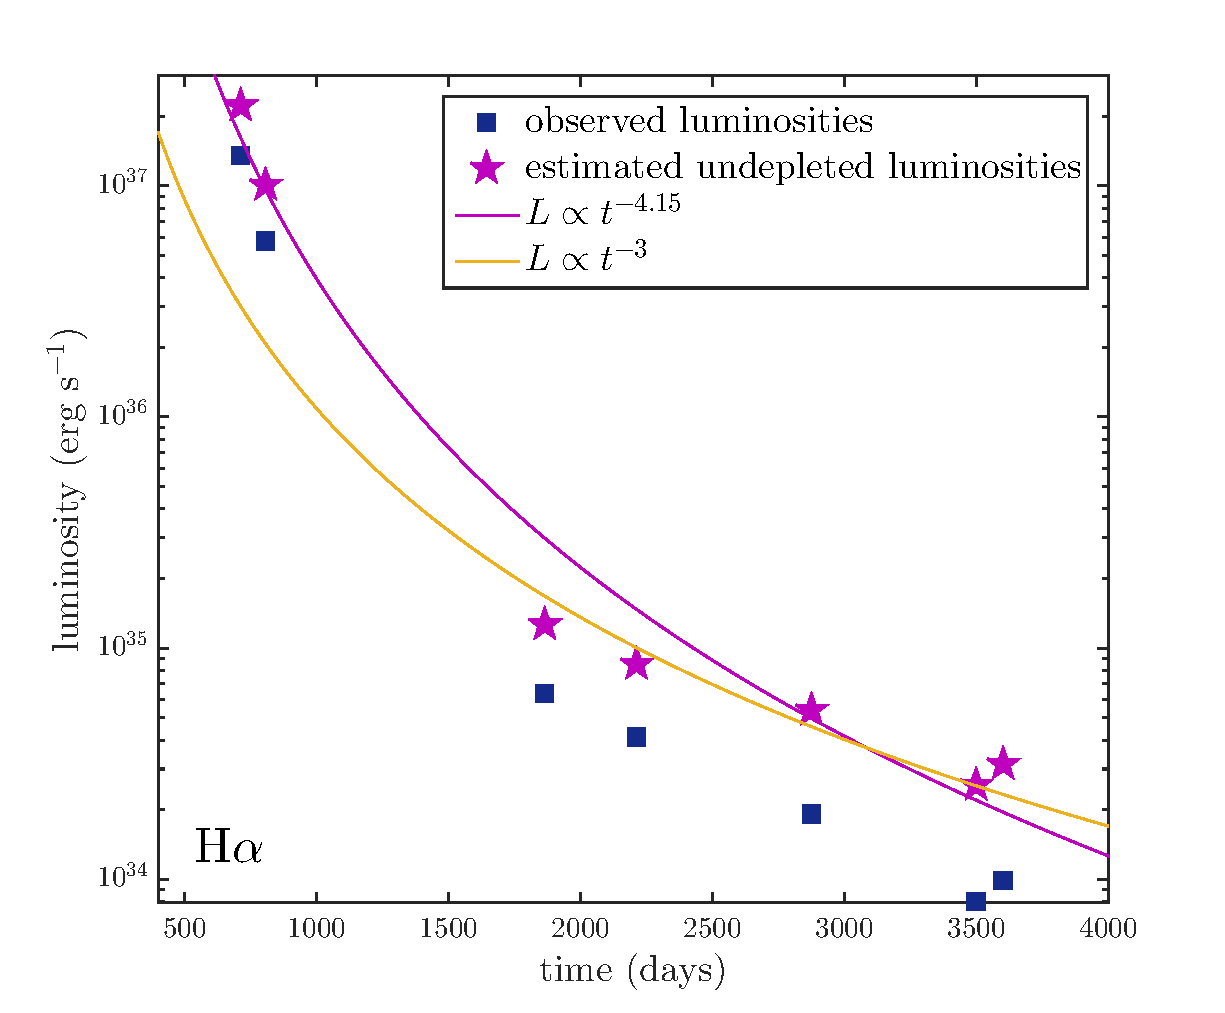
\includegraphics[clip=true,scale=0.6]{chapters/chapter5/images/undep_fluxes_Ha.pdf}

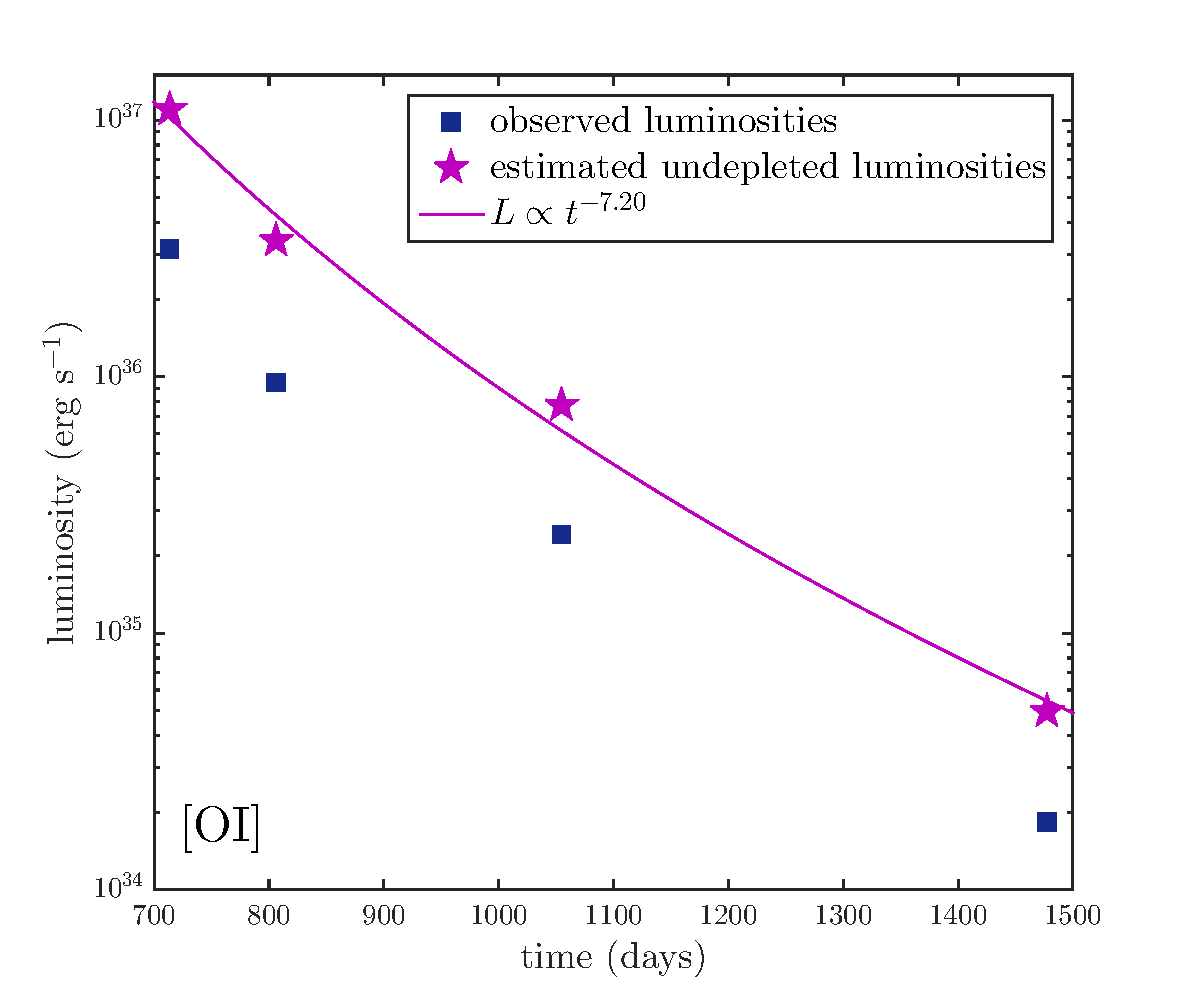
\includegraphics[clip=true,scale=0.6]{chapters/chapter5/images/undep_lum_OI.pdf}
\caption{Predicted undepleted luminosities for the H$\alpha$ line 
\textit{(above)} and [O~{\sc i}]$\lambda$6300,6363~\AA\ doublet 
\textit{(below)} presented with the best power-law fit to the data.}
\label{undep}
\end{figure}



\section{Discussion}
\label{discuss}

Using Monte Carlo models that consider both the absorbing and scattering 
effects of dust, we have modelled the evolution of the H$\alpha$ and 
[O~{\sc i}]~$\lambda$6300,6363~\AA\ line profiles over time, enabling us 
to place constraints on the evolution of newly formed dust in the ejecta 
of SN 1987A.

As can be seen in Figure \ref{d1862_3604}, even a small degree of 
asymmetry in observed supernova line profiles can be indicative of dust 
formation within the ejecta.  In addition to this, a line profile that is 
consistently asymmetric through time requires increasingly large dust 
masses to account for a similar degree of blue-shifting since the 
expansion of the ejecta would otherwise cause the dust optical depth to 
the edge of the ejecta to be reduced.

In Section \ref{dwek} we compared our results with those of \citet{Dwek2015} and 
concluded that large dust masses can only have been present at early 
epochs if the grains were formed purely of glassy magnesium silicates that 
contained no iron or carbon component and that even for pure magnesium 
silicates no more than 0.07~M$_\odot$ can have been present. We now 
compare our results with those of \citet{Lucy1989} and W15.

\citet{Lucy1989} analysed the [O~{\sc i}]~$\lambda$6300,6363~\AA\ doublet 
for SN~1987A and estimated dust optical depths for a number of epochs. 
They translated these into dust masses for day 775 only. From our smooth 
flow modelling of the [O~{\sc i}] doublets we obtain $\tau_V \approx 3.60$ at day 
714 and $\tau_V \approx 2.86$ at day 806.  These values are higher 
than the values given by \citet{Lucy1989} who derived $\tau_V=1.19$ at day 
725 and $\tau_V=1.25$ at day 775.  The value of the assumed albedo 
accounts for the majority of this discrepancy.  \citet{Lucy1989} 
considered line profiles before and after dust condensation and concluded 
that any evidence of an extended red scattering wing was unconvincing.  
Accordingly, they adopted a model with perfectly absorbing dust ($\omega = 
0$).  For our amorphous carbon models for the [O~{\sc 
i}]~$\lambda$6300,6363~\AA\ profile using a grain radius $a=0.35\mu$m, we 
obtain an albedo of approximately $\omega = 0.5$ at $\lambda=6300$ \AA.

\begin{landscape}
\begin{figure*}
\begin{center}
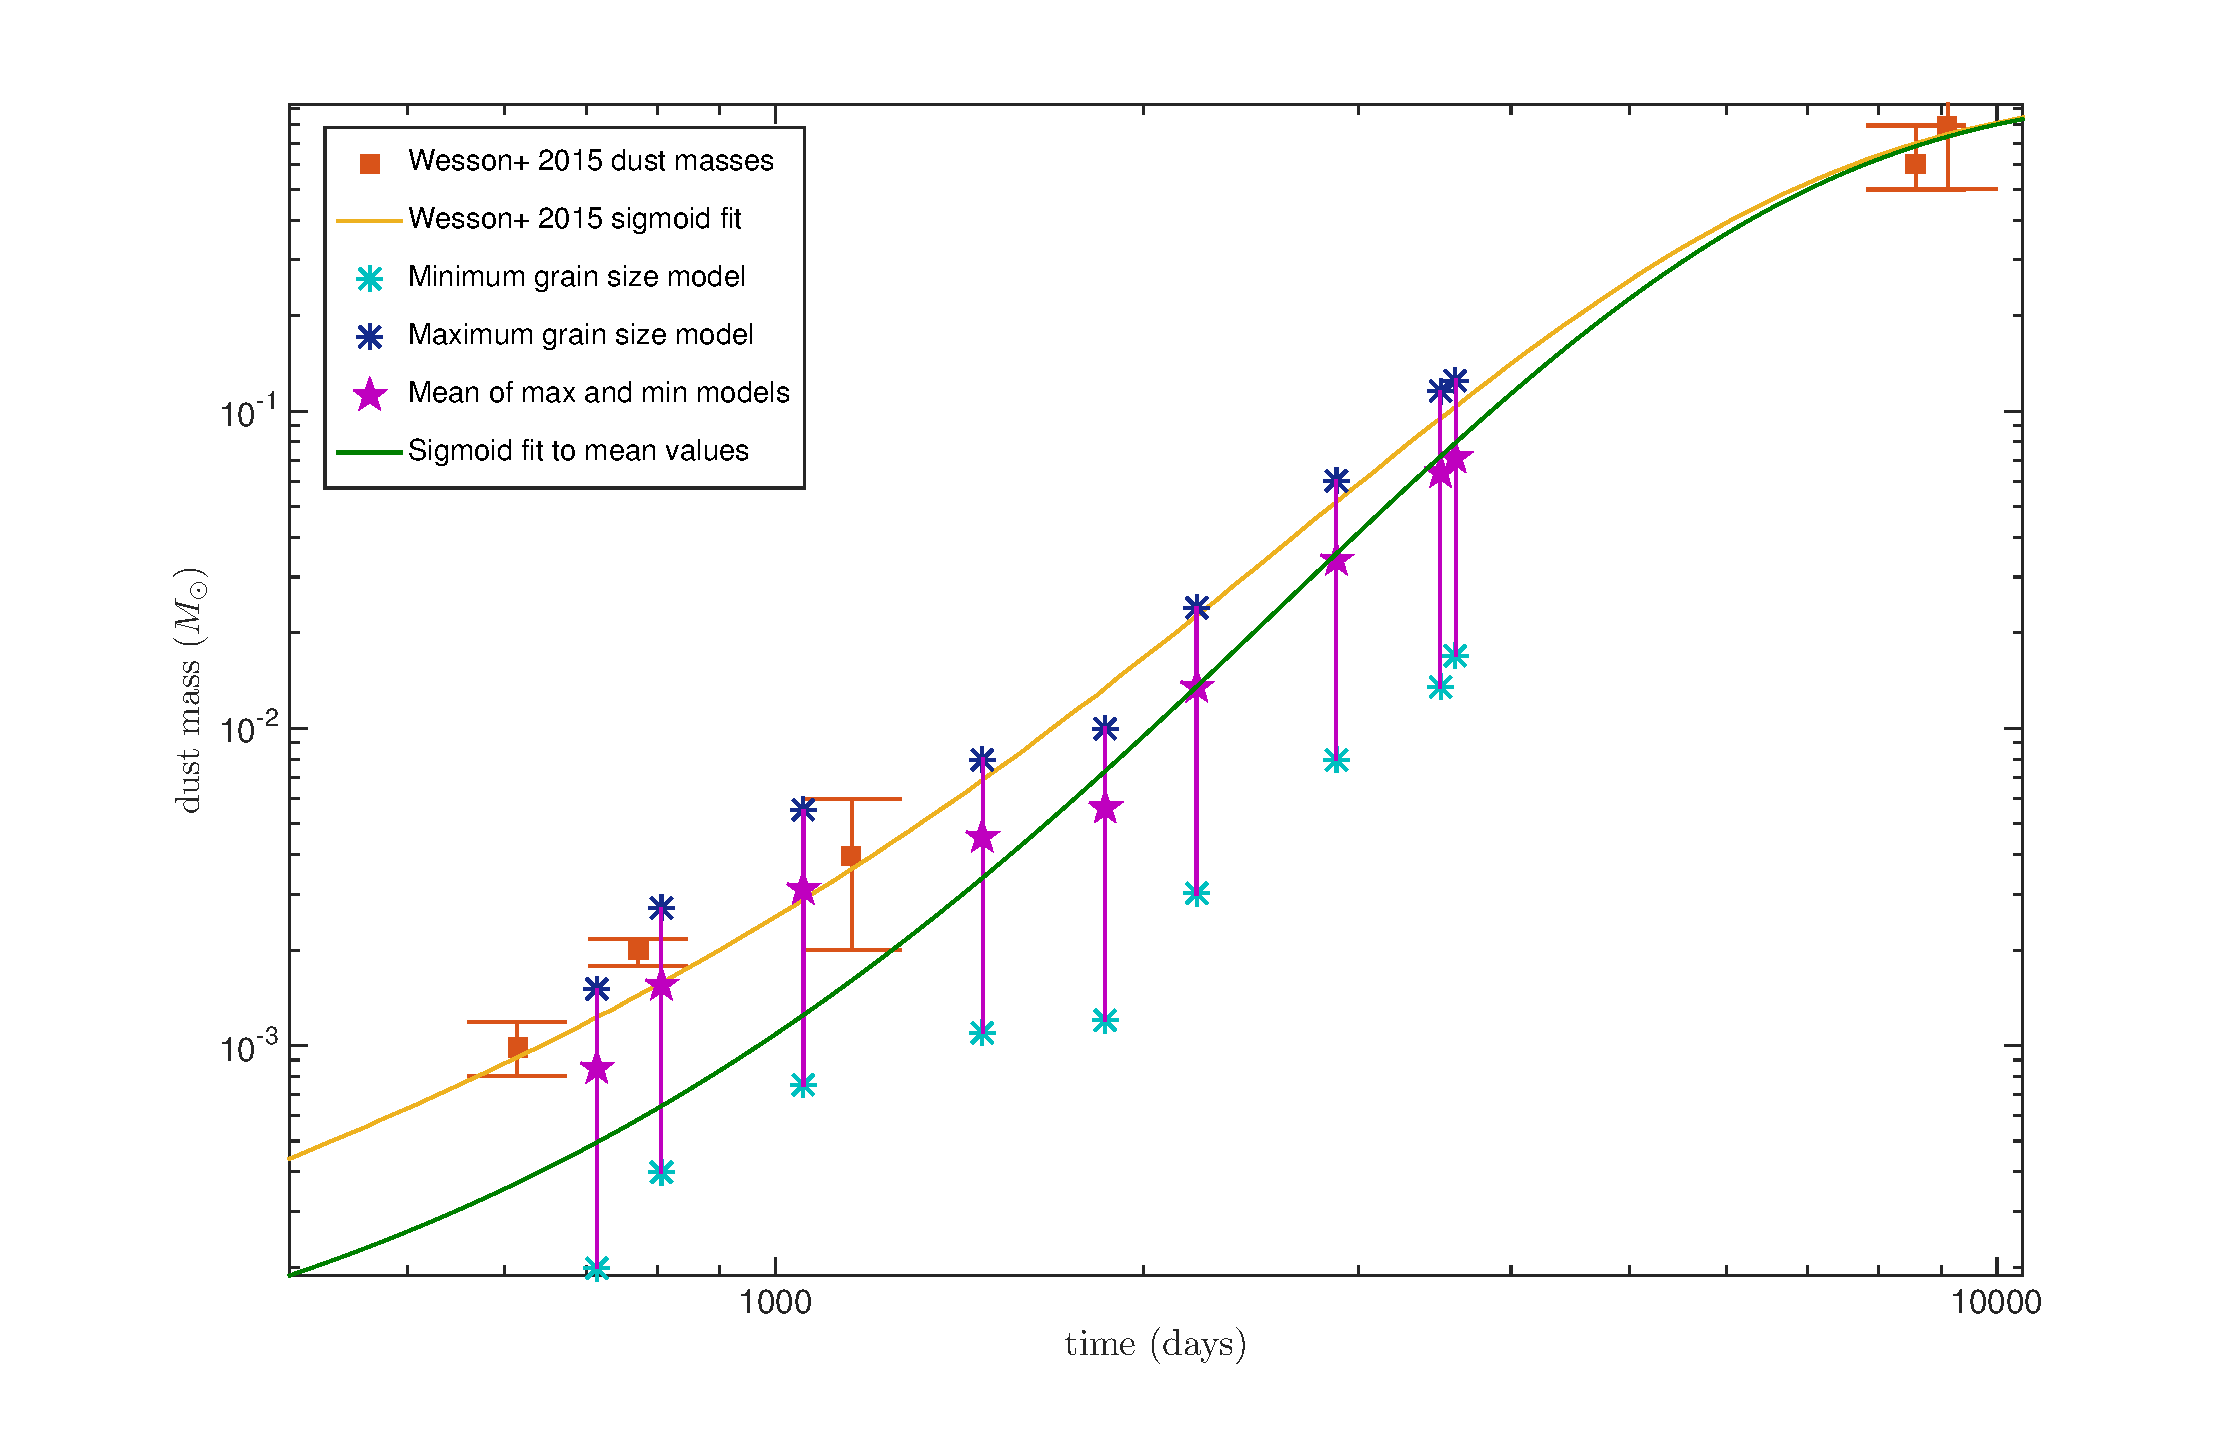
\includegraphics[trim =70 30 85 15,clip=true,scale=0.52]{chapters/chapter5/images/Mdust_evol7.pdf}
\caption{Derived dust masses for SN~1987A as a function of epoch. 
\textit{Red squares -} dust masses derived by W15 
from their photometric SED modelling of SN 1987A. \textit{Yellow line} - 
W15's sigmoid fit to 
their values. \textit{Dark and light blue asterisks -} maximum 
($a=3.5~\mu$m) and 
minimum ($a=0.6~\mu$m) dust masses respectively for the [O~{\sc i}] models 
for $t \le 1478$ days and for the H$\alpha$ models for $t \ge 1862$ days. 
\textit{Purple 
stars -} predicted dust masses calculated as the mean of the maximum and 
minimum dust masses.
\textit{Green line -} sigmoid fit 
to our predicted dust masses.}
\label{Mdust}
\end{center}
\end{figure*}
\end{landscape}

The dust masses derived by \citet{Lucy1989} at day 775 (e.g. $M_{dust}=4.4 
\times 10^{-6} M_{\odot}$ for amorphous carbon) are  
different to those obtained from our smooth dust modelling of the [O~{\sc 
i}]~$\lambda$6300,6363~\AA\ doublet at day 806 ($M_{dust}=1.5 \times 
10^{-4} M_{\odot}$ for amorphous carbon).  There are three main reasons 
for the discrepancy.  Firstly, the albedo is significantly larger in our 
modelling as already discussed.  A larger dust mass is therefore required 
to produce the same amount of absorption.  Secondly, to match the extended 
red wing our required grain radius is considerably larger than the small 
grains ($a < 0.1\mu$m) adopted by \citet{Lucy1989}. Larger grain radii 
reduce the total cross-section of interaction and so a greater dust mass 
must be present to compensate for this. Finally, the adopted maximum 
velocity (4000~km~s$^{-1}$) in our model is larger than the value adopted 
by \citet{Lucy1989} (1870~km~s$^{-1}$).  The larger value of $V_{max}$ 
increases the total volume of the ejecta significantly and therefore 
significantly more dust is required to produce the same optical depth.

\citet{Lucy1989} also noted that the dust optical depth increased rapidly 
after day 580 and that the rate of increase of the dust optical depth 
appeared to slow between day 670 and day 775, the latest day that they 
considered.  Our results, for both clumped and smooth models, suggest that 
the dust optical depth actually drops between day 714 and day 806 before 
starting to increase again at later epochs.  This is consistent with the 
results of \citet{Lucy1989} where the slowing rate of increase of dust 
optical depth could be consistent with a turning point subsequent to day 
775.

We can also compare our dust masses with the mass estimates derived from 
SED-fitting by W15 (see Figure \ref{Mdust}).  W15 used a sigmoid fit to 
their dust mass evolution, of the form

\begin{equation}
M_d(t)=ae^{be^{ct}}
\end{equation}
 
\noindent where $a=1.0M_{\odot}$ (representing the limiting dust mass), 
$b=-8.53$ and $c=-0.0004$.  Both their dust masses and this sigmoid fit 
are shown in Figure \ref{Mdust}.  It exhibits an initial period of slow 
growth in mass followed by an intermediate period of accelerating growth 
followed by another slowing until a plateau is ultimately reached.  In 
this sense it may be representative of the process of dust 
formation whereby initial conditions appropriate for grain growth 
gradually develop until optimal conditions are reached at an intermediate 
epoch when grain growth is at its fastest before conditions once again 
deteriorate and the rate slows again (as discussed by W15).  Performing a 
least-squares regression to this function using just our own derived 
clumped dust masses, we obtain a sigmoid fit with coefficients 
$a=1.0M_{\odot}$, $b=-10.0$ and $c=-0.0004$.  These values are 
remarkably similar to those derived by W15.  This sigmoid fit is also 
plotted in Figure \ref{Mdust}.

We find that at all epochs the dust masses derived by W15 are entirely 
within the dust mass ranges determined by our models.

Our sigmoid fit to the mean of the maximum and 
minimum dust masses does not take into account any systematic effects of 
grain growth.  At earlier epochs, whilst grains are 
still small relative to later epochs, the lower bound to the dust mass 
estimates may be more representative than the upper end; the reverse would 
be true at later epochs.
%%%%%%%new%%%%%%%%%%
This is in contrast to the sigmoid fit of W15, whose fits to their early 
epoch SEDs used an MRN distribution with grain radii between 0.005~$\mu$m 
and 0.25~$\mu$m, whilst their fits to their last two epochs required grain 
radii between 3.005~$\mu$m and 3.25~$\mu$m. The dust masses used for their 
sigmoid fit thus accounted the effects of grain growth between the earlier 
and later epochs. As mentioned, we could not fit the extended red wings of 
the profiles at early epochs using an MRN distribution.  W15 found that at 
their earlier epochs they could not obtain SED fits with grain radii as 
large as $\sim 1.0~\mu$m. However, they did not consider radii in between 
these size ranges, such as the grains with $a \approx 0.6~\mu$m that we 
require at earlier epochs.  For SED modelling it is generally the case that 
the larger the grain size used, the less dust is required to produce the 
same level of flux.  This may account for the differences between W15's 
earlier epoch dust masses and our own minimum dust mass estimates at 
similar epochs.  The models of W15 used 15\% silicate dust, in contrast to 
our models which used 100\% amorphous carbon dust.  This could also 
contribute to the differences at early epochs, as could the use of 
different sets of optical constants - we used the BE amorphous carbon 
optical constants of \citet{Zubko1996} whereas W15 used AC constants from 
\citet{Hanner1988}.  W15 found that in order to fit early epoch SEDs epochs 
(e.g. day 615) with Zubko ACH2 constants, smaller inner and outer ejecta 
radii were needed, with half as much dust ($5.0 \times 10^{-4}M_{\odot}$) 
compared to the Hanner AC results.

W15 derived a maximum possible grain size at late epochs, concluding that 
the grains could not be larger than $\sim 5~\mu$m by day 8515. This is 
consistent with the maximum grain radii that we derive at our latest 
epochs.  We find that grain radii most likely cannot have exceeded $\sim 
3.5~\mu$m at day 3604 - the dust mass that we obtain using this grain 
radius is similar to the value predicted by W15's sigmoid fit at that 
epoch.

The relationship between ejecta dust grain radii and post-explosion 
time is important for understanding the likelihood of dust surviving the 
passage of a reverse shock propagating back through the ejecta. By the 
time the effects of a reverse shock begin to appear in the line profiles 
(around day 5000), our models imply that the grains could already be as 
large as several microns in radius and are likely to be larger than $\sim 
0.6~\mu$m. Grains as large as this are more likely to survive destruction 
by sputtering in supernova reverse shocks and in interstellar shocks 
\citep{Silvia2010, Silvia2012, Slavin2015}.
It has been suggested that very large grains (radii up to 4.2$~\mu$m) 
formed in the ejecta of SN 2010jl within a few hundred days after the 
explosion \cite{Gall2014}. The grain radii that W15 and ourselves obtain 
for SN~1987A at very late epochs are nearly as large as found by 
\citet{Gall2014} for SN~2010jl, with both results suggesting that grains 
large enough to survive the destructive force of a reverse shock have 
formed by a few hundred days post-explosion. 

The dust masses obtained from our modelling of SN~1987A's line profiles 
support the conclusion of W15 that even after $\sim$3000 days the dust 
mass was still only a fraction of its current value. This contrasts with 
the results of \citet{Sarangi2015} whose grain chemistry models predict 
that ejecta dust masses should plateau by around 5 years after the 
explosion. Our results show that SN~1987A's dust mass had reached 
the order of $0.1M_{\odot}$ by day 3604.  Since its present dust mass is 
several times larger than this (\citet{Matsuura2015}, W15), a 
substantial fraction of the current dust mass must have condensed after 
this epoch, in agreement with the conclusions of W15.

Ideally, our models would cover the entire evolution of SN 1987A's 
H$\alpha$ line profiles up to the present day.  However, the excitation of 
gas in the outer edges of the ejecta by the reverse shock after $\sim$ day 
5000 results in significant broad and asymmetric emission that 
dominates the original line profile \citep{Fransson2013}.  In addition to 
this, the narrow lines from the equatorial ring start to become so 
strong relative to the declining broad H$\alpha$ profile that, 
post-removal, not enough of the broad profile remained to be 
able to reliably infer information from the profile structure. These 
factors may be 
common to some other CCSNe that have interactions with surrounding 
circumstellar material. Care should also be taken to ensure that any 
observed late-time line profiles being modelled are not in fact the 
product of a light echo reflecting the spectrum from near maximum light. 
Nonetheless, detailed line modelling of asymmetric line profiles has 
proved effective in determining dust masses in the ejecta of SN~1987A at 
multiple epochs during the first ten years after outburst. The method 
clearly has wider application to other supernovae.


\section{Conclusions}

We have investigated the effects of scattering and absorption by ejecta 
dust on supernova line profile shapes and the different characteristic 
features that may be produced.  In particular, attention is drawn to the 
fact that a classical blue-shifted peak and asymmetric profile with most 
flux on the blue side is not the only profile type that can signify the 
presence of dust. In the case of strong dust scattering, line profiles can 
have the majority of their flux on the red side. Even with just some dust 
scattering, profiles can often exhibit an extended red scattering wing, 
although care should be taken to ascertain that this cannot be accounted 
for by electron scattering (electron scattering optical depths should 
usually only be significant at very early epochs, $<$ 200 days). The line 
peak should always lie on the blue side, with a line peak velocity that 
will often correspond to the minimum velocity at the inner edge of the 
ejecta shell. If not obscured by narrow circumstellar [N~{\sc ii}] 
6584~\AA\ emission, a pronounced shoulder or corner may be present on the 
red side of the profile, also corresponding to the minimum velocity at the 
inner edge of the ejecta shell.

We have modelled the H$\alpha$ and [O~{\sc i}]~$\lambda$6300,6363~\AA\ 
line profiles from SN~1987A over a range of epochs and have obtained dust 
masses of the order of $0.1M_{\odot}$ by day 3604.  We derive a sigmoid 
fit to our dust mass data that predicts a current dust mass of 
0.68$M_{\odot}$, in line with current SED-based dust mass estimates for 
SN~1987A.  We find that large grains are necessary in order to reproduce 
the both the extended red scattering wings and the asymmetry seen in 
several of the lines and that grains larger than $0.6~\mu$m have formed by 
day 714, while by day 3604 grain radii of $\sim 3.5~\mu$m are needed. We 
find from fits to the H$\alpha$ profile that dust masses cannot have 
exceeded a few$\times10^{-3}$~M$_\odot$ on day 714 for all the grain types 
investigated, apart from glassy pure magnesium silicate grains, for which 
up to 0.07~M$_\odot$ can be fitted.

The observed red-blue line asymmetries persist right through to day 3604 
and beyond - if no further dust had formed after day $\sim$800 then the 
expansion of the ejecta shell dust shell would cause dust optical depths 
to drop rapidly with time thereafter, leading to the disappearance of 
red-blue asymmetries. Just to maintain the observed degree of red-blue 
asymmetry seen at the earlier epochs therefore requires that dust must 
have continued to form beyond those epochs.
